%% GABARIT POUR THÈSE PAR ARTICLES
%%
%% Consulter la documentation de la classe ulthese pour une
%% description détaillée de la classe, de ce gabarit et des options
%% disponibles.
%%
%% [Ne pas hésiter à supprimer les commentaires après les avoir lus.]
%%
%% Déclaration de la classe avec le type de grade
%%   [l'un de LLD, DMus, DPsy, DThP, PhD]
%% et les langues les plus courantes. Le français sera la langue par
%% défaut du document. L'option 'bibsection' permet de créer des
%% bibliographies par chapitre présentées sous forme de section
%% numérotée.
  
% \documentclass[PhD,english,french]{ulthese}
\documentclass[PhD,english,french,nonatbib]{ulthese} % nonatbib car pas compatible avec author-year citation
% \documentclass[PhD,bibsection,english,french,nonatbib]{ulthese}

  %% Encodage utilisé pour les caractères accentués dans les fichiers
  %% source du document. Les gabarits sont encodés en UTF-8. Inutile
  %% avec XeLaTeX, qui gère Unicode nativement.
  \ifxetex\else \usepackage[utf8]{inputenc} \fi

  %% Charger ici les autres paquetages nécessaires pour le document.
  %% Quelques exemples; décommenter au besoin.
  %\usepackage{amsmath}       % recommandé pour les mathématiques
  %\usepackage{ncccomma}      % gestion de la virgule dans les nombres
  %% 
  %%\usepackage[toc]{glossaries}      % gestion du glossaire
  %%\makeglossaries

  %% Utilisation d'une autre police de caractères pour le document.
  %% - Sous LaTeX
  %\usepackage{mathpazo}      % texte et mathématiques en Palatino
  %\usepackage{mathptmx}      % texte et mathématiques en Times
  \usepackage[scaled]{helvet}
  \renewcommand\familydefault{\sfdefault} 
  %% - Sous XeLaTeX
  %\setmainfont{TeX Gyre Pagella}      % texte en Pagella (Palatino)
  %\setmathfont{TeX Gyre Pagella Math} % mathématiques en Pagella (Palatino)
  %\setmainfont{TeX Gyre Termes}       % texte en Termes (Times)
  %\setmathfont{TeX Gyre Termes Math}  % mathématiques en Termes (Times)

  %% Packages ajoutés par moi
  \usepackage{todonotes}            % Notes de TODO avec \todo
  \usepackage{multirow}             % Tables avec lignes fusionnées
  
  \usepackage{alphabeta}            % Lettres grecques hors mode maths
  \usepackage[acronym]{glossaries}  % Glossaire
  \makeglossaries
  \usepackage{appendix}             % Test : Annexes formatées comme voulu
  \usepackage{textgreek}            % Lettres grecques hors formules de maths
  \usepackage{graphicx}             % Affichage d'image
  \usepackage{lscape}               % Rotation en paysage d'un environnement de feuille
  \usepackage[export]{adjustbox}    % Adaptation d'image à une div
%   \usepackage{adjustbox}    % Adaptation d'image à une div
%   \usepackage{listings}
%   \usepackage{xcolor}
  \usepackage{rotating}             % Tourne les figures
  \usepackage{longtable}            % Table sur plusieurs pages
  \usepackage{svg}
  \usepackage{booktabs}             % Tables plus propres avec pre-formatage
  \usepackage{colortbl}             % Couleur dans des tables
  \usepackage{enumitem}             % Circled numbers
  \usepackage{float}                % Positionnement des figures tables plus "facilement" ?
  \usepackage{silence}              % Permet de virer les warnings indésirables
  \WarningFilter{latex}{Label}      % Warnings sur ref multiples mais c'est voulu
  \WarningFilter{glossaries}{Overriding \printglossary}  % Warnings sur le glossaire
  \WarningFilter{glossaries}{overriding `theglossary'}
  
  \usepackage[font=footnotesize]{caption} % Change la taille des textes de caption
%   \usepackage[font=scriptsize]{caption} % Change la taille des textes de caption
  
  \usepackage{titlesec}             % Permet d'utiliser /chapter sans * pour avoir la bonne numérotation
   \titleformat{\chapter}[display]
    {\normalfont\bfseries}{}{0pt}{\Huge}
    
  \usepackage[resetlabels]{multibib}             % Permet de faire des bibliographie par chapitre
  \newcites{A,B}{References,Références}          % Défini une biblio A et B pour le chapitre 1 et 2
  \renewcommand{\bibsection}{\section{\bibname}} % Passe les biblio en tant que section
    
  %% /!\ S'assurer que hyperref est le dernier paquetage chargé.
  \usepackage{hyperref}             % Gestion des hyperliens dans le document
  \hypersetup{colorlinks,allcolors=ULlinkcolor}
  \urlstyle{same}



  
   %%% Personal helper functions
   
   %% Own command to make notes with ref inside text and not into footnote
   % USE :
   %   This is a test to which a note is added\note{test1}{mycounter}
   %   \ref{note:mycounter:test1} Explanation linked to the note
  \newcommand\note[2]{\getid{#1}\label{note:#1:#2}\textsuperscript{\ref{note:#1:#2}}}
  \makeatletter
  \newcommand{\getid}[1]{%
      \@ifundefined{c@#1}
      {% the counter doesn't exist
        \newcounter{#1}\setcounter{#1}{1}%
      }
      {% the counter exists
        \stepcounter{#1}%
      }%
      \def\@currentlabel{\arabic{#1}}
  }
  \makeatother

  
  
  

  %% Options de mise en forme du mode français de babel. Consulter la
  %% documentation du paquetage babel pour les options disponibles.https://vpn1.ulaval.ca/+CSCOE+/logon.html
  %% Désactiver (effacer ou mettre en commentaire) si l'option
  %% 'nobabel' est spécifiée au chargement de la classe.
  \frenchbsetup{%
    StandardItemizeEnv=true,       % format standard des listes
    ThinSpaceInFrenchNumbers=true, % espace fine dans les nombres
    og=«, fg=»                     % caractères « et » sont les guillemets
  }

  %% Suppression du numéro de section de la bibliographie. Utilisation
  %% de \extrasfrench parce que c'est la dernière langue déclarée dans
  %% \documentclass, ci-dessus.
%   \addto\extrasfrench{%
%     \renewcommand{\bibsection}{\section*{\bibname}\prebibhook}}


  %% Packages ajoutés par moi
  

  %% Déclarations des pages de titre. Remplacer les éléments entre < >.
  %% Supprimer les caractères < >. Couper un long titre ou un long
  %% sous-titre manuellement avec \\.
  \titre{Développement de méthodes et outils d'analyse transcriptomique par réseaux de co-expression de gènes pour la détection de gènes candidats dans le vieillissement humain de différents tissus}
  % \titre{Ceci est un exemple de long titre \\
  %   avec saut de ligne manuel}
  % \soustitre{Sous-titre le cas échéant}
  % \soustitre{Ceci est un exemple de long sous-titre \\
  %   avec saut de ligne manuel}
  \auteur{Gwenaëlle Lemoine}
  \annee{2020}
  \direction{Arnaud Droit, directeur de recherche}
  % \codirection{<Prénom Nom>, <codirecteur ou codirectrice> de recherche}
  % \codirection{<Prénom Nom>, <codirecteur ou codirectrice> de recherche \\
  %              <Prénom Nom>, <codirecteur ou codirectrice> de recherche}

\begin{document}

\frontmatter                    % pages liminaires

\pagestitre                     % production des pages de titre

\chapter*{Résumé}                      % ne pas numéroter
\phantomsection\addcontentsline{toc}{chapter}{Résumé} % inclure dans TdM

\begin{otherlanguage*}{french}
L'analyse par réseau de co-expression de gènes est un outil entré il y a 15 ans dans l'ensemble des outils disponibles pour l'analyse transcriptomique. En étudiant la variation de synchronisation de l'expression des gènes, cet outil permet de révéler de nouveaux gènes impliqués dans des maladies ou phénotypes dont l'expression seule n'est pas significativement différente. Il est également capable de détecter des groupes de gènes, ou modules, interagissant préférentiellement et sur lesquels il est possible d'effectuer une exploration étendue. Il est ainsi possible d'utiliser des méthodes avec injection de connaissance préalable comme l'enrichissement de gènes ou l'association phénotypique, ou des méthodes guidées par les données comme l'analyse topologique ou la co-expression différentielle. Pourtant, ce type d'analyse reste sous exploitée actuellement par rapport à son potentiel, et notamment dans certaines maladies ou phénotypes où l'altération est une désorganisation du système comme le vieillissement. 

Afin de faciliter à tout chercheur l'emploi de cette méthode, un progiciel R disponible sur Bioconductor et nommé GWENA a été développé. Organisé comme un pipeline d'analyse simplifié et allant de la construction du réseau jusqu'à l'aide à l'interprétation des modules entre différentes conditions, c'est également le seul pipeline actuel à intégrer la co-expression différentielle. Pour assister l'utilisateur, il comprend de nombreux avertissements sur l'intégrité des données rentrées et sur la plausibilité des résultats. Afin de limiter le recours à d'autres logiciels, il contient également un système de visualisation des réseaux. Enfin, GWENA est un outil dont l'architecture modulaire lui permettra d'évoluer avec le temps.

L'efficacité de GWENA a été démontrée dans une première étude du vieillissement du muscle squelettique humain où un sous ensemble de gènes a été priorisé pour l'étude de la sarcopénie. Il a également permis de préciser une topologie du réseau spécifique du vieillissement et observée auparavant : la perte de connectivité du réseau, ou déconnexion. En effet, parallèlement à la déconnexion, il a été constaté grâce à GWENA une reconnexion locale située au niveau des gènes pivots. Pour étudier cette topologie à large échelle, l'analyse a été répétée sur un ensemble élargi de tissus humains. Par un recoupement des modules différentiellement exprimés, des phénomènes communs du vieillissement entre tissus sont apparus ainsi que des phénomènes spécifiques à certains tissus. L'analyse topologique, notamment de la déconnexion, des gènes inclus dans ces recoupements pour deux exemples, un phénomène commun et un phénomène spécifique, a à son tour permis la priorisation de gènes encore mal étudiés ou inconnus dans ces phénomènes.

En finalité, les travaux présentés au cours de cette thèse auront amené à la création d'un outil utile à la communauté de biologistes comme bio-informaticiens pour faciliter l'accès à une analyse à a haut potentiel dans l'analyse du vieillissement et toute autre condition, notamment celles axées sur la dérégulation de l'expression systémique.

\textbf{Mots-clefs :} co-expression, réseau, vieillissement, transcriptomique, progiciel R, Bioconductor, co-expression différentielle.
\end{otherlanguage*}
                % résumé français
\chapter*{Abstract}                      % ne pas numéroter
\phantomsection\addcontentsline{toc}{chapter}{Abstract} % inclure dans TdM

\begin{otherlanguage*}{english}
Gene co-expression network analysis is a tool that entered the transcriptomics analysis toolbox 15 years ago. By studying the variation in the synchronization of gene expression, this tool can reveal new genes involved in diseases or phenotypes whose expression alone is not significantly different. It is also able to detect groups of genes, or modules, that interact preferentially and on which it is possible to carry out an extended exploration. It is therefore possible to use knowledge-driven methods such as gene enrichment or phenotypic association, or data-driven methods such as topological analysis or differential co-expression. Nevertheless, this type of analysis is currently under-exploited compared to its potential, especially in certain diseases or phenotypes where the alteration is a disorganization of the system such as aging. 

In order to facilitate the use of this method by any researcher, an R software package available on Bioconductor and named GWENA has been developed. Organized as a simplified analysis pipeline from the construction of the network to the interpretation of the modules between different conditions, it is also the only current pipeline to integrate the differential co-expression. To assist the user, it includes numerous warnings about the integrity of the data entered and the plausibility of the results. In order to avoid having to use other software, it also contains a network visualization system. Finally, GWENA is a tool whose modular architecture allows it to evolve over time.

The effectiveness of GWENA has been demonstrated in a first study of human skeletal muscle aging, where a subset of genes was prioritized for the study of sarcopenia. It also allowed to clarify a network topology specific to aging and previously observed: the loss of network connectivity, or disconnection. Indeed, in parallel to the disconnection, a local reconnection located at the level of hub genes was observed thanks to GWENA. To study this topology on a large scale, the analysis was repeated on an extended set of human tissues. By cross-referencing differentially expressed modules, common aging phenomena between tissues were identified as well as tissue-specific phenomena. Topological analysis, including disconnection, of the genes included in these overlaps for two examples, a common and a specific phenomenon, in turn allowed the prioritization of genes still poorly studied or unknown in these phenomena.

Overall, the work presented in this thesis will have led to the creation of a useful tool for the community of biologists as bioinformaticians to facilitate access to a high-potential analysis in the analysis of aging and any other condition, especially those focused on the deregulation of systemic expression.

\textbf{Keywords:} co-expression, network, aging, transcriptomics, R package, Bioconductor, differential co-expression.
\end{otherlanguage*}
              % résumé anglais
\cleardoublepage

\tableofcontents                % production de la TdM
\cleardoublepage

\listoftables                   % production de la liste des tableaux
\cleardoublepage

\listoffigures                  % production de la liste des figures
\cleardoublepage

% \chapter*{Acronymes}                      % ne pas numéroter
\phantomsection\addcontentsline{toc}{chapter}{Acronymes} % inclure dans TdM

\printglossary[nonumberlist, type=\acronymtype]


\newacronym{DE}{DE}{Differential Expression}
                             % acronymes

\dedicace{Dédicace si désiré}                   % dédicace
\cleardoublepage

\epigraphe{Texte de l'épigraphe}{Source ou auteur}
\cleardoublepage

\chapter*{Remerciements}         % ne pas numéroter
\phantomsection\addcontentsline{toc}{chapter}{Remerciements} % inclure dans TdM

Je remercie mon directeur, le Dr. Arnaud Droit, pour m'avoir accueillie dans son laboratoire.

Merci également aux membres du jury, la Dre. Francine Durocher, le Dr. Simon Hardy, le Dr. Yoann Bossé, la Dre. Sarah Gagliano Taliun, pour avoir accepté de siéger et évaluer mes travaux.

Enfin, merci à tous mes proches qui m'ont accompagnée durant ces années 
                         % remerciements
\chapter*{Avant-propos}         % ne pas numéroter
\phantomsection\addcontentsline{toc}{chapter}{Avant-propos} % inclure dans TdM

% L’avant-propos contient les renseignements sur:
% - l’état de publication des articles intégrés (dates de soumission, d'acceptation ou de publication)
% - les modifications entre la version intégrée de l’article et sa version publiée, s’il y a lieu 
% - votre statut d’auteur (principal ou non)
% - votre rôle exact dans la préparation de chaque article
% - les coauteurs de chaque article

\section{Projets principaux}

Cette thèse est réalisée avec l'insertion d’articles écrits durant mon doctorat. Elle présente l’état de mes travaux dont le but principal était le développement d’outils et méthodes pour la détection de gènes candidats au vieillissement humain par l'utilisation de réseaux de co-expression de gènes. Chaque chapitre est donc constitué d'un article publié ou visant à l'être.

Les articles insérés sont les suivants :
\begin{itemize}
    \item \textit{GWENA: gene co-expression networks analysis and extended modules characterization in a single Bioconductor package}, publié dans la revue \textit{BMC Bioinformatics} le 25 mai 2021.
    \item \textit{Analyse trans-tissus par réseau de co-expression de gènes pour la détection de fonctions physiologiques communes et spécifiques au vieillissement}, article en préparation.
\end{itemize}

Auteurs impliqués :
\begin{itemize}
    \item Gwenaëlle G. Lemoine, Département de médecine moléculaire, Faculté de médecine, Université Laval, 2325 rue de l’Université, Québec G1V 0A6, Canada. 
    \item Marie Pier Scott-Boyer, Centre de recherche du CHU de Québec‑Université Laval, 2705 boulevard Laurier Québec, Québec G1V 4G2, Canada.
    \item Bathilde Ambroise, L’Oréal Research and Innovation, 15 rue Pierre Dreyfus, 92110 Clichy, France.
    \item Olivier Périn, L’Oréal Research and Innovation, 15 rue Pierre Dreyfus, 92110 Clichy, France.
    \item Arnaud Droit, Département de médecine moléculaire, Faculté de médecine, Université Laval, 2325 rue de l’Université, Québec G1V 0A6, Canada. 
\end{itemize}

\section{Contribution à l'article "GWENA"}

Je suis responsable de la conception, développement et maintenance de l'outil GWENA ainsi que de l'écriture de l'article. Concernant la réalisation de l'analyse pour le cas d'utilisation sur le muscle, je suis responsable du traitement des données ainsi que de leur analyse. Le choix de la méthodologie fut un travail conjoint de Marie Pier Scott-Boyer qui a également supervisé le projet. Elle a également avec Olivier Périn, Bathilde Ambroise et Arnaud Droit participé à la relecture de l'article. L'intégralité de l'article a été validé par tous les auteurs. Arnaud Droit s'est également chargé de la recherche de financement.

\section{Modification à l'article "GWENA"}
Des erreurs dans le texte ne modifiant pas les conclusions de l'article ont été trouvé à la relecture par le jury. Celles-ci ont été corrigées et sont listée ci-dessous :
\begin{itemize}
    \item Chapitre 1, Figure \ref{fig:fig_pipeline_schema} 2.1, points \textcircled{\small{1}} et \textcircled{\small{2}} : les colonnes et lignes du tableau ont été transposés pour correspondre au texte "a table with genes as columns and samples as rows"
    \item Chapitre 1, Section \textit{Single condition modules analysis} : une précision disparue lors des relectures avant publication et concernant la sélection des modules a été remise : "Modules 19, 21 and 25 were the top 3 enriched for terms related to muscle function" changé pour "Modules 19, 21 and 25 were the top 3 enriched for terms related to muscle function also associated with a phenotype impacting muscle"
    \item Chapitre 1, Section \textit{Single condition modules analysis}, Figure \ref{fig:fig_resume_visu}, point C de la légende : correction du module 10 en module 19
    \item Chapitre 1, Section \textit{Single condition modules analysis}, Figure \ref{fig:fig_resume_visu} : inversion des textes des points D et E pour correspondre au bon panel de la figure
    \item Chapitre 1, Section \textit{Background}, une référence oubliée à la base de donnée GTEx a été rajoutée
\end{itemize}

\section{Contribution à l'article d'analyse trans-tissus du vieillissement via GWENA}

Je suis responsable de la conception du projet, du traitement et de l'analyse des données, de l'interprétation des résultats, et de la rédaction de l'article. Marie Pier Scott-Boyer a assisté dans la consolidation de la méthodologie et sa validation. Arnaud Droit s'est chargé de la recherche de financement.


\section{Projets annexes}

Durant mon doctorat, j'ai également pu m'investir dans différents projets scientifiques :
\begin{itemize}
    \item \textit{Weighted gene co-expression network analysis identifies inflammaging biomarkers in aged skin of humans in vivo}. Projet de ré-analyse des données de transcriptomique de Kuehne et al. 2017 par le biais de GWENA. Il a permis de mettre en évidence des gènes impliqués dans le phénomène d'inflammation chronique de faible intensité dans des biopsies d'épiderme. Par respect envers la clause de confidentialité de la chaire de recherche et d'innovation L'Oréal en biologie numérique, ces travaux n'ont pas été soumis à publication.
    \item Étude à travers de multiples points temporels sur 28 jours de la reconstruction épidermique basée sur un modèle d'épiderme \textit{in vitro} provenant de biopsies de circoncisions. Travaux effectués pour la chaire de recherche et d'innovation L'Oréal en biologie numérique et confidentiels.
\end{itemize}

D'autre travaux scientifiques non académiques ont également été réalisés et sont visibles en Annexe \ref{annexe_projets_annexe}.



\section{Financements}

Les travaux présentés dans cette thèse ont étés soutenus par la Chaire de recherche et d'innovation L'Oréal en biologie numérique.

\section{Notes}

\begin{itemize}
    \item L'intégralité des figures a été réalisée par mes soins et est sous licence CC-BY-NC sauf mention contraire ou citation d'une figure d'une publication.
    \item L'article situé en \hyperref[chapter:gwena]{Chapitre 1} est publié dans BMC Bioinformatics sous la licence CC-BY.
    \item Pour plus d'information sur les licences Creative Commons : \url{https://creativecommons.org/about/cclicenses/}.
    \item Toute figure ou table reprise d'un article est cité et traduite lorsque les licences du journal le permettent.
    \item Pour des raisons de cohérence avec l'article rédigé en anglais, de cohérence avec la littérature scientifique rédigée majoritairement en anglais, les acronymes de cette thèse utilisés dans la recherche et rarement trouvés dans le langage commun seront en anglais après avoir été explicité en français lors de leur première utilisation.
\end{itemize}                           % avant-propos

\mainmatter                                     % corps du document

\setcounter{chapter}{1}         % permet de débuter l'intro à 1. au lieu de 0.
\setcounter{section}{0}
\chapter*{Introduction}         % enlève la numérotation
\phantomsection\addcontentsline{toc}{chapter}{Introduction} % inclus l'intro dans la table des matières
\label{chapter:intro}

La plasticité du transcriptome face aux nombreuses perturbations qu'il subit permet à un organisme de préserver ses fonctions vitales en tous temps dans une certaine mesure. Par un appel à de nombreux mécanismes de régulation de l'expression des gènes, les cellules vont alors contrer, compenser ou limiter l'impact de la perturbation. Si les mécanismes majeurs de la régulation ont pu être identifiés dès les premières quantifications de l'expression, le récent développement des technologies de transcriptomique a permis d'accélérer cette tendance. La recherche en médecine moléculaire s'est donc emparée de cet outil dans une démarche d'identification systématique de la fonction de gènes encore mal connus ou de la cause de leur implication dans une maladie, un phénotype ou une condition.

La quantité de données faisant, le besoin de méthodes d'analyse biostatistiques capables de gérer autant d'information pour en ressortir des biomarqueurs significatifs s'est accru. C'est dans ce contexte qu'on a vu l’essor des méthodes d'analyse par réseau en biologie \cite{Barabasi2004} et plus particulièrement celles dites de réseau de co-expression de gènes. Par leur capacité à saisir l'ensemble des variations les plus subtiles dans le transcriptome et les variations conjointes entre gènes, les réseaux de co-expression de gènes ont su montrer leur intérêt dans la recherche de biomarqueurs de maladies complexes et encore irrésolues telles qu'Alzheimer \cite{Hu2020Nov} ou le cancer du sein \cite{Garcia-Cortes2020Jul}. Pourtant, leur emploi reste encore limité aux équipes possédant l'expertise d'un·e bio-informaticien·ne, retardant leur potentiel pour l'étude de nombreux phénomènes. Parmi eux, le vieillissement y gagnerait pourtant à utiliser des approches par réseau. De nature complexe, le vieillissement est un phénomène qu'on résume encore trop souvent à sa seule composante de sénescence. Il est pourtant le résultat de nombreux mécanismes entrecroisés que la co-expression est à même de décomposer grâce à son étude à l'échelle d'un système et pas seulement de ses acteurs individuels, les gènes.

Le but de mes travaux durant mon doctorat a donc été divisé en deux parties : i) tester la pertinence du développement d'un outil d'architecture pipeline modulaire, sous forme de paquet R, contenant une aide à l'interprétation et visant à pérenniser l'analyse de co-expression de gènes au vu de l'évolution des méthodes pour la réaliser, ii) évaluer le potentiel de découverte de l'analyse de co-expression de gènes à travers différents tissus pour une meilleure compréhension du vieillissement humain en priorisant des gènes. 

Cette introduction vise à donner les clefs essentielles à la compréhension des différents concepts biostatistiques, bio-informatiques et médicaux employés tout au long de cette thèse. Elle est suivie par deux chapitres dont le premier est la présentation de l'outil \textit{GWENA} dédié à l'analyse de réseaux de co-expression de gènes et de son application sur l'étude du vieillissement du muscle squelettique. Le second chapitre est une étude à plus large spectre du vieillissement analysant les fonctions communes à spécifiques du vieillissement à travers 10 tissus humains. S’ensuivent une conclusion résumant les apports de mes travaux, puis une discussion les replaçant dans le contexte des connaissances actuelles et les perspectives futures dans ce domaine.




\section{La complexité du vivant}

\subsection{Un fonctionnement multiple issu d'un code unique}

Le vivant est fait d'une diversité d'organismes à l'image de sa complexité. Chacun de ces organismes est composé d'une ou plusieurs cellules œuvrant ensemble pour la survie et la reproduction de celui-ci. Ces êtres multicellulaires sont bien souvent constitués d’une association de cellules à la fonction et la forme bien différentes de ses voisines. Ainsi, chez des organismes constitués d'un très faible nombre de cellules comme les Myxozoa constitués au maximum de 7 cellules \cite{Morris2010Aug} tout comme chez des organismes de taille bien plus importante comme l'humain fait d'entre 10\textsuperscript{12} et 10\textsuperscript{16} \cite{Bianconi2013}), on retrouve des cellules spécialisées pour une fonction spécifique \cite{Panina2020Sep} (Figure \ref{fig:intro_tissu_type_cellulaire}) \todo{à refaire en schematique ou à citer ou faire une figure avec la dernière table de cette page https://www.proteinatlas.org/humanproteome/celltype}. Celles-ci servent différents objectifs tels que la protection, l'acheminement d'éléments nutritifs, ou encore la transmission de matériel génétique. Chez l’humain, ces cellules seront par exemple respectivement des kératinocytes \cite{Yuki2007Apr}, des cellules endothéliales de l’intima \cite{Yuan1991Aug}, des ovocytes \cite{Trounson2013}. En s’assemblant entre cellules de même type, puis en formant des complexes avec d’autres types cellulaires, les organismes parviennent à former alors des structures nommées \textit{tissus} \cite{Hekselman2020Mar}. La combinaison de kératinocytes, de mélanocytes, de cellules de Langerhans et les cellules de Merkel connectées par une matrice extra-cellulaire forment ainsi le tissu épidermal, ou plus simplement l’épiderme \cite{Bettley1965}.

\begin{figure}[hb!]
    \centering
    % \includegraphics[width=0.95\textwidth]{img/intro/code_genetique.png}
    \includegraphics[width=0.8\textwidth]{img/intro/cell_type_feuillet.jpg}
    \caption{Exemple de la diversité de cellules selon le tissu et feuillet embryonnaire dont elles sont issues.}
    \label{fig:intro_tissu_type_cellulaire}
\end{figure}


Pour effectuer chacune de ces tâches spécialisées, les cellules de type différents vont produire en partie des protéines ayant des fonctions biologiques différentes de leurs voisines. Bien qu'il existe une très large diversité de fonctions, 32 catégories de fonctions selon le projet Gene Ontology \cite{Ashburner2000}, on peut toutefois les regrouper en 3 familles de fonctions majeures \cite{Mathews2012}:  
\begin{itemize}
    \item les fonctions catalytiques : les protéines, dans ce cas appelées enzymes, présentent une activité d'augmentation du taux de réaction chimique en diminuant l'énergie d'activation nécessaire. Ces enzymes sont spécifiques d'une transformation d'un substrat vers un produit. Elles peuvent cependant voir leur fonction altérée par des activateurs (co-facteurs, co-enzymes) et des inhibiteurs (co-répresseurs). Par exemple, la \textbeta-galactosidase va catalyser la transformation du lactose en glucose + galactose dans l'opéron lactose \cite{Jacob1961Jun}.
    \item les fonctions de signalisation ou liaison : en se fixant à un récepteur ou en étant un récepteur à la fixation d'un ligand, les protéines permettent de faire transiter de l'information en intra ou extra cellulaire. La fixation entraîne la transmission d'un signal physique ou chimique via une cascade d'événements qui vont conduire à une réponse cellulaire. Par exemple, la production d'une protéine d'insuline par le pancréas va, en se fixant sur les récepteurs membranaires des cellules, déclencher des mécanismes de stockage du glucose. Ce qui se traduit dans le foie par l'initiation de la transformation du glucose en glycogène.
    \item les fonctions de structuration : les protéines par leur forme et propriétés physico-chimiques hautement modulables permettent de donner une architecture ou des propriétés mécaniques aux cellules dans/autour desquelles elles se trouvent. Ex : la combinaison de protéines de myosine II et d'actine permettent la contraction musculaire par des phénomènes de coulissage de ces protéines.
\end{itemize}


Pour être produites, ces protéines suivent chacune un plan de construction défini dans le code génétique de la cellule. L'ADN~(Acide DesoxyRibinucléique) est le support de cette information génétique. L'ADN est un polymère de longueur variable selon les espèces et dont la séquence est composée de 4 types de nucléotides : adénosine, tyrosine, guanine et cytosine. Au long de sa séquence, l'ADN encode l'information relative aux protéines sous forme d'unité nommée \textit{gène}. Chez l'Homme (sur qui on se concentrera dans ce manuscrit) la version 37 de GENCODE [https://www.gencodegenes.org/human/stats.html] considère ainsi qu'il existe 60 651 gènes. Cependant, tous parmi eux ne produisent pas de protéine. On distingue en réalité les gènes dits "codants" (19951 toujours dans GENCODE 37) car produisant des protéines et les gènes "non-codants" qui codent pour plusieurs autres entités moléculaires utiles à la cellule.

Chez l'Homme et plus généralement les eucaryotes, l'ADN est contenu dans le noyau de la cellule où il se trouve condensé après plusieurs étapes de repliement à l'aide de protéines appelées histones. La machinerie cellulaire de production des protéines étant située à l'extérieur du noyau, une étape intermédiaire de transcription est nécessaire afin de copier la séquence ADN d'un gène sous la forme d'une molécule capable de sortir du noyau : l'ARN messager (ARNm). Semblable à l'ADN, l'ARNm est cependant mono brin alors que l'ADN est double brin. Dans ce système la thymine est remplacée par l'uranine. La taille d'un brin d'ARNm est plus petite que celle d'un fragment d'ADN car il n'embarque que l'information correspondant à un gène seulement. Chacun des triplets de nucléotides sur sa séquence (les codons) encode pour un des 20 types d'acides aminés constituant la protéine associée (Figure \ref{fig:intro_code_genetique}).

\begin{figure*}[!ht]
    \centering
    % \includegraphics[width=0.95\textwidth]{img/intro/code_genetique.png}
    \includegraphics[width=0.8\textwidth]{img/intro/code_genetique.png}
    \caption{Correspondance de triplets de nucléotides avec l'acide aminé produit.}
    \label{fig:intro_code_genetique}
\end{figure*}


Une fois copié depuis l'ADN, l'ARNm immature, composé de sous unités appelées introns et exons, sort du noyau vers le cytoplasme pour subir une étape de maturation durant laquelle il se voit retirer ses introns et certains exons ou sections d'exons selon les besoins de sous-fonction de la protéine finale. On nomme "transcrits", les différentes version d'ARNm issues d'un même gène (Figure des modes d'épissage alternatif). Ainsi, on considère que la transcription d'un gène sous n'importe lequel de ses transcrits correspond à l'expression de son gène dans un échantillon. Par la suite, une étape de traduction de l'ARNm en polymère d'acides aminés donnera la base de la protéine. Après le repliement du polymère et des modifications dites "post-traductionnelles" par la machinerie cellulaire, la protéine sera enfin opérationnelle pour réaliser la fonction qui lui incombe. 


\subsection{La régulation de l'expression pour une spécification cellulaire}

Comme mentionné précédemment, l'ADN est identique dans toutes les cellules d'un organisme, alors même que chaque cellule n'est capable d'exprimer que les gènes spécifiques à sa fonction (de la myosine pour les myocytes, de la kératine pour les kératinocytes, etc.). Cette capacité des cellules est permise par les différents mécanismes de régulation de l'expression des gènes (et par extension leur répression) qui sont établis dès les premières différenciations cellulaires au cours du développement d'un organisme. Tous ces mécanismes, dits de régulation, sont interconnectés pour ajuster en temps réel la quantité de protéines nécessaires au fonctionnement immédiat de la cellule \cite{Weake2010Jun}. On distingue les mécanismes suivants : 
\begin{itemize}
    \item \textbf{La régulation de l'initiation de la transcription} : lors de la transcription de l'ADN d'un gène en ARNm, l'accessibilité des régions cis-régulatrices dépend de l'impact de plusieurs éléments de régulations parmi lesquels on retrouve les amplificateurs (\textit{enhancers} en anglais) et les inactivateurs (\textit{silencers} en anglais), des séquences riches en motifs de liaison de facteurs de transcription capables respectivement d'augmenter ou diminuer le niveau d'expression des gènes \cite{Levo2014Jul}. Très souvent présents dans des boucles de rétro-action, ces facteurs de transcription qui sont des protéines peuvent eux-mêmes voir leur expression augmentée ou diminuée par des acteurs variés tels que des ARN non-codants et des protéines \cite{Chen2020May}.
    % ZaZo0o : l'expression spatiotemporelles des gènes est conférée par l'action conjointes de l'accécibilité des résions cis-régulatrices et de la présences de facteurs de transcription. Parmis les séquences régulatrices, on retrouve les séquences enhancers, qui sont des séquences riches en motifs  de facteurs de transcription, et sont capable d'activer et de booster le niveau d'expression des gènes de mannière tissus-spécifique.
    % lors de la transcription de l'ADN d'un gène en ARNm, l'ARN polymérase chargée de la transcription vient se fixer sur l'ADN sur le site d'initiation de la transcription (appelé promoteur) pour ensuite commencer à lire la séquence. La fixation au préalable d'une protéine sur ce site (facteur de transcription) entraine alors l'impossibilité de fixation de l'ARN polymérase chargée de la transcription ou à l'inverse favorise son recrutement pour la transcription du gène visé. Très souvent présents dans des boucles de rétro-action, ces facteurs de transcription peuvent ainsi être eux-mêmes inactivés par des substances variées. L'exemple le plus connu est l'opéron lactose : en présence de lactose dans la cellule, le facteur de transcription (répresseur) lacl est inactivé par la fixation de lactose sur lui-même et de la \textbeta-galactosidase codée par le gène lacZ est produite. En l'absence de lactose, il est libre de se fixer sur le promoteur lac qui est le site d'initiation de la transcription pour les gènes lacZ, lacY, et lacA.
    \item \textbf{La conformation de la chromatine} : les repliements de l'ADN pour la condenser dans une cellule implique de rendre spatialement disponibles certaines régions à la transcription et indisponibles d'autres \cite{Kadauke2009Jan}. La variation d'accessibilité dans ces régions est notamment due du niveau de compaction des boucles que forme la chromatine avec elle-même.
    \item \textbf{La modification post-transcriptionnelle} : les ARNm nécessitent l'ajout d'une 7-methylguanosine sur l'extrémité 5' (coiffe 5'), un épissage et une polyadénylation sur l'extrémité 3' (l'ajout d'une queue poly A) afin d'être traduits en protéine. En l'absence de ces modifications, les ARNm sont détruits par la cellule \cite{Mercer2010Nov}.
    \item \textbf{La méthylation} : les îlots CpG situés sur l'ADN (notamment dans les promoteurs) peuvent subir l'ajout d'un groupement méthyl, empêchant alors la fixation de différents agents de la transcription \cite{Gutierrez-Arcelus2013Jun}.
    \item \textbf{La susceptibilité à la dégradation} : afin de perdurer plus de quelques minutes dans la cellule, certains ARN contiennent ou évitent des motifs de nucléotides influant la vitesse de dégradation (éléments riches en AU, codon stop prématuré, taille de queue poly-A) \cite{Yu2001}. Des ARN non-codants tels que les ARN interférants de petite taille (ARNip), les ARN micro (ARNmi) et les ARN longs non codants (ARNlnc) peuvent également favoriser la dégradation de certains ARN cibles \cite{Patil2014Jan}.
    \item \textbf{La régulation de la traduction} : en perturbant l'initiation, l'élongation ou la terminaison de la traduction des ARNm, des acteurs tels que les fragments dérivés d'ARN de transfert (ARNt) \cite{Krishna2021Mar}, le niveau de ribosomes disponibles \cite{Khajuria2018Mar} ou encore des ARNmi \cite{Meijer2013Apr}.
\end{itemize}


\todo{Figure mixée de celle de ZaZo0o et celle trouvée}



% \includegraphics{img/intro/rna_familly_tree.jpg} %% https://www.sciencedirect.com/science/article/pii/S0167488916302919

%% TRANSITION : parler des erreurs/variabilité biologique ? 

% \subsection{L'étude des perturbation du vivant pour la résolution de conditions cliniques}
\subsection{L'étude l'expression des gènes pour la résolution de conditions cliniques}


Qu'il s'agisse du génome entier, du génome de tissus ou du génome de cellule spécifiques, les études de profilage transcriptomique ont permis de mieux comprendre le fonctionnement basal et sain de ces entités \cite{Hughes2000, Cloonan2008Jul}. Aussi appelées "approches systématiques", ces études servent en premier lieu à identifier de gènes impliqués dans des fonctions physiologiques (annotation) \cite{Munji2019Nov}, à associer des régions de l'ADN à des traits quantitatifs (locus de caractère quantitatif LCQ ou \textit{QLT} en anglais) \cite{Sarkar2019Apr}, ou encore à identifier des mécanismes de régulation de la transcription \cite{Segales2016Dec} ou des mécanismes cellulaires tels que la différenciation \cite{Godoy2018Jul}, la réparation de l'ADN \cite{Jividen2018Dec}, etc. De plus en plus de ces études permettent par la suite une réutilisation de ces données en les déposant dans des répertoires en ligne tels que Gene Expression Omnibus (GEO) \cite{Barrett2013Jan} et ArrayExpress \cite{Athar2019Jan}. Ils ont notamment été utilisées pour créer Expression Atlas \cite{Lukk2010Apr}, une carte globale d'expression des gènes avec une mise à jour récente pour inclure des données provenant du séquençage de cellules uniques \cite{Papatheodorou2020Jan}. Ces données ainsi que la connaissance associée par les études dont elles sont issues permettent alors d'avoir une vision générale du fonctionnement sain de l'humain pour mieux étudier par contraste les perturbations qui occurrent.

% Lors des perturbations du fonctionnement cellulaire par une maladie, le stress, l'âge, la régulation de l'expression se retrouve altérée. Le transcriptome, ensemble des ARN ou transcrits produits, est alors un témoin direct des fonctions mises en défaut \cite{Morozova2009Aug}. L'étude de la quantité de chaque transcrit exprimé donne alors un moyen direct de comprendre l'origine de manifestations macroscopiques (irritation atopique, tumeur, nécrose, etc.) ou moléculaires (augmentation du taux de glucose, malabsorption de nutriments, augmentation du pH, etc.) observables.
Ces perturbations du fonctionnement cellulaire peuvent provenir de différentes conditions telles qu'une maladie, une mutation, un stress, ou encore l'âge. Avec chacune d'elle, la régulation de l'expression se retrouve altérée différemment par rapport au fonctionnement sain. Le transcriptome, ensemble des ARN ou transcrits produits, est alors un témoin direct des fonctions mises en défaut \cite{Morozova2009Aug}. 

L'étude de la quantité de chaque transcrit exprimé donne ainsi un moyen direct de comprendre l'origine de manifestations macroscopique tel que la présence de tumeur ou nécrose dans les tissus. Ce type d'étude permet également une compréhension plus fine des variations moléculaires telles que des variations de pH ou la mauvaise absorption de nutriment dans l'organisme. En recherchant les transcrits dont la quantité change significativement entre une personne saine et une personne affectée par la condition considérée, il est alors possible d'isoler des biomarqueurs de la condition en question. Outre leur rôle d'aide au dépistage de certaines conditions, les biomarqueurs ont un intérêt en termes de soin car ils peuvent représenter ce qu'on nomme une cible thérapeutique. En conceptualisant des molécules en fonction du biomarqueur, on peut être capable d'interférer avec le biomarqueur, ses précurseurs, ses co-acteurs ou ses produits, le tout en vue de limiter leurs potentiels impacts négatifs.

%% Suite de paragraphe ?
% Un point sur la différence d'expression d'un point de vue global ou d'un point de vue tissu spécifique ?

%% Transition
La détection fiable de ces biomarqueurs est alors primordiale et dépend tant de la méthode de quantification des transcrits que de leur analyse.

%% Sources d'aide à la rédaction
% https://www.mdpi.com/1422-0067/18/8/1652/htm#B4-ijms-18-01652 : Transcriptome Profiling in Human Diseases: New Advances and Perspectives
% Intro utile pour retravailler cette section : https://www.nature.com/articles/nrg.2017.96

%% Infos potentiellement rajoutables :
% - On s'est intéressés tardivement au transcriptome historiquement car on pensait que tout le non codant était du "junk DNA". Ça a changé avec l'arrivée en 2000 du premier génome humain (https://www.ncbi.nlm.nih.gov/pubmed/5065367/). Formulation "De la première version du génome humain dans les années 2000 à sa dernière version complète en 2021, l'analyse du génome humain a permis de désavouer l'hypothèse du junk DNA. On ne considérant plus le génome non-codant comme inutile, l'étude du transcriptome au complet a permis de nombreuses perspectives d'études sur des conditions cliniques alors dans une impasse.

\section{Les technologies de transcriptomique pour la quantification de l'expression des gènes}

% Depuis leur démocratisation dans les années 80, les techniques de séquençage ont largement évolué au point qu'on distingue à présent 3 générations. La première génération, bien que plus d'actualité, a permis la première tentative de séquençage du transcriptome humain \cite{}. % <- c'est dans le cadre du sequencage genomique qu'on parle de générations
\subsection{Historique des technologies de transcriptomique}

L'ARN est une molécule dont la stabilité est faible et la dégradation rapide en raison des nombreuses enzymes de dégradation la ciblant dans une cellule. Les premières technologies de transcriptomique ciblent donc rarement les ARNs en eux-mêmes et vont plutôt construire des ADN complémentaires (ADNc) de leurs séquences à l'aide de rétrotranscriptases découvertes en 1970 \cite{Temin1970Jun}. Ces premières technologies furent basées sur les marqueurs de séquence exprimée (MSE ou en anglais \textit{expressed sequence tags}), de courtes séquences d'ADNc spécifiques de transcrits qu'on détectait ensuite par migration sur gel. Développés au début des années 70, les MSE ont servi de base à la méthode SAGE (\textit{Serial Analysis of Gene Expression}) créée en 1995 \cite{Velculescu1995Oct} qui analyse les MSE concaténés via le séquençage Sanger lui-même inventé en 1975 \cite{Sanger1975May} et technique de séquençage alors très populaire à l'époque \cite{Marra1998Jan}. Cette méthode, dite rétrospectivement de "bas débit", a permis les premiers séquençages de transcriptomes partiels \cite{Jeppesen1970Apr} ou complets pour des organismes à ARN de petite taille \cite{Fiers1976Apr} tels que XXXXX. La quantification par réaction en chaine d'ARN retro transposé (RT-qPCR de l'anglais \textit{reverse transcription quantitative polymerase chain reaction}) combinée à un buvardage de northern (en anglais \textit{northernblot}) fut également utilisée à partir de la fin des années 80 en raison de sa grande précision\cite{Becker-Andre1989Nov}.
% Les premières technologies de transcriptomique furent basées sur les marqueurs de séquence exprimée (MSE ou en anglais \textit{expressed sequenced tags}), de courtes séquences de cDNA identifiantes de transcrits. Développés au début des années 70, les MSE ont servi de base à la méthode Sanger inventée en 1975 \cite{Sanger1975May} qui deviendra une technique de séquençage très populaire \cite{Marra1998Jan}. Cette méthode, dite rétrospectivement de "bas débit", a permis tant le séquençage des ARN que leur quantification. Les premiers séquençages de transcriptome partiel \cite{Jeppesen1970Apr} ou complet pour des organismes à ARN de petite taille \cite{Fiers1976Apr} ont ainsi été réalisés à l'aide de ces méthodes via MSE. La quantification par réaction en chaine d'ARN retro transposé (RT-qPCR de l'anglais \textit{reverse transcription quantitative polymerase chain reaction}) combinée à un buvardage de northern (en anglais \textit{northernblot}) fut également utilisée à partir de la fin des années 80 en raison de sa grande précision sur la quantification \cite{Becker-Andre1989Nov}.


\begin{figure}[!ht]
    \centering
    \includegraphics[width=\textwidth]{img/intro/count_by_year_rnaseq_microarray_est.pdf}
    \caption[Évolution de l'utilisation des différentes techniques de transcriptomique en se basant sur le nombre de publications les mentionnant]{Évolution de l'utilisation des différentes techniques de transcriptomique en se basant sur le nombre de publications les mentionnant. Les résultats proviennent du site PubMed (\url{https://pubmed.ncbi.nlm.nih.gov}) avec les requêtes suivantes : \textbf{MSE} = "cDNA library" OR "cDNA libraries" OR "complementary DNA library" OR "complementary DNA libraries" OR "expressed sequence tag" OR "expressed sequence tags", \textbf{Puce à ADN} = "micro array" OR "microarray" NOT "chromosomal", \textbf{RNA-seq} = "RNA Seq" OR "RNA-Seq" OR "RNASeq".}
    \label{fig:count_by_year_rnaseq_microarray_est}
\end{figure}


L'utilisation de SAGE et de RT-qPCR dans l'étude de l'expression des gènes a toutefois diminué au profit de nouvelles technologies capables de quantifier un plus grand nombre de transcrits simultanément \cite{Lowe2017May}. Les puces à ADN par hybridation (en anglais \textit{hybridization-based microarrays}) ont ainsi été prisés dès le milieu des années 90 \cite{Schena1995Oct} après la commercialisation de la première puce Affimetrix \cite{Lenoir2006} en raison de leur faible rapport coût sur transcrits quantifiés. Cependant, face à la contrainte des puces à ADN de devoir connaître les séquences des transcrits à quantifier, la technologie du RNA-seq  (séquençage de l'ARN, \textit{RNA sequencing} en anglais) est devenue un incontournable dans nombre d'études. 
Profitant de l'amélioration des technologies de séquençage génomique via toujours une transcription inverse de l'ARNm en ADNc, la technologie du RNA-seq va émerger dans les années 2000 et est annoncée comme révolutionnaire \cite{Wang2009Jan}. Toutefois, sa mention dans une publication n'arrivera qu'en 2008 \cite{Nagalakshmi2008Jun} bien que la technologie ait été utilisée pour des données publiées dès 2006 \cite{Cheung2006Dec}.

Les puces à ADN et le RNA-seq sont encore aujourd'hui les deux technologies de quantification de l'expression des gènes utilisées, malgré le déclin annoncé des puces à ADN (Figure \ref{fig:count_by_year_rnaseq_microarray_est}). Les bio-informaticien·ne·s sont donc amené·e·s à devoir traiter et analyser les données issues de ces deux approches en tenant compte des propriétés biologiques, techniques et statistiques respectives à chacune des deux technologies.


%% Sources d'aide à la rédaction
% Un TRES bon site sur les technos de sequencage : http://education.knoweng.org/sequenceng/

%% Infos potentiellement rajoutables :
% - L'importance et l'impact du projet de séquençage du génome humain sur les technologies de séquençage avec les retombée bénéfique pour la transcriptomique :  invalidation de l'idée de "junk DNA" et profit des techno dev pour la génomique grace a juste l'utilisation de cDNA pour transformer le RNA
% - La variété des techno transcripto qui s'est développée avec le scRNA-Seq, real time RNA-seq, etc.
% - Parler des l'impact de toutes ces technos sur le transcriptome humain ? Plutot dans une sections à part

\subsection{Les puces à ADN}

% \subsubsection{But et protocole}
\subsubsection{Principe}


Une puce à ADN moderne consiste en une lame de verre sur laquelle est déposé un ensemble de fragments d'ADN nommés amorces (en anglais \textit{probes}) dans des puits qui correspondent aux ARN que l'on souhaite quantifier. Les constructeurs de puces à ADN tels que Affymetrix, Illumina ou Agilent mettent donc à disposition plusieurs modèles de puces contenant un ensemble d'amorces prédéfinies pour réaliser la quantification de l'expression de gènes chez un organisme \cite{Liu2010}. Certains laboratoires universitaires disposent également de l'équipement pour construire leurs propres puces avec des amorces créées et/ou sélectionnées pour une étude \cite{Thompson2001Apr}. Cette option est particulièrement pertinente lors de la quantification de l'expression des gènes d'organismes dont l'annotation est récente, d'organismes non disponibles en puce chez les constructeurs ou bien lors d'étude de sous-ensembles de transcrits particuliers.


Pour venir réagir avec les amorces de la puce, les transcrits sont tout d'abord isolés de l'échantillon par purification. Une étape de transcription inverse donne ensuite l'ensemble des ADNc capables d'être liés avec les amorces. Afin de quantifier par fluorescence l'hybridation des ADNc aux amorces, les ADNc sont associés à des marqueurs fluorescents appelés fluorochromes. Certaines puces, prévues pour une utilisation avec un seul fluorochrome, sont dites à un seul canal, tandis que d'autres, dites à deux canaux, permettent l'hybridation de deux échantillons différents (tels que deux conditions : sain/malade, sauvage/muté, etc.) \cite{Bumgarner2013Jan}. Chacun est reconnaissable sur la puce car marqué avec un fluorochrome différent : la Cyanine 3 qui émet à  570 nm (vert) et la Cyanine 5 qui émet à 670 nm (rouge). Dans les puits contenant plusieurs amorces visant un même gène, une hybridation compétitive a lieu et permet pour un même transcrit de quantifier relativement chacun des échantillons \cite{Koltai2008Apr}. Après une étape de rinçage, les puces sont scannées par un laser qui va exciter les fluorochromes. Un détecteur équipé d'un capteur de fluorescence va mesurer l'intensité émanant de chaque puits et chaque longueur d'onde s'il s'agit d'une puce à deux canaux. Il en résulte une image, ou deux si il y a deux canaux, tel que visible en Figure \ref{}.LETTRE \todo[inline]{a preciser}.


\todo{Reprendre la figure en commentaire en rajoutant au début l'aspect extraction/purification} 
% https://www.researchgate.net/figure/DNA-Microarray-Hybridization-using-a-two-channel-and-b-single-channel-microarray_fig6_44227364

Afin de transformer les images obtenues, quelle que soit la technique, en une donnée exploitable, le signal détecté sur chacun doit ensuite être traité en fonction de la puce utilisée. Les puces à ADN sur lame de verre étant les plus courantes, on s'attardera par la suite sur leur traitement en particulier.

En parallèle de cette méthode la plus courante, d'autres méthodes existent pour la construction des puces à ADN. On a présenté ici la version par dépôt d'amorces, mais il existe aussi une méthode par synthèse \textit{in situ}. Cette méthode permet notamment l'utilisation d'amorces de plus grande taille (> 70 mers ou nucléotides) qui augmentent la spécificité \cite{Liu2010}. Certaines puces à ADN utilisent également des billes de polystyrènes à la place de la lame de verre pour la fixation des amorces et se servent de ratios entre deux colorations n'interférant pas avec la fluorescence pour identifier l'amorce \cite{Nesterov-Mueller2014Oct}. 

% Le signal détecté doit ensuite être traité en fonction de la puce utilisée 

% Principe de la puce à ADN/ARN
% Coloration mono/duo
% Préparation de librairie
% Construction des puces
% Exemples d'utilisation ?

% %% Infos potentiellement rajoutables :
% - Les autres utilisations posibles du microarray : https://en.wikipedia.org/wiki/DNA_microarray#Uses_and_types

% \subsubsection{Propriétés mathématiques/techniques et normalisation}
% \label{subsubsection:microarray_props_and_normalisation}
\subsubsection{Pré-traitement des données}

% En raison de la nature de capture du signal des puces à ADN, les données capturées sont de type continu. Il est donc possible de con

% La fluorescence des transcrits hybridés étant captée sous la forme d'un signal continu à intensité variable, les données issues de puce à ADN seront de même nature. Cette valeur qu'on nomme parfois "abondance" est par ailleurs relative car l'intensité du signal reçu est systématiquement rapportée sur le signal reçu sur un contrôle blanc, sans fluorescence (en anglais \textit{background}).

\begin{figure}[!h]
    \centering
    \includegraphics{img/intro/true_microarray_picture_10.1016_j.fss.2004.10.012.png}
    \caption[Image d'une puce à ADN à deux canaux rouge et vert]{Image d'une puce à ADN à deux canaux rouge et vert. (a) Canal rouge en échelle de gris, (b) Canal vert en échelle de gris, (c,d) Cannaux respectifs colorés selon leur fluorescence, (e) Puce à ADN visualisée en coloration RGB (\textit{Red Green Blue}). Des artefacts de fluorescence sont visibles en ligne 5. Issu de Lukac et al. 2005 \cite{Lukac2005May}.}
    \label{fig:true_microarray_picture_10.1016_j.fss.2004.10.012}
\end{figure}

L'intensité de fluorescence, aussi appelée abondance, détectée par le capteur constitue la donnée retournée pour un transcrit donné sur une puce à ADN en théorie. Comme on peut le voir en Figure \ref{fig:true_microarray_picture_10.1016_j.fss.2004.10.012}, cette abondance n'est toutefois pas uniforme au sein d'un même puits. L'image capturée va donc rarement être utilisée en tant que telle pour donner les abondances chiffrées finales et va passer par un premier ensemble d'ajustements.

En 2004, Petrov et al. \cite{Petrov2004Nov} ont ainsi exploré en détail l'impact de différents paramètres expérimentaux et de différents choix de correction du signal en se basant sur un contrôle qualité approfondit des puces étudiées. Le pré-traitement de l'image prise d'une puce à ADN y est découpé selon 4 étapes, plus une s'il s'agît d'une puce à deux canaux : l'alignement d'images (si deux canaux), le placement de grille, la détection de puits, la segmentation et la mesure de qualité (Figure \ref{fig:microarray_image_preprocessing}). Ces étapes permettent en finalité d'assurer la reproductibilité de la valeur d'abondance détectée, ainsi qu'une robustesse face à des évènements tels que des artefacts de fluorescences, des contaminations de puits, ou encore des variations de fluorescence entre réplicats.

\begin{figure}[!h]
    \centering
    \includegraphics[width=\textwidth]{img/intro/microarray_image_preprocessing.pdf}
    \caption{Ordre des différentes étapes de pré-traitement d'une image de puce à ADN. Modifié d'après Petrov et al \cite{Petrov2004Nov}.}
    \label{fig:microarray_image_preprocessing}
\end{figure}

Une fois cette étape de traitement de l'image effectuée, de nombreux biais techniques peuvent encore impacter la valeur chiffrée retournée depuis l'image corrigée. On applique donc une étape dite de normalisation qui visera tant à palier les biais techniques contrôlables qu'incontrôlables afin de comparer au mieux différentes conditions. Bien que la variété de modèles de puces à ADN et de conditions d'utilisation puisse nécessiter l'utilisation de normalisations spécifiques, trois approches font consensus \cite{Smyth2003Dec} (Figure \ref{fig:microarray_normalization}) : la normalisation d'arrière-plan, la normalisation intra-puce, et la normalisation inter-puces.

% Si des normalisations consensus existent, la variété de modèles de puces à ADN et de conditions d'utilisation peut demander l'utilisation de normalisations supplémentaires. On se concentrera ici sur les normalisations consensus uniquement \cite{Smyth2003Dec} (Figure \ref{fig:microarray_normalization}) bien qu'on mentionnera brièvement d'autres normalisations plus contextuelles. 

La normalisation de l'arrière-plan va venir corriger le biais d'intensité parasite lié au phénomène d'hybridation non spécifique des transcrits sur les amorces dans les puits. Par une simple soustraction de l'intensité de l'arrière-plan à l'intensité détectée dans chaque puits on va permettre de compenser le biais. Lors de l'utilisation d'une puce à deux canaux, les intensités en fonction de la fluorescence utilisée tendent à ne pas couvrir le même intervalle d'intensité. Il est possible également que d'autres biais non-linéaires impactent les différents canaux de la puce. Ces biais sont corrigés par une normalisation dite intra-puce et n'est donc généralement pas utilisée dans le cas de puce à un canal. Plusieurs méthodes se sont succédé pour réaliser cette normalisation avec dans les débuts une utilisation d'un puits de contrôle, de la somme de toutes les intensités, ou de la déviation absolue médiane pour diviser les intensités de chaque transcrit. Plus récemment, l'approximation des données par une régression pondérée locale (en anglais \textit{LOESS} pour \textit{LOcally Estimated Scatterplot Smoothing}) inspirée du théorème de Taylor et aboutie par Cleveland et Devlin en 1988 \cite{Cleveland1988Sep} a prouvé être particulièrement efficace pour retirer ce biais intra-puce \cite{Smyth2003Dec}. Enfin, la finalité des puces à ADN dans l'analyse d'expression de gène étant la comparaison de conditions, on va effectuer une étape de normalisation inter-puces pour s'assurer de leur comparabilité pour détecter au mieux les variations significatives entre elles. Cette correction consiste donc à rendre similaire la distribution des intensités. La méthode variera cependant selon le type et le nombre de canaux des puces bien la plupart soient une adaptation d'une normalisation par quantiles \cite{Ritchie2015Apr}. \\

\begin{figure}[!h]
    \centering
    \includegraphics[width=\textwidth]{img/intro/microarray_normalization.pdf}
    \caption[Normalisations consensus de puces à ADN]{Normalisations consensus de puces à ADN : la normalisation de l'arrière-plan, la normalisation intra puce, et la normalisation inter puces.}
    \label{fig:microarray_normalization}
\end{figure}


À ces normalisation s'ajoutent d'autres transformations usuelles des données des puces à ADN telles que des filtrations \cite{Quackenbush2002Dec}. On y retrouve la suppression des données d'intensité des transcrits dont la fluorescence du puits aurait saturé le capteur et engendré une quantification tronquée \cite{Wilkes2007Apr}. Lors de l'utilisation de réplicats biologiques, les transcrits présentant une faible intensité après normalisation de l'arrière-plan et une faible variation entre les réplicats peuvent être supprimées des données. Également, il est d'usage de transformer les données d'intensité en log, le plus souvent un log2. Ce changement d'une expression en échelle additive en une échelle proportionnelle de facteur 2 vise à faciliter l'interprétation. En effet, dans cette disposition, une intensité augmentant ou diminuant de 1 unité signifiera respectivement un doublement ou une division par deux de l'intensité \cite{Smyth2003Dec}, ce qui est souvent considéré comme un changement de l'expression significatif en biologie. 

Ces différentes normalisations et transformations peuvent mathématiquement se réaliser dans n'importe quel ordre. Toutefois, bio-informatiquement, il est important de s'attacher à l'ordre et au choix des méthodes employées car chacune possède des contraintes, un contexte d'utilisation, et doit tenir compte du type d'analyse réalisée sur les données par la suite. On parle alors de stratégie de normalisation. Parmi les précautions à prendre dans la stratégie, il est par exemple nécessaire lors d'analyses comparatives de conditions de tenir compte des transcrits supprimés d'une des deux puces à ADN uniquement. Dans le cas contraire, une différence significative artificielle pourrait être obtenue, faussant alors les résultats. De même, l'étape de normalisation intra-puce doit être faite avec parcimonie car elle peut entraîner dans certains cas une non-comparabilité ultérieure avec d'autres puces en fixant la distribution relativement à la puce considérée \cite{Argyropoulos2006Apr}. Enfin, plus généralement, une utilisation à mauvais escient de certaines normalisations peut aussi entraîner une suppression du signal biologique d'intérêt. Une fois totalement préparées, ces données peuvent finalement être analysées par diverses méthodes pour détecter des différences biologiques.

% Le package R \textit{limma} hébergé sur le dépôt Bioconductor \cite{Gentleman2004Sep} regroupe l'intégralité de ces normalisations de même que d'autres outils de contrôle qualité et est ainsi devenu une référence dans la normalisation post traitement d'image et plus généralement l'analyse de puces à ADN.


Mais face à la limitation en nombre de transcrits et à l'impossibilité de quantifier des transcrits inconnus, l'utilisation de puces à ADN tend à diminuer de plus en plus au profit du RNA-seq. Bolon-Canedo et al. soulignent ainsi en 2019 \cite{Bolon-Canedo2019} qu'elles ne sont plus pertinentes à ce jour pour de la recherche exploratoire telle que l'étude du transcriptome de nouveaux organismes ou l'analyse comparative de l'expression dans des conditions mal comprises.
L'utilisation des puces à ADN reste toutefois pertinente dans d'autres types d'analyses plus ciblées de transcrits. Elles restent un outil au rapport qualité/prix imbattable dans des analyses de génotypage pour du diagnostic ou de l'étude de population.


%% Sources d'aide à la rédaction
% Un TRES bon site sur les technos de sequencage : http://education.knoweng.org/sequenceng/

%% Infos potentiellement rajoutables :
% RAjouter une explication d'en quoi consiste chaque étape ?

%% INFOS ET FORMULATION SUR LA NORMALISATION
% Parmi les biais biologiques classiques, on retrouve le contenu en GC, la longueur des transcrits, la quantité d'ARN total,  weighted linear regression (lowess).
% Pour corriger ces biais biologiques, plusieurs méthodes ont été proposées prenant chacune plus ou moins de biais en compte  : 
% linear regression analysis1, log cen- tering, rank invariant methods2 and Chen’s ratio statistics3
% SOURCE : 10.1038/ng1032


\subsection{RNA-Seq}

\subsubsection{Principe}

Aujourd'hui, le séquençage de l'ARN (RNA-seq) est devenu la technologie privilégiée pour les études transcriptomiques. Issue des techniques de séquençage nouvelle génération, le RNA-seq permet d'étudier le transcriptome d'un organisme sans connaissance préalable de sa séquence \cite{Wang2009Jan}. Le protocole de préparation des transcrits est le même que pour les puces à ADN sauf dans le cas d'un séquençage direct de l'ARN. Après prélèvement des échantillons, les transcrits sont isolés par purification et rétro-transcrits en ADNc. Ceux-ci sont alors amplifiés par PCR et fragmentés selon la taille requise par la technologie de séquençage. Le séquençage peut se faire actuellement par seconde ou troisième génération dépendant de l'objectif poursuivit. Les technologies de seconde génération, avec notamment celle d'Illumina (Figure \ref{fig:rnaseq_workflow}), sont ainsi adaptées dans le cadre d'une comparaison de conditions. Elles produisent rapidement un séquençage au rapport qualité prix raisonnable avec un minimum de 30 millions de lectures (\textit{reads} en anglais) alignées recommandées par le projet ENCODE \cite{ENCODE2012} pour de l'ARN total chez l'Homme. Les technologies de troisième génération telles que PacBio ou Nanopore (Figure \ref{fig:rnaseq_workflow}) sont quant à elles plus longues mais peuvent séquencer des fragments de taille bien supérieure à ceux de seconde génération. Cette capacité les rend donc particulièrement adaptées à l'analyse de la variété de transcrits issus de l'épissage alternatif \cite{Bergsma2018Jan}. Les lectures de ces fragments sont ensuite alignées sur un transcriptome de référence ou sont l'objet d'un assemblage de transcriptome \textit{de novo}. Plusieurs méthodes partant de différents postulats existent pour réaliser cette étape d'alignement loin d'être triviale. Chacune possède ses avantages et limites qu'il faut toutefois prendre en compte en cela qu'elles impactent l'expression finale quantifiée \cite{Yi2018Oct,Srivastava2020Dec}. Dans la catégorie des associations aligneurs et quantifieurs utilisés pour la quantification, les aligneurs STAR \cite{Dobin2013Jan} et minimap2 \cite{Li2018Sep} associés au quantifieur RSEM \cite{Li2011Dec} sont parmi les plus utilisés et donnent des quantifications extrêmement précises car ils donnent la position de chaque lecture de transcrits sur un génome de référence ou \textit{de novo}. Ils sont cependant assez lents et notamment dans le cas d'un alignement \textit{de novo}. À l'opposé se trouvent les logiciels Salmon \cite{Patro2017Apr} et Kallisto \cite{Bray2016May}, des quantifieurs basés sur un principe de d'alignement probabiliste nommé \textit{selective-alignment} pour Salmon et \textit{pseudo-alignment} pour Kallisto. Plus rapides que les aligneurs classiques, ils sont, en raison de leurs euristiques, plus sujets aux erreurs de quantification bien qu'elles restent faibles. Ils sont également incapables de détecter de nouveaux gènes étant donné leur utilisation d'un index de transcriptome. Quelle que soit la méthode employée pour comptabiliser les lectures par transcrit, ces données doivent ensuite être traitées avant d'être analysées.


\begin{figure}
    \centering
    \includegraphics[width=\textwidth]{img/intro/2_meth_transcripto/intro_2_rnaseq_workflpow.pdf}
    \caption{Déroulé d'une opération de quantification d'expression par RNA-seq.}
    \label{fig:rnaseq_workflow}
\end{figure}


\subsubsection{Pré-traitement des données}

Le RNA-seq comme les puces à ADN nécessite de normaliser et transformer les données pour les rendre exploitables en retirant les biais techniques et biologiques. Des contrôles qualité existent ainsi pour contrôler dans un premier temps des artefacts de séquençage tels que la sur-représentation d'un k-mer ou les erreurs de formatage ou d'encodage des fichiers par exemple. Du côté de la normalisation, si la division des comptes bruts par la profondeur de séquençage et 1 million qui donne des comptes par million (CPM et en anglais \textit{count per million}) est une normalisation consensus, d'autres normalisations couramment rencontrées ne peuvent être appliquées aussi systématiquement. La normalisation donnant des FPKM pour le séquençage à lecture par paire (en anglais \textit{paired-end}) ou RPKM lorsqu'il s'agit de séquençage à lecture unique (en anglais \textit{single-end}) est ainsi une normalisation à éviter lors d'analyses comparatives \cite{Wagner2012Dec}. En divisant directement les CPM par la longueur des gènes pour tenir compte du biais de comptage en faveur des gènes de petite taille, l'utilisation de la normalisation en FPKM/RPKM entraîne potentiellement une somme de lectures normalisée différente dans chaque échantillon. L'analyse comparative étant un des intérêts majeur de la transcriptomique en recherche en médecine moléculaire et biologie, d'autres mesures normalisées compatibles avec ce type de problématique ont été développées. Le RLE, pour \textit{Relative Log Expression} \cite{Anders2010Oct} et le TMM pour \textit{Trimmed Mean of M-values} \cite{Robinson2010Mar} sont ainsi des normalisations recommandées par l'étude du French StatOmique Consortium\footnote{Dans cette publication, le RLE est introduit par le biais du package DESeq \cite{Anders2010Oct} qui implémente cette mesure} en 2013 \cite{Dillies2013Nov}. Tous deux partent du principe que l'expression de la majorité des gènes ne change pas entre deux conditions. Le RLE consiste tout d'abord à calculer une pseudo référence (Équation \ref{pseudoref}) via une moyenne géométrique sur tous les échantillons \cite{Gandolfo2018Feb} qui contrairement au RPKM conserve bien une somme de lectures identique entre échantillons et est moins sensible aux valeurs extrêmes que la moyenne arithmétique. Un facteur de taille (Équation \ref{sizefactor} est ensuite calculé comme la médiane des rapports entre les comptages de chaque échantillon avec ceux de la pseudo-référence. Celui-ci est alors utilisé pour normaliser les comptes bruts de chaque échantillon.
% Celui-ci est alors utilisé pour calculer les paramètres $\mu_{i j}$ et $\sigma^2_{i j}$ de la loi binomiale négative qui sert à estimer les comptes de lectures d'un échantillon $j$ pour un gène $i$ (Équation \ref{readcount}).

\begin{equation}\label{pseudoref}
    \text{pseudo-référence} = \left(\prod_{t=1}^{m} k_{i t}\right)^{1 / m}
\end{equation}

\begin{equation}\label{sizefactor}
    \text{facteur de taille} = \hat{s}_{j}=\underset{i}{\operatorname{median}} \frac{k_{i j}}{\left(\prod_{v=t}^{m} k_{i t}\right)^{1 / m}}
\end{equation}

% \begin{equation}\label{readcount}
%     \text{comptes de lectures} = K_{i j} \sim NB(\mu_{i j}, \sigma^2_{i j})
% \end{equation}

Où :
\begin{align*}
i & = \text{gène} = 1,..., n \\
j & = \text{échantillon} = 1,..., m \\
k & = \text{table de comptes de lectures observés } n \times m 
\end{align*}

Le TMM quant à lui effectue une normalisation par le nombre de fragments d'ARN pour chaque gène dans chaque échantillon et s'en sert pour calculer la valeur M qui est rapport du niveau moyen en base 2, soit un log2 entre les échantillons de deux conditions (Équation \ref{mvalue}). Certains comptes pouvant être nuls ce que ne peut accepter un $log$, il est d'usage d'employer des pseudo-comptes qui sont des comptes auxquels on a ajouté 1 \cite{Booeshaghi2021Mar}. Parallèlement, il calcule la valeur A qui est la valeur absolue du niveau d'expression (Équation \ref{avalue}). Ces deux valeurs sont respectivement tronquées de 30\% et 5\% et servent à estimer une moyenne pondérée par référence (l'échantillon au quartile haut le plus proche de la moyenne des quartiles haut) (Équation \ref{weightedmean}) qui permet enfin de calculer le facteur de normalisation (Équation \ref{normtmmfactor}).

\begin{equation}\label{mvalue}
    M_g = \log_{2} \left(\frac{Y_{gk} / N_k}{Y_{gk'} / N_k'}\right)
\end{equation}

\begin{equation}\label{avalue}
    A_g = \frac{1}{2} \left(\log_{2} \left(\frac{Y_{gk}}{N_k} \right) + \log_2 \left(\frac{Y_{gk'}}{N_k'}\right)\right)
\end{equation}

\begin{equation}\label{weightedmean}
    w^r_{gk} = \frac{N_k - Y_{gk}}{N_k \times Y_{gk}} + \frac{N_r - Y_{gr}}{N_r \times Y_{gr}}
\end{equation}

\begin{equation}\label{normtmmfactor}
    \log_2{} (TMM^r_k) = \frac{\sum_{g \in G^*} w^r_{gk} \times M^r_{gk}}{\sum_{g \in G^*} w^r_{gk}}
\end{equation}

Où :
\begin{align*}
    g & = \text{gène} \\
    k & = \text{échantillon} \\
    N_{…} & = \text{nombre total de lectures pour … (soit }k \text{, soit r)} \\
    Y_{g…} & = \text{comptes observés pour … (soit }k \text{, soit r)} \\
    r & = \text{référence} \\
    G^* & = \text{ensemble des gènes non tronqués lors du tronquage de } M_g \text{ et } A_g
\end{align*}

% Now, double trim the upper and lower percentages of the data (trim M values by 30% and A values by 5%)
% Get weighted mean of M after trimming and calculate normalization factor 

Une étude détaillée des performances et propriétés mathématiques du RLE et du TMM a par ailleurs été publiée en 2016 en reprenant les différentes étapes de leur normalisation pour en tirer des équivalences \cite{Maza2016} (Figure \ref{fig:maza2016_table2}). À ces méthodes de normalisation s'en ajoutent d'autres se basant sur le contenu en GC qui va favoriser ou défavoriser le séquençage, ou encore des méthodes utilisant, à l'instar des puces à ADN, des gènes contrôle, le plus souvent des gènes dit de ménage (en anglais \textit{housekeeping genes}). 
% Si elles peuvent être adaptées à certains contextes d'analyse, elles sont cependant peu ou pas utilisées dans ceux sur lesquels on se concentre par la suite dans cette thèse. 
Chaque méthode de normalisation va donc modifier considérablement la distribution des données d'expression et la stratégie de normalisation mise en place va et doit donc dépendre de l'analyse ultérieure faite sur les données. 
% Dans le cadre de cette thèse qui aborde l'analyse par réseaux de co-expression de gènes, on ne considèrera par exemple qu


\begin{figure}[!h]
    \centering
    \includegraphics{img/intro/2_meth_transcripto/intro_2_maza2016_table2.pdf}
    \caption{Table de comparaison des étapes de normalisation avec équivalences re-exprimées. Issu de la Table 2 (tronquée) de Maza 2016 \cite{Maza2016}.}
    \label{fig:maza2016_table2}
\end{figure}






\section{L'analyse transcriptomique par réseaux de co-expression}

L'explosion de la taille et quantité de jeux de données mis à disposition publiquement engendre une demande croissante en techniques d'analyse capable de les gérer la masse et de profiter de la précision de séquençage apportée. 
% En recherche en médecine moléculaire et plus largement en biologie comparative, ce sont des méthodes d'étude des différences d'expression de gènes entre conditions qui ont été largement employées pour .
% Dépendant de la problématique à laquelle on cherche à répondre, il existe plusieurs méthodes. À l'aide de l'outil TopHat \cite{Trapnell2009May}, il est par exemple possible de faire de la découverte de variant à partir de données de RNA-seq pour expliquer des variations phénotypiques \cite{Bakhtiarizadeh2020Aug}. Toujours avec des données de RNA-seq, il est possible d'étudier les isoformes de transcrits pour un gène qui sont parfois responsables de pathologies \cite{Cooper2009Feb}.
% En réalisant
% Pour analyser des données de quantification d'expression, la méthode d'analyse d'expression différentielle fut très rapideemtn 
L'analyse d'expression différentielle fut la première méthode dédiée spécifiquement à l'analyse des données de quantification d'expression contrairement à des méthodes de statistique exploratoire comme l'analyse par composantes principales (ACP) \cite{deKok2005Jan}. Elle consiste à comparer l'expression de chaque gène entre différentes conditions, le plus souvent un contrôle contre un test, pour déterminer avec un test statistique quels gènes voient leur expression significativement changer dans la condition test. Si plusieurs méthodes ont été développées pour s'assurer de la robustesse de l'identification des gènes différentiellement exprimés \cite{Soneson2013Dec,Spies2019Jan}, le principe reste le même : identifier les gènes sur-exprimés ou sous-exprimés. Dans la recherche permanente qu'est la priorisation de gènes candidats à une maladie, cette méthode a donc grandement contribué à l'approfondissement de la connaissance de certaines pathologies et a permis d'y associer des biomarqueurs pour réaliser des diagnostics \cite{Costa-Silva2017Dec}. Outre les problèmes de reproductibilité soulevés par plusieurs études \cite{Ostlund2014}, les analyses d'expression différentielle présentent 
également l'inconvénient d'être limitées à quelques gènes d'un ou plusieurs mécanismes qui impliquent pourtant bien plus de gènes. À titre d'exemple, nombre de gènes associés à des maladies Mendéliennes sont exprimés dans plusieurs tissus sans entraîner nécessairement de disfonctionnement, suggérant plus une interaction problématique \cite{Hekselman2020Mar}. De plus, l'analyse d'expression différentielle est mise en difficulté dans le cas de gènes à large variance étant donné la tendance à ces plages de variance à se chevaucher \cite{Ostlund2014}. Elle en vient alors à manquer des gènes dont l'implication est effective dans certaines conditions \cite{delaFuente2010Jul}. L'analyse par réseaux de co-expression de gènes a ainsi été développée dans l'optique de répondre à ce type de problématique. En ne considérant non pas seulement les gènes mais leur dynamique d'expression et leur synchronisation, les réseaux de co-expression visent à identifier les motifs de variation de la transcription qui indiquent des interactions fonctionnelles ou de régulation des relations entre gènes \cite{Parsana2019}. La découverte d'information est cependant rarement faite à partir du simple réseau construit. Pour discerner les gènes interagissant préférentiellement ensemble, une méthode de partitionnement est appliquée et va définir des groupes de gènes qu'on nomme \glspl{module}. Ceux-ci sont ensuite interprétés à l'aide de différentes méthodes incluant de la connaissance a priori, ou de l'analyse topologique pour de la connaissance \textit{ex nihilo}. Il en résulte un pipeline d'analyse (Figure \ref{fig:coexpr_pipeline}) qu'on va décrire en détail dans les parties qui suivent.


\begin{figure}[h!]
    \centering
    % \includegraphics{}
    \caption[Étapes de réalisation d'une analyse par réseaux de co-expression.]{Étapes de réalisation d'une analyse par réseaux de co-expression.}
    \label{fig:coexpr_pipeline}
\end{figure}
\todo[inline]{a compléter}

% Barabási A-L, Gulbahce N, Loscalzo J. Network medicine: a network-based approach to human disease. Nat Rev Genet. 2011;12:56–68. + Furlong LI. Human diseases through the lens of network biology. Trends Genet. 2013;29:150–9.



% \subsection{Principe de la co-expression et définitions des réseaux}
\subsection{Définitions des réseaux et principe de la co-expression}

L'analyse par réseaux de co-expression de gènes (en anglais \acrfull{GCN}) a su bénéficier des avancées conceptuelles en théorie des réseaux depuis sa conception pour encoder et étudier au mieux les relations entre gènes \cite{Barabasi2011Jan}. La théorie des réseaux appartient elle-même à la théorie des graphes, structure mathématique derrière les réseaux \cite{Barnes1983Jun}. Ces derniers n'en sont en effet qu'une implémentation, un cas particulier, pour représenter des entités et leur connections. Ainsi, si les termes de graphe et réseau sont souvent utilisés de façon interchangeable hors de la recherche en informatique et mathématique, il est à noter qu'ils désignent des concepts différents bien qu'imbriqués, et au vocabulaire spécifique. Ainsi, les entités considérées, ici les gènes, sont appelés "nœuds" dans un réseau et "sommets" dans un graphe. De même, les connections reliant les entités seront nommées respectivement "lien" et "arrête". Ces liens représentent ainsi de façon binaire la présence (valeur du lien égale à 1) ou l'absence, (valeur égale à 0) de relation entre les nœuds (les gènes dans les \acrshort{GCN}). Les relations entre gènes en biologie ne sont toutefois pas aussi booléennes et nécessitent plus de finesse pour décrire la multiplicité et le niveau des interactions. Une même cellule échantillonnée à des temps différents aura un profil plus ou moins différent où les fonctions clefs auront peu changé mais celles plus variables auront varié bien plus. C'est pourquoi on utilise plus souvent des réseaux dit pondérés qui vont ajouter une valeur réelle $\mathbb{R}$, le plus souvent décimale $\mathbb{D}$ entre 0 et 1. Elles seront positives si le lien représente une co-expression conjointe, et négative s’il représente une co-expression opposée (Figure \ref{fig:coexpr_corr_weight_sign}).

\begin{figure}[h!]
    \centering
    \includegraphics[width=\textwidth]{img/intro/3_coexpr/intro_3_coexpr_expr_group_sign.pdf}
    \caption[Définition des liens du réseau pour des gènes se co-exprimant.]{Définition des liens du réseau pour des gènes se co-exprimant. A. Profils d'expression de gènes selon plusieurs échantillons avec en bleu 3 gènes co-exprimés. B. Zoom sur l'expression de ces 3 gènes avec mise en avant de deux gènes avec un profil dans un sens et un gène avec un profil dans le sens inverse; les deux profils en sens identique ont donc un score de similarité positif entre eux, et négatif avec le troisième gène. C. Ces scores et leur signe sont utilisés pour visualiser les liens entre ces gènes sous forme de nœuds dans un réseau.}
    \label{fig:coexpr_corr_weight_sign}
\end{figure}

Lorsque deux nœuds sont reliés par un lien, on dit qu'ils sont voisins. De cette unité de base vont découler plusieurs mesures qui vont permettre de caractériser un réseau du point de vue de sa topologie. Le \textit{degré} d'un nœud est ainsi le nombre de voisins dont il dispose tandis que la somme des valeurs des liens pondérés ou non sera appelée la \textit{force} ou la \textit{connectivité} d'un nœud selon le contexte. À l'échelle du réseau on va retrouver des mesures qui vont permettre de localiser des zones aux propriétés différentes du reste du réseau. Le cumul des plus courts chemins pour se rendre d'un nœud à un autre est ainsi un moyen de mesurer la \textit{centralité} d'une zone ou d'un nœud. Ces métriques peuvent également tenir compte de la direction des liens si une direction est précisée. Dans ce cas on parle de réseau dirigé en opposition avec les réseaux non dirigés où le sens du lien est inconnu ou inexistant. Habituellement cependant, les GCN sont non dirigés car leur construction ne permet pas nativement de déterminer une causalité. 

Les GCN se construisent conventionnellement à partir d'une matrice d'expression $n \times m$ d'indice $i = 1 … n$ pour les échantillons et de variable $j = 1 … m$. Une métrique est alors calculée sur chaque paire de gènes pour quantifier leur relation. Plusieurs approches existent dans le choix d'une métrique comme des modèles de mélange gaussien ou des probabilités bayésiennes. Mais l'approche la plus commune et sur laquelle on s'est concentré durant cette thèse est une approche par score de similarité. Ce terme généraliste permet d'englober la quantité importante de méthodes employée pour quantifier la similarité des gènes deux à deux. 



\subsection{Considérations préalables à l'analyse par réseaux de co-expression de gènes}

% De même qu'il a fallut normal
L'analyse de données de transcriptomiques par réseaux de co-expression nécessite des précautions et préparations en plus de celles effectuée sur chaque technologie de transcriptomique. Sur le plan de la normalisation, certaines normalisations de puce à ADN et de RNA-seq ne seront pas compatible avec l'analyse par co-expression telle que décrite dans la section suivante \cite{Zhang2005a}. Pour des données provenant de RNA-seq, les normalisations FPKM/RPKM et TPM ou tout autre normalisation visant à corriger pour le nombre total de lectures ou la taille des gènes sont à proscrire. En présence de gènes très fortement exprimés, le restant des gènes va décroître relativement ce qui va entraîner une co-expression artificielle entre ces gènes \cite{Spiko2017thesis}. Les informations pointant vers une normalisation adaptée en particulier pour le RNA-seq en co-expression sont toutefois manquantes\footnote{À ce jour et lors de la réalisation des travaux présentés dans cette thèse. Une publication préliminaire (en anglais \textit{preprint}) réalisé par A. Vandenbon en mars 2021 \cite{Vandenbon2021Mar} a toutefois réalisé une comparaison étendue de 6 normalisations pour relever que le quartile supérieur est la méthode la plus adaptée globalement.}. Les TMM et RLE sont conceptuellement compatibles mais les dernières publications tendent à utiliser la correction par composante principale \cite{Parsana2019} qui effectue en plus une correction de multiples biais et va en plus retirer des facteurs confondants non identifiés. Ces facteurs confondant sont d'ailleurs une source majeure de co-expression erronée car ils favorisent la corrélation de gènes sur des critères indépendant de la question biologique étudiée. Dans le cas des puces à ADN, une étude de Reverter et al. trouve la normalisation par modèles mixtes comme idéale \cite{Reverter2005Apr}. Cependant, une étude de Lim et al. trouve plus tard le MAS5 comme idéal mais sans comparaison avec la normalisation par modèle mixte \cite{Lim2007Jul}.

Malgré une normalisation visant à donner des résultats les plus proches de la vérité possible, chacune des technologies de transcriptomique, même si effectuées sur des échantillons identiques, va donner des réseaux différents comme l'a étudié Giorgi et al. \cite{Giorgi2013Mar}. Les réseaux basés sur des puces à ADN tendant à être plus similaires aux réseaux biologiques déjà connus par rapport au RNA-seq. Un biais est toutefois présent dans cette conclusion car les réseaux biologiques en question influent en partie le design des puces à ADN en termes de transcrits mesurés. Ainsi, les réseaux basés sur RNA-seq sont moins similaires aux réseaux biologiques car ils prennent en compte la totalité des transcrits présents et permettent une meilleure découverte de nouveaux gènes d'intérêt. La nature de cette différence, signal réel ou bruit, est toutefois un cas particulier à chaque couple réseau/organisme. Ballouz et al. sont venu en 2015 \cite{Ballouz2015} préciser les différences et ont constaté que la différence majeure repose sur la variation de topologie et plus particulièrement de connectivité. De nombreux gènes détectés comme pivot dans les réseaux basé sur puce à ADN ne sont pas retrouvés dans ceux à RNA-seq et inversement bien que leurs propriétés fonctionnelles soient les mêmes. En investiguant la contribution des transcrits aux gènes pivots, ils concluent que le RNA-seq tend à capturer plus de variation d'expression dans les données, mais qu'il est en contrepartie très sensible au bruit causé par les faibles intensités d'expression. 

Le nombre d'échantillons disponibles pour construire le GCN va également impacter sa topologie finale et les informations pouvant en être extraites. Plus il a d'échantillons, plus la qualité des GCN tend à s'améliorer, cependant cette relation que Ballouz et al définissait comme linéaire, ne l'est pas. Liesecke et al. ont démontré en 2019 que celle-ci atteint un plateau qui dépend de la technologie de transcriptomique \cite{Liesecke2019}. À taille d'échantillons équivalente, les réseaux de puces à ADN permettent une meilleure découverte de fonctions physiologiques. Ceci est toujours à mettre en perspective avec le fait que le RNA-seq comprends plus de transcrits et que de nombreuses fonctions physiologiques sont issues d'analyses sur puce à ADN, et que d'autres fonctions sont encore à découvrir avec l'avènement du RNA-seq. En finalité, il est recommandé d'utiliser au minimum 100 échantillons pour la construction d'un réseau, bien qu'un nombre inférieur soit utilisable à la condition d'assurer une qualité des données via une normalisation et correction des artéfacts rigoureuse. 

Tous les transcrits ne sont également pas bon à prendre en compte dans une construction de GCN. Leur filtration cependant doit tenir compte des propriétés et postulats faits par les méthodes de construction du GCN, car une filtration mal menée peu significativement altérer le réseau. Une erreur courante est ainsi de n'utiliser que les gènes différentiellement exprimés pour construire un réseau, ce qui va changer la loi de distribution de l'expression sur laquelle de nombreuses méthodes se basent \cite{Zhang2005a}. À l'inverse, certaines filtrations vont être essentielles afin de réduire le bruit dans l'expression. Les gènes ayant une très faible variation d'expression sont ainsi à retirer des jeux de données car ils vont avoir tendance à corréler entre eux. De même en RNA-seq, on retirera les gènes dont le nombre de lectures est inférieur à un seuil dépendant du séquenceur. Similairement dans les puces à ADN, on supprimera les gènes dont les intensités sont proches du seuil minimal de détection. 
% En considérant l'intégralité de ces précautions avant la construction d'un GCN, il est possible d'assurer un réseau représentatif de la condition étudiée.



\subsection{Construction}

La méthode de construction abordée dans cette thèse se focalise sur celles par score de similarité entre gènes deux à deux. Si ce score était initialement basé sur une approche naïve par corrélation de Pearson \cite{Carter2004} (Équation \ref{simscore_base_pearson}), d'autres scores plus robustes ont depuis été proposés. La corrélation de Spearman (Équation \ref{simscore_base_spearman}) avec sa méthode est ainsi une méthode couramment utilisée en raison de sa sensibilité faible aux artefacts grâce à sa corrélation par rang \cite{Chowdhury2019,Serin2016,Kuehne2017}. L'utilisation de Pearson n'est toutefois pas à proscrire mais demande un plus grand nombre d'échantillons et une vigilance vis-à-vis des artéfacts dans les données. Toujours dans les scores basés sur des coefficients de corrélation, la corrélation médiane bipondérée aussi appelée bicor \cite{Song2012} (Équation \ref{simscore_base_bicor}) se base sur une corrélation par médiane qui se veut plus robuste que Pearson. Des mesures de distance sont aussi connues pour être utilisées en tant que score de similarité. C'est le cas de l'information mutuelle (Équation \ref{simscore_base_mi}) qui vise à mesurer la quantité d'information obtenable d'une variable en utilisant une autre pour estimer la dépendance entre celles-ci \cite{Kullback1997}. En définitive, le choix d'une de ces méthodes plus qu'une autre pour servir de score de similarité dépend de la nature des données (ex : linéaire ou non entre gènes) bien que la corrélation de Spearman et la bicor soient aujourd'hui les plus courantes \cite{Serin2016}.


\begin{align} 
    % \text{Soient } X,Y \text{ deux vecteurs numériques tels que } X = \\
    % \text{Soit } X \text{ un vecteur numérique tels que } X = \\
    \text{Pearson  } \operatorname{cor}_{jj'} & = \frac{\operatorname{cov}(X_j,X_j')}{\sigma_{X_{j}} \sigma_{X_{j'}}} \label{simscore_base_pearson} \\
    \text{Spearman  } \operatorname{cor}_{jj'} & = \frac{\operatorname{cov}(rg_{X_j},rg_{X_{j'}})}{\sigma_{X_j}\sigma_{X_{j'}}} \label{simscore_base_spearman} \\
    \text{bicor  } \operatorname{bicor}_{jj'} & = \frac{\underset{i}{\sum}\left(X_{ij}-\operatorname{med}(X_j)\right) w_{i}^{(X_{j})}\left(X_{ij'}-\operatorname{med}(X_{j'})\right) w_{i}^{(X_{j'})}}{\sqrt{\underset{i}{\sum}\left[\left(X_{ij}-\operatorname{med}(X_{j})\right) w_{i}^{(X_j)}\right]^{2}} \sqrt{\underset{i}{\sum}\left[\left(X_{ij'}-\operatorname{med}(X_{j'})\right) w_{i}^{(X_{j'})}\right]^{2}}} \label{simscore_base_bicor} \\
    \text{Info. mut.  } \operatorname{mi}_{jj'} & = \sum_{i \in X_{j}} \sum_{i \in X_{j'}} p(X_j, X_{j'}) \log \left(\frac{p(X_j, X_{j'})}{p(X_j) p(X_{j'})}\right) \label{simscore_base_mi} 
\end{align} \\
Où :
\begin{align*}
    rg_X &= \text{rang des valeurs de } X \\
    u_{i} &=\frac{X_{ij}-\operatorname{med}(X_{j})}{9 \operatorname{mad}(X_{j})}   &
    v_{i} &=\frac{X_{ij'}-\operatorname{med}(X_{j'})}{9 \operatorname{mad}(X_{j'})} \\    
    w_{i}^{(X)} &= \left(1-u_{i}^{2}\right)^{2} I\left(1-\left|u_{i}\right|\right)   &
    I\left(1-\left|u_{i}\right|\right) &= \begin{cases}1 & \text{ si } 1-\left|u_{i}\right| > 0 \\ 0 & \text{ sinon}\end{cases} \\ 
    p(X_j) & = \text{densité de la loi de } X_j
\end{align*}


En 1999, A. Barabasi et R. Albert découvrent une propriété topologique à laquelle de nombreux réseaux de très grande taille répondent ou par laquelle ils sont approximables \cite{Broido2019Mar} : l'invariance d'échelle (en anglais \textit{scale-free}) \cite{Barabasi1999Oct}. Cette propriété qui permet de classer ces réseaux comme réseaux ultra petit monde \cite{Cohen2003Feb} (en anglais ultra small-world) indique que la probabilité $P(k)$ qu'un nœud du réseau interagisse avec $k$ autres nœuds décroît selon une loi de puissance telle que $P(k) \sim k^{-\lambda}$. Communément, on dit qu'il existe un grand nombre de nœuds peu connectés, et peu de nœuds avec un grand nombre de connexions. On parle d'ailleurs en théorie des réseaux de nœuds pivots (en anglais hub) qui vont avoir une forte centralité \cite{VanDam2018}. C'est le cas des \acrshort{GCN} qui possèdent un nombre limité de gènes contribuant à réguler l'expression sous la forme de facteurs de transcription, d'éléments de méthylation ou encore de locus de caractères quantitatifs (en anglais \acrfull{QTL}) \cite{Serin2016}. Évolutivement parlant, cela s'explique par la relation préférentielle de gènes naissants avec des gènes déjà bien établis et centraux car préservés au long des mutations d'un organisme \cite{Barabasi2004}.


Six ans plus tard, S. Horvath et B. Zhang proposent de tirer parti de cette propriété d'invariance d'échelle pour améliorer le score de similarité afin qu'il puisse refléter la réalité biologique \cite{Zhang2005a}. Pour cela, ils proposent d'appliquer une fonction d'adjacence à la matrice de similarité selon ce qu'ils nomment un "seuillage souple". Il s'agit en fait d'une fonction qui se base sur une loi de puissance (Équation \ref{poweradja}) pour donner l'adjacence, plutôt qu'un seuillage strict qui revient à binariser le score de similarité (Équation \ref{hardthershold}. Pour estimer le paramètre $\beta$ de la loi de puissance à appliquer au score de similarité, il faut paramétrer plusieurs lois de puissance avec $\beta = 1, …, n$ et mesurer laquelle suit au mieux les données. Une fois le $\beta$ optimal trouvé, la loi de puissance ajustée et appliquée à la matrice de similarité qui devient une matrice d'adjacence. 

\begin{align} 
    a_{i j} &= \operatorname{power}\left(s_{i j}, \beta\right) \equiv\left|s_{i j}\right|^{\beta} \label{poweradja} \\
    a_{i j} &= \operatorname{signum}\left(s_{i j}, \tau\right) \equiv \begin{cases}1 & \text { if } s_{i j} \geq \tau \\ 0 & \text { if } s_{i j}<\tau\end{cases} \label{hardthershold}
\end{align}

Où :
\begin{align*}
    m &= \text{taille max de la matrice (carrée) de similarité} \\
    i, j &= 1, …, m \\
    s &= \text{score de similarité} \\
    a &= \text{adjacence}
\end{align*}


Cette topologie d'invariance d'échelle va être encore précisée par E. Ravasz et al. en 2002 \cite{Ravasz2002}. Bien qu'appliqué aux réseaux métaboliques, leurs travaux ouvrent sur une généralisation à l'échelle de l'organisation cellulaire. Ils démontrent que les réseaux purement invariants d'échelle ne suffisent pas à correctement modéliser la distribution des degrés des nœuds et la topologie des modules présents dans les réseaux biologiques. Pour le prouver, ils utilisent le coefficient de partitionnement $C$ qui permet de mesurer cette modularité et est défini comme $C_{i}=2 n / k_{i}\left(k_{i}-1\right)$. Ils observent alors que ce coefficient de partitionnement suit une loi d'échelle $C(k) \sim k^-1$, qui indique l'existence d'une modularité hiérarchique \ref{fig:ravasz_hierarchical_clustering}.

\begin{figure}[h!]
    \centering
    \includegraphics[width=0.57\textwidth]{img/intro/3_coexpr/intro_3_coexpr_ravasz_hierarchical_clustering.pdf}
    \caption[Modèles de réseaux complexes, issus de Ravasz et al.]{Modèles de réseaux complexes, issus de Ravasz et al. \cite{Ravasz2002} et adaptés pour être compatible au daltonisme. \textbf{(A)} Illustration schématique (à gauche) d'un réseau à invariance d'échelle, dont la distribution des degrés suit une loi de puissance. Dans un tel réseau, quelques nœuds fortement connectés, ou hubs (cercles bleus), jouent un rôle important pour maintenir la cohésion de l'ensemble du réseau. Une configuration typique (à droite) d'un réseau sans échelle de 256 nœuds est également illustrée, obtenue à l'aide du modèle à invariance d'échelle, qui requiert l'ajout d'un nouveau nœud à chaque fois de sorte que les nœuds existants ayant des degrés de connectivité plus élevés ont plus de chances d'être liés aux nouveaux nœuds \cite{Barabasi1999Oct}. Les nœuds sont disposés dans l'espace à l'aide d'un algorithme de partitionnement standard \cite{Batagelj1998} pour illustrer l'absence de modularité sous-jacente. \textbf{(B)} Illustration schématique (à gauche) d'un réseau manifestement modulaire composé de quatre modules fortement interconnectés et reliés entre eux par quelques liens. Cette topologie intuitive n'a pas de distribution de degrés sans échelle, car la plupart de ses nœuds ont un nombre similaire de liens, et les hubs sont absents.Un algorithme de partitionnement standard révèle la modularité inhérente du réseau (à droite) en partitionnant un réseau modulaire de N = 256 nœuds en quatre structures isolées intégrées au système. \textbf{(C)} Le réseau hiérarchique (à gauche) présente une topologie d'invariance d'échelle avec une modularité intégrée. Les niveaux hiérarchiques sont représentés par ordre croissant de bleu à vert et rouge. Les algorithmes de partitionnement standard (à droite) ne parviennent pas à mettre en évidence la modularité sous-jacente du réseau. Une caractérisation quantitative détaillée des trois modèles de réseau est disponible dans www.nd.edu/~networks/cell/index.html\footnotemark.}
    \label{fig:ravasz_hierarchical_clustering}
\end{figure}

Ainsi, les gènes au sein d'un réseau vont avoir tendance à s'organiser sous forme de multiples groupes de gènes, des \glspl{module}, formant eux-mêmes des modules plus importants. Une forte co-expression locale est présente et on y retrouve des gènes pivot intra-module qui centralisent la majorité des plus courts chemins. Les modules sont également reliés entre eux par un faible nombre de gènes pivots inter-modules qui font office de passerelle.
% Les genes intramodule sont interessants, techniquement pas les inter  % doi.org/10.1371/journal.pone.0061505 + 

\footnotetext{Lien originel inclut dans la publication. Renvoi aujourd'hui une erreur "404 - page inconnue"}

Pour prendre en compte cette topologie en vue de faciliter la détection de gènes, S. Horvath et B. Zhang proposent alors d'ajouter une surcouche à l'adjacence calculée. En se basant sur les travaux de Ravasz et al., ils implémentent le score de recouvrement topologique qui va mesurer inter-connectivité relative de deux nœuds (Équation \ref{topological_overlap_eq}, Figure \ref{fig:topological_overlap_schema}) dans leur calcul du score de similarité. Ils vont cependant faire le choix de passer d'un score de similarité à un score de dissimilarité (Équation \ref{dissimilarity_to}). 

\begin{align} 
    \omega_{i j} &= \frac{l_{i j}+a_{i j}}{\min \left\{k_{i}, k_{j}\right\}+1-a_{i j}} \label{topological_overlap_eq} \\ 
    d_{i j}^{\omega} &= 1-\omega_{i j} \label{dissimilarity_to}
\end{align}
Où :
\begin{align*}
    a_{i j} & = \text{adjacence} \\
    l_{i j} &= \sum_{u} a_{i u} a_{u j} \\
    k_{i} &= \sum_{u} a_{i u} = \text{connectivité ou force du nœud}
\end{align*}

\begin{figure}[h!]
    \centering
    \includegraphics{img/intro/3_coexpr/intro_3_coexpr_ravasz_topological_overlap.pdf}
    \caption[Découverte de la modularité sous-jacente d'un réseau complexe]{Découverte de la modularité sous-jacente d'un réseau complexe, issus de Ravasz et al. \cite{Ravasz2002} et adaptés pour être compatible au daltonisme.. \textbf{(A)} Recouvrement topologique illustré sur un petit réseau hypothétique. Pour chaque paire de nœuds, $i$ et $j$, nous définissons le recouvrement topologique $O_T(i, j) = J_n(i, j)/[min (k_i,k_j)]$, où $J_n(i, j)$ désigne le nombre de nœuds auxquels $i$ et $j$ sont liés (plus 1 s'il existe un lien direct entre $i$ et $j$) et $[min (k_i,k_j)]$ est le plus petit des degrés $k_i$ et $k_j$. Sur chaque lien, nous indiquons le recouvrement topologique pour les noeuds connectés, et entre parenthèses à côté de chaque noeud, nous indiquons le coefficient de partitionnement du noeud. \textbf{(B)} La matrice de recouvrement topologique correspondant au petit réseau présenté en (A). Les lignes et les colonnes de la matrice ont été réorganisées par l'application d'une méthode de partitionnement par liaison moyenne \cite{Eisen1998Dec} à ses éléments, ce qui nous permet d'identifier et de placer à proximité les uns des autres les nœuds qui présentent un recouvrement topologique élevé. Le code couleur indique le degré de recouvrement topologique entre les nœuds. L'arbre associé reflète les trois modules distincts construits dans le modèle en (A), ainsi que le fait que les modules EFG et HIJK sont plus proches les uns des autres au sens topologique que le module ABC.}
    \label{fig:topological_overlap_schema}
\end{figure}

Le score de similarité qui en résulte est donc une métrique de la concordance entre les voisins directs de deux nœuds. D'autres améliorations ont également été proposées par la suite comme l'utilisation d'un score de recouvrement topologique généralisé \cite{Yip2007Dec} ou encore une implémentation différente du recouvrement de topologie, wTO \cite{Gysi2018}, pour pouvoir lui associer une valeur p. Chacun de ces scores ayant ses propres avantages et limites, la préférence de l'un ou l'autre pour la construction d'un réseau reposera avant tout sur la question de recherche. wTO est ainsi meilleur pour étudier les réseaux dans lesquels il est important de savoir directement si une interaction est activatrice ou inhibitrice/répressive. Le score de S. Horvath et B. Zhang présente lui une comparabilité accrue avec d'autres méthodes de construction de réseaux de co-expression aux métriques non signées. Une fois le score adapté choisi, il est enfin possible de détecter plus facilement les modules de co-expression.

% En définitive, luel que
% Il nécessite en contrepartie d'avoir des méthodes dédiée lor. 
% Si contextuellement parlant
% À partir de ce score de similarité amélioré, il est enfin possible de détecter plus facilement les modules de co-expression.

\#\#\#\#\#\#\#\#\#\#\#\#\#\#\#\#\#\#\# FIN DE LA RÉDACTION PROPRE \#\#\#\#\#\#\#\#\#\#\#\#\#\#\#\#\#\#\#

% L'identification des \glspl{module} repose sur l'assomption 
% L'étape suivante d'une analyse par GCN étant la détection 
% Au delà de la simple construction du réseau de co-expression, leur but est d'identifier 

% R. Cohen and Havlin[10][11] showed analytically that scale-free networks are ultra-small worlds. In this case, due to hubs, the shortest paths become significantly smaller and scale as : $L\propto \log \log N$
% [10] = "Structural properties of scale free networks". Handbook of Graphs and Networks. 
% [11] = https://doi.org/10.1103%2FPhysRevLett.90.058701


% Continuer en parlant que ça a influé la theorie des reseaux et donc le developpement d'amelioration des scores de similarité en les transforamant en matrice d'adjacence. Plus tard Ritchie permettra à nouveau d'ameliorer ce score en amenant l'aspect de modularité topologique



\subsection{Détection de modules}
\begin{itemize}
    \item Notion de communauté
    \item Définition du partitionnement (clustering) et des différentes techniques
\end{itemize}

\subsection{Exploitation des modules de gènes}

\subsubsection{Intégration biologique}
%% AKA knowledge driven
\begin{itemize}
    \item Enrichissement
    \item Test d'association
\end{itemize}

\subsubsection{Association phenotypique}
%% aussi knowledge driven

%%\subsection{Capitalisation sur l'information intrinsèque aux données}

\subsubsection{Étude topologique}
%% AKA data driven

% They concluded that non-essential disease genes occupy functionally peripheral and topologically neutral positions in the cellular network <= En gros les hub genes sont intéressants pour l'étude de fonctionnalité, mais ce sont les gènes qui sont peipheriques aux hub genes qui sont intéressants pour les maladies
% http://www.cbs.dtu.dk/courses/27040/teachingmaterials/Furlong_Cell2012.pdf


%% Note : à voir si je présente aussi ici la comparaison de module vu que je vais ptet évoquer l'expression differentielle ici pour faire le parallele avec l'analyse transcripto classique. Sinon ça ira dans l'intro du chapitre avec l'article de GWENA.

\begin{itemize}
    \item Degré
    \item Définition de hub gene
    A trier / ordonner entre les différentes définitions, ce qu'elles visent, ce qu'elles appaortent et si possible une comparaison d'entre elles. On distinguera les mesure purement basées sur la theorie des graphs et celles impliquant des mesures statistique de significativité d'un gene comme hub (cf publi sur DHGA)
    \begin{itemize}
        \item Def 1 : Network theory : "A node is defined as hub node, if its connection degree is greater than average connection degree of the network" %% https://www.ncbi.nlm.nih.gov/pmc/articles/PMC5215982/
        \item Def 2 : Network hubs, the core elements in the network, can be defined using a range of different measures. These measures quantify distinct aspects of topological centrality, which can be defined as the capacity of a node to influence or be influenced by other nodes by virtue of its connection topology (Fornito et al., 2016).
    \end{itemize}
\end{itemize}
\subsubsection{Expression différentielle}
Pas sur de foutre ca là... Peut etre plutot en intro de la section complete en guise de "En analyse RNA classique, une méthode data driven est l'expression différentielle, mais en co-expression on a a disposition plus d'information extractable, et ce grace a la theorie des graphes" 

\subsubsection{Comparaison de modules}

Ou co-expression différentielle
%% "However, searching for differences in networks requires great sensitivity to the initial choice of data. For example, the absence of a shared link in mouse and human co-expression networks does not necessarily indicate divergent function. Instead, differences in the mouse and human co-expression networks may indicate differences in the technical platforms or the experimental conditions used to build the networks" http://doi.org/10.1371/journal.pgen.1000776

\subsection{Interprétation des résultats}

\subsubsection{Comparabilité des résultats issus de RNA-seq et de microarray}
\begin{itemize}
    \item Pas les meme hub genes %% "Microarray and RNA-seq-derived networks have different hub genes" https://academic.oup.com/bioinformatics/article/31/13/2123/196230
\end{itemize}


%%%%%%% L'INTÉRÊT DE l'ANALYSE PAR CO-EXPRESSION POUR L'ÉTUDE DU VIEILLISSEMENT %%%%%%%


\section{Le vieillissement, système hautement imbriqué}

%% Idée de début de paragraphe
S'il est une condition biologique où les réseaux de co-expression sont particulièrement bien adpatés, c'est bien le vieillissement. Source multi-factorielle de changements dans l'organisme, il est chez l'humain à l'origine d'une dégradation progressive des fonctions de base du corps.

% The human transcriptome, an unfinished story  https://www.mdpi.com/2073-4425/3/3/344/htm

% Aide à la justification de l'utilisation de la co-expression dans l'étude du vieillissement : 10.1016/j.arr.2009.10.006

%% GROSSE REVIEW : 10.1007/978-3-030-25650-0

\subsection{Définition biologique}

%% Liens utiles :
% The future of ageing https://www.nature.com/articles/35041709
% Bouquin vieillissement https://library.oapen.org/bitstream/handle/20.500.12657/24382/1005732.pdf?sequence=1#page=98
% Is mammalian aging genetically controlled https://sci-hub.se/https://link.springer.com/article/10.1023/A:1023356005749
% https://www.nature.com/articles/35041709
% https://www.nature.com/articles/nrm.2017.68 maladies définies comme associées à l'âge
% ACcumulation erreurs et lien avec la mortalité (page 123) https://www.sciencedirect.com/science/article/abs/pii/S095506741730131X
% Age dependant/independant mortality : https://en.wikipedia.org/wiki/Gompertz%E2%80%93Makeham_law_of_mortality
% REview biomarqueurs et forces d'action sur le vieillissement : https://sci-hub.se/10.1007/978-3-030-25650-0

% "Two evolutionary theories of ageing — the mutation-accumulation and trade-off theories "


%% À reformuler comme définition du vieillissement mais le contenu est sympa
% Aging is the inevitable time-dependent decline in physiological organ function and is a major risk factor for cancer development. Due to advances in health care, hygiene control and food availability, life expectancy is increasing and the population in most developed countries is shifting to an increasing proportion of people at a cancer susceptible age.

\begin{itemize}
    \item Phenomène à la fois génétique (intrinseque) [] et environemental (extrinseque) 
    \item Facteurs (hallmarks) : raccourcissement des télomères, phénomènes d'inflammation, réduction de la machinerie cellulaire
    % Sterile inflammation, also known as ‘inflammaging’, is a hallmark of ageing and a contributing factor to many age-related diseases ( https://doi.org/10.1093/gerona/glu057). 
    \item Manifestation : Ralentissement de la division cellulaire, développement de cellules non-fonctionnelles / nocives (aka tumeurs), malfonctionnement des tissus/organes
    \item Le vieillissement, contrairement aux maladies mendéliennes, est multifactoriel est se manifeste donc sous la forme d'un spectre
    \item Différence Âge chronologique / âge biologique
    \item Différence vieillissement (aging), longévité (longevity/lifespan), survie en bonne santé (health-span) 
\end{itemize}

\textbf{Bouts de textes récupérés de l'intro du chap2 car mieux ici}

Il se manifeste dans chacun sous des formes différentes avec pour certains
Une difficulté supplémentaire se présente alors lors de l'isolement de biomarqueurs : les changements biologiques entraînés par l'altération de ces biomarqueurs lors du vieillissement sont-ils 
entraînés par des mécanismes distincts au sain du tissu considéré ou bien sont-ils communs entre plusieurs changements et/ou tissus ?
% un phénomène local au tissu ou bien plus général avec une incidence dans le tissu considéré ?
% Sont-ils la cause ou la conséquence du vieillissement. 
Une même modification avec le temps telle que le raccourcissement des télomères (abordé en X.X.X\todo{ref intro vieillissement}) peut ainsi donner des affections variable selon le tissu : fibroses pulmonaires, des anémies aplasique, des dyskératoses congénitale, etc. \cite{Armanios2012} (Table \ref{table:tissu_telomere_effet}). 

\begin{table}[h]
\resizebox{\textwidth}{!}{
\begin{tabular}{m{0.2\textwidth}m{0.2\textwidth}m{0.6\textwidth}}
\textbf{Type de tissu}                                                                    & \textbf{Nom du tissu}                                            & \textbf{\begin{tabular}[c]{@{}l@{}}Manifestations pathologiques chez l'humain \\ avec syndromes télomériques\end{tabular}} \\ \hline
\multirow{4}{*}{\begin{tabular}[c]{@{}l@{}}Tissus à fort\\ renouvellement\end{tabular}}   & Peau                                                             & • Blanchissement prématuré des cheveux                                                                                     \\
                                                                                          & \begin{tabular}[c]{@{}l@{}}Moelle \\ osseuse\end{tabular}        & • Anémie aplastique                                                                                                        \\
                                                                                          & Immune                                                           & \begin{tabular}[c]{@{}l@{}}• Infections opportuniste\\ • Immunodéfiscience des cellules B, T et NK\end{tabular}            \\
                                                                                          & \begin{tabular}[c]{@{}l@{}}Épithélium \\ intestinal\end{tabular} & \begin{tabular}[c]{@{}l@{}}• Entérocolite\\ • Émoussement villositaire\end{tabular}                                        \\
\multirow{3}{*}{\begin{tabular}[c]{@{}l@{}}Tissus à faible\\ renouvellement\end{tabular}} & Poumon                                                           & \begin{tabular}[c]{@{}l@{}}• Emphysème prématuré\\ • Fibrose pulmonaire idiopathique\end{tabular}                          \\
                                                                                          & Foie                                                             & • Fibrose-cirrhose du foie cryptogénétique                                                                                 \\
                                                                                          & Os                                                               & \begin{tabular}[c]{@{}l@{}}• Ostéoporose\\ • Nécrose avasculaire\end{tabular}                                              \\
Cancer                                                                                    & Multi-tissus                                                     & \begin{tabular}[c]{@{}l@{}}• Cancers épithéliaux\\ • Hémopathies malignes\end{tabular}                                    
\end{tabular}
}
\caption[Phénotypes de maladies spécifiques aux organes si télomères courts]{Phénotypes de maladies spécifiques aux organes chez les humains ayant des télomères courts. Modifié d'après la Table 2 de Armanios 2012, \textit{The telomere syndromes} \cite{Armanios2012}}
\label{table:tissu_telomere_effet}
\end{table}



\subsection{Enjeux}

% Le vieillissement est un phénomène à distinguer de la longévité qui ne tient pas compte de l'aspect dégradation de la santé. 

% Inflammaging and Garb-aging : https://www.sciencedirect.com/science/article/abs/pii/S1043276016301254
% Epigenetic, inflammationa and aging : https://www.sciencedirect.com/science/article/pii/B9780123978035000083

% Si la quête pour l'immortalité n'est pas souhaitable pour plusieurs raisons tant éthiques qu'économiques \cite{Hayflick2000}, la recherche pour un vieillissement en bonne santé se doit-elle de continuer.

De Magalhães s'interrogeait en 2003 \cite{deMagalhes2003} d'une programmation génétique du vieillissement. La question sous-jacente abordée était finalement de savoir si analyser et comprendre indépendemment chaque conséquence néfaste et maladie apparaissant avec l'âge n'était pas une course perdue d'avance pour les combattre. Ainsi, De Magalhães envisageait que comprendre le fonctionnement global du vieillissement serait plus pérenne pour retarder d'un seul coup l'apparition de quelques, si ce n'est toutes, maladies chez la personne âgée.

Le vieillissement est donc, part les pathologies qu'il entraîne, un enjeu de santé publique.


\begin{itemize}
    \item Susceptibilité aux maladies opportunistes
    \item tdeetAutonomie patient
    \item Médicalisation précoce
\end{itemize}

\subsection{La capture de l'information liée au vieillissement par la transcriptomique}
\label{}

\begin{itemize}
    \item La dérégulation de la transcription comme phénomène précédemment mentionné
    \item L'analyse d'expression différentielle + d'autres analyses discrètes (au sens de Barabasi) ont permis d'isoler plusieurs gènes associés à un ou plusieurs tissu vieillissant. \label{intro_biomarker_aging}
    \item la création de bases de données liées au vieillissement sous toutes ses formes : gènes associés au vieillissement dans différents tissus et chez différentes espèces modèle, signatures de scenescence, gènes associés au ralentissement du vieillissement par restriction calorique, médicaments anti vieillissement, gènes associés à la longévité, changements liés au vieillissement à différents niveaux (biological levels, integrating molecular, physiological and pathological age-relate). En gros tout https://genomics.senescence.info/
    \item L'insuffisance de la capture de biomarqueurs pour un processus aussi compliqué que le vieillissement. Donc la nécessité d'une étude en réseau
    \item 
    
\end{itemize}
%% https://doi.org/10.1007/978-981-32-9005-1_3
%% https://www.sciencedirect.com/science/article/abs/pii/S0959438820300878
%% https://onlinelibrary.wiley.com/doi/abs/10.1111/acel.13280

\section*{Phrases utiles à retravailler et intégrer}

\begin{itemize}
\item "Studies have shown that each gene is estimated on average to interact with four to eight other genes1 and to be involved in 10 biological functions" [10.1038/s41598-017-18705-z]
\item "A very clear partition of different biological networks is provided by Christensen et al. [1], who separated these networks into five main categories as follows: [metabolic networks, signal transduction networks,transcriptional regulatory networks, protein-protein networks, functional gene networks]" [10.1093/bfgp/elt003]
%% Bouquin à la coloc de Clément à Sète, pas retrouvé sur le net jusque là 
\item "Le vieillissement est un continuum conduisant une personne en bonne santé à une réduction de sa réserve fonctionnelle, puis de sa capacité fonctionnelle et de sa qualité de vie. CEs différents aspects ne décrivent pas un chemin linéaire ou ordonné." [Patient agé : particularités de la consultation, Gilles Berrut]
\item "It has been reported that nearly one in four studies uses public data to address a biological problem without generating new raw data (Rung and Brazma, 2013)." [10.3389/fpls.2016.00444]
\end{itemize}


%% Points que je veux aborder :
%%  - Definition des reseau arrete / noeud
%%  - Definition des modules par l'effet de modularité
%%  - Ce à quoi ils peuvent servir : raccrochage de fonction a certains genes, detection de pathways, detection de reseaux de regulation



%%    • Weighted aspect [trop general, aura plutot sa place dans la thèse]
%% But because of the multi-functionality aspect of each gene, such GCN using only binary state between genes (1 = correlated, 0 = not correlated) lead to information loss\cite{Langfelder2008}. Therefore, a new class of GCN have been developed: weighted gene co-expression networks. One of the most famous implementation is the R package WGCNA\cite{Langfelder2008}, but one can also mention the recent wTO\cite{Gysi2018} package which consider both positive and negative correlation for GCN building. Instead of a simple pairwise correlation, these packages weight the similarity score by calculating a factor taking into account other properties of the network. In the case of WGCNA, it specifies an adjacency score which raise the similarity to a power, which will increase the strength of strong similarities while keeping low week ones. In the case of wTO, it determine an average accounting for all common neighbors of a node.

%%    • Topological aspect
%%    • Co-expression properties (Scale-free-network entre autres ?)



%% Infos sur la peau : these super interessante => https://dumas.ccsd.cnrs.fr/dumas-01599807/document% \end{itemize}

% ###########################################################################################################

\section{Motivations et hypothèses de recherche}

%% Reprendre la fin d'intro/intro pour guider

                          % introduction
% \setcounter{chapter}{2}
% \setcounter{section}{2}
\chapter{Chapitre 1 - GWENA: gene co-expression networks analysis and extended modules characterization in a single Bioconductor package}
\label{chapter:gwena}


\section{Résumé}

% 150 mots max, imposé par FESP
L'analyse de l'expression des gènes par le biais de réseaux de co-expression peut être utilisée pour étudier les relations modulaires entre des gènes remplissant différentes fonctions biologiques. À ce jour, aucun outil ne combine en un pipeline pérenne les analyses usuelles ainsi que la co-expression différentielle et la visualisation de réseau. Nous présentons ici GWENA, un nouveau progiciel R disponible sur Bioconductor qui répond à ce besoin. Pour démontrer ses performances, nous avons appliqué GWENA sur deux ensembles de données de muscle squelettique provenant de patients jeunes et âgés de l'étude GTEx. De façon remarquable, nous avons priorisé plusieurs gènes pour l'étude du vieillissement ainsi que précisé le phénomène connu de perte de connectivité. En effet, parallèlement à cette déconnexion se déroule une reconnexion de divers gènes sur les gènes pivots du réseau, gènes codant pour des mécanismes de compensation.


\section{Abstract}
\subsection{Background}
Network-based analysis of gene expression through co-expression networks can be used to investigate modular relationships occurring between genes performing different biological functions. An extended description of each of the network modules is therefore a critical step to understand the underlying processes contributing to a disease or a phenotype. Biological integration, topology study and conditions comparison (e.g. wild vs mutant) are the main methods to do so, but to date no tool combines them all into a single pipeline.

\subsection{Results}
Here we present GWENA, a new R package that integrates gene co-expression network construction and whole characterization of the detected modules through gene set enrichment, phenotypic association, hub genes detection, topological metric computation, and differential co-expression. To demonstrate its performance, we applied GWENA on two skeletal muscle datasets from young and old patients of GTEx study. Remarkably, we prioritized a gene whose involvement was unknown in the muscle development and growth. Moreover, new insights on the variations in patterns of co-expression were identified. The known phenomena of connectivity loss associated with aging was found coupled to a global reorganization of the relationships leading to expression of known aging related functions.

\subsection{Conclusion}
GWENA is an R package available through Bioconductor (\url{https://bioconductor.org/packages/release/bioc/html/GWENA.html}) that has been developed to perform extended analysis of gene co-expression networks. Thanks to biological and topological information as well as differential co-expression, the package helps to dissect the role of genes relationships in diseases conditions or targeted phenotypes. GWENA goes beyond existing packages that perform co-expression analysis by including new tools to fully characterize modules, such as differential co-expression, additional enrichment databases, and network visualization.

\subsection{Keywords}
co-expression network, differential co-expression, R package, pipeline, aging, skeletal muscle




%%%%%%%%%%%%%%%%%%%%%%%%%%%%%%%%%%%%%%%%%%%%%%%%%%%%%%%%%%%%%%%%%%%%%%%%%%%%%%%%%%%
%%   Background                                                                  %%
%%%%%%%%%%%%%%%%%%%%%%%%%%%%%%%%%%%%%%%%%%%%%%%%%%%%%%%%%%%%%%%%%%%%%%%%%%%%%%%%%%%

\section{Background}


The study of biological functions through discrete genes analysis methods has allowed the elucidation of numerous pathways and the understanding of gene-disease associations \citeA{chap1_Barabasi2004}. The full comprehension of the complex interactions taking place in cellular processes requires methods that are able to grasp the connections between the genes involved \citeA{chap1_Hartwell1999}. To address this issue, biological networks have been used as a framework to represent and study relationships between genes. In a gene network, a node represents a gene and an edge joining two nodes represents their relationship. Among the measures of relationship, weighted co-expression is one of the most widely used thanks to the popularity of the WGCNA R package \citeA{chap1_Langfelder2008} where the relationships are quantified (weight) instead of only a presence/absence information. The use of gene co-expression networks thus led to important discoveries such as the characterization of functional elements in \textit{Arabidopsis} \citeA{chap1_Mao2009}, help with prognosis in breast cancer \citeA{chap1_Tang2018}, and more generally identification and prioritization of disease candidate genes \citeA{chap1_Graaf2017}. 

When constructing gene co-expression networks, existing tools usually follow the same methodology. Using either microarray or RNA-seq gene expression, a co-expression score based on correlation is computed between each pair of genes in the samples. A clustering method is then selected to detect groups of strongly co-expressed genes called modules. The search for meaning in the co-expression relations classically involves the integration of biological information, as well as the study of topology \citeA{chap1_Graaf2017}. Biological integration usually involves two methods, namely gene set enrichment and phenotypic association \citeA{chap1_Graaf2017, chap1_Langfelder2008}. A phenotypic association is based on the correlation between the eigengene (a representative of gene expression profile) of the module and a phenotype measured on the samples. Despite typically having a low yet significant correlation \citeA{chap1_Zhang2013}, phenotypic associations are used as a surrogate to study the molecular changes related to a condition. By looking for the genes responsible for the correlation, this method serves as a means of causal genes discovery or a way to find the effect of the condition on the phenotype \citeA{chap1_Tseng2013}. As for the gene set enrichment, the most common enrichment test is based on the over-representation analysis (ORA) of a group of genes (in this case modules) compared to a reference of biological annotations such as Gene Ontology (GO) \citeA{chap1_Ashburner2000} or Reactome \citeA{chap1_Fabregat2016}. This approach, based on the guilt-by-association approach, allows the identification of new gene functions. The consideration of the scale-free topology property of gene co-expression networks also allow the use of graph theory metrics and methods to analyze the networks from a new perspective.
The highly-connected genes also known as hub genes are often relevant for the functionality of the module, either being a regulator \citeA{chap1_Pierson2015} or a gene coding for an essential function \citeA{chap1_Hahn2005}. Their detection and the investigation of the neighboring gene is therefore an opportunity to understand the mechanisms at work.

Like differential expression analysis, co-expression analysis can be used in a differential way to compare conditions (e.g.:wild vs. mutant). This method aims to isolate dissimilarities \citeA{chap1_Chowdhury2019} that would not be found by solely studying the GCN of a condition of interest (e.g. disease, phenotype). Variations in gene co-expression between multiple conditions can translate into appearance/disappearance of modules, changes in gene composition of a module, or rearrangement of genes within a module potentially leading to separation into several other modules \citeA{chap1_Graaf2017}. These modifications of patterns reveal insights on the biological alterations in modules of interest and can suggest possible regulatory events linked to the studied condition (e.g. : transcription factors, miRNA). Such concepts were used successfully in recent publications to  detect specific gene modules involved in ovarian or breast cancer \citeA{chap1_Gov2017, chap1_Bhuva2019} or in recovery from water stress in \textit{Cleistogenes} \citeA{chap1_Yan2019}.

To date, multiple tools exist that perform one or few of the functionalities described previously but none combine them all into a single pipeline. Moreover, no available tool includes differential co-expression, exploits the potential of other topological metrics such as connectivity, or enables analysis to be carried out with other R packages or software as easily. In order to meet all these needs, we developed an R package for Gene Whole co-Expression Network Analysis (GWENA) available on Bioconductor (\url{https://bioconductor.org/packages/release/bioc/html/GWENA.html}). Based on a modified version of WGCNA for the network construction and module detection, GWENA is a modular pipeline that provides ORA enrichment on 9 biological sources, phenotypic association, hub genes detection, and differential co-expression between multiple conditions. These come with a set of descriptive visualizations that help the user understand and interpret complex results of gene co-expression network analysis.

In order to demonstrate the capabilities of our tool, we applied it to investigate skeletal muscle aging using publicly available gene expression data from donors spanning different age ranges from the GTEx database (ref). Skeletal muscle aging is indeed a major source of mobility loss in the elderly, resulting in a high fall ratio, depression, and therefore an increased mortality \citeA{chap1_Bulut2017}. This decrease in the regenerative capacity of skeletal muscles and their progressive atrophy (sarcopenia) \citeA{chap1_Santilli2014} gradually leads to a reduction of the contractile force and thus a loss of autonomy of the individuals \citeA{chap1_Janssen2002}. Recent studies have made progress in finding factors associated to evolution of sarcopenia \citeA{chap1_Sakuma2017, chap1_Bulut2017}, such as body weight \citeA{chap1_Jiao2017}, but the understanding of their intricate molecular mechanisms is still lacking.

In this article, we will therefore provide details on the implementation of our new R package GWENA. A presentation of its application will be done with the study of gene co-expression in young muscle, and then in the context of skeletal muscle aging by comparing samples from younger and older donors.  Finally, a qualitative comparison will be made with other existing tools.


%%%%%%%%%%%%%%%%%%%%%%%%%%%%%%%%%%%%%%%%%%%%%%%%%%%%%%%%%%%%%%%%%%%%%%%%%%%%%%%%%%%
%%   Implementation                                                              %%
%%%%%%%%%%%%%%%%%%%%%%%%%%%%%%%%%%%%%%%%%%%%%%%%%%%%%%%%%%%%%%%%%%%%%%%%%%%%%%%%%%%

\begin{figure}[ht]
    \centering
    \includegraphics[width=0.95\textwidth]{img/chap1/figure_1.pdf}
    \caption[Detailed steps of analysis performed in GWENA's pipeline]{Detailed steps of analysis performed in GWENA's pipeline, from expression data to characterization of the modules and comparison of conditions. \textcircled{\small{1}} Input : expression matrix pre-normalized and aggregated to gene level if it is a transcript matrix. \textcircled{\small{2}} Filtering : optional genes filtration according to transcriptomic input technology. \textcircled{\small{3}} Co-expression network construction : computation through modified WGCNA function of a correlation matrix on the gene expression matrix, then transformation into an adjacency matrix, and finally into a topological overlap matrix (TOM). \textcircled{\small{4}} Modules detection : genes clusterization over the TOM with another modified WGCNA function. \textcircled{\small{5}} Biological integration : gene set enrichment of each module using g:Profiler services, and phenotypic association if a phenotype matrix is provided to describe the samples. \textcircled{\small{6}} Graph analysis : transformation of the TOM in a graph to compute different topological metrics, detect the hub genes, and detect sub-modules of one module. \textcircled{\small{7}} Modules differential co-expression over N conditions : permutation test using NetRep combined with a Z summary to detect preserved or unpreserved modules.} 
    \label{fig:fig_pipeline_schema}
\end{figure}


\section{Implementation}

Designed as an R Bioconductor package, GWENA is a modular pipeline intended to ease the construction, interpretation and comparison of GCN. It reproduces a classical GCN analysis reinforced by complementary tools (Fig. \ref{fig:fig_pipeline_schema}). 


\subsection{Input}

Both microarray and  RNA-seq normalized expression can be used as input. The choice of normalization method is left to the user as it is highly dependent on the technology used to produce the raw data and the experimental design. Data must be stored in a table with genes as columns and samples as rows, or in a SummarizedExperiment object \citeA{chap1_morgan1summarizedexperiment2018}. The minimal number of samples recommended is about 20 samples \citeA{chap1_Langfelder2014FAQ} with 100 samples ensuring a more robust networks \citeA{chap1_Liesecke2019}.

Transcript-level data (probes or transcript) need to be aggregated to the gene level for the next steps (i.e. probes measurement summarized to their corresponding gene) \citeA{chap1_miller2011}. Its execution is left to the user as the transcriptomic technology impacts the aggregation method to choose. However, it is recommended to use the highest mean probes expression for microarray data, and the counts sum for RNA-seq. This can be achieved with the collapsing R function as described by Miller et al. \citeA{chap1_miller2011}.


\subsection{Filtering}

Genes are not always informative for modules detection as genes not always vary and their expression can be linked to technical biases. An additional filtering step can thus be applied to avoid noise and speed up the pipeline analysis. This operation must be carried out with caution as it may impact the network construction. Over-filtering may result in loss of informative signal and changing the data distribution could break the scale-free topology \citeA{chap1_Parsana2019, chap1_Langfelder2014FAQ}. In addition, co-expression network analysis is a method designed to handle larger amount of data than differential expression analyses and can capture more subtle significant gene expression variation \citeA{chap1_Hudson2009,chap1_Tseng2013}.

Two filters meeting these criteria are available in GWENA:
\begin{enumerate}
    \item Low count filter : removes genes having a lower count than a pre-defined threshold (default is 5). It prevents confusing the true expression of a gene with an expression due to technical background noise. 
    \item Low variation filter : removes genes which expression is too similar across samples. As co-expression modules detection relies on the discrimination of similarity between gene expression profiles across samples, genes that so not vary sufficiently across samples may be randomly clustered in the same (or in different) modules which would not reflect the biological reality.
\end{enumerate}


\subsection{Co-expression network construction}

The well-known R package WGCNA \citeA{chap1_Langfelder2008} was modified in order to be integrated it in our modular pipeline : the co-expression network construction step which computes the genes pairwise co-expression score has been isolated in its own R function. The first step of the co-expression score computation is the calculation of a correlation matrix based on the gene expression matrix. The Spearman correlation was added to the automated version of network construction in WGCNA as it ensures a better representation of genes monotonic relationships \citeA{chap1_Song2012}.
A power law distribution is then fitted on the correlation matrix and the “correlation matrix is then raised to the estimated power, resulting in an adjacency matrix \citeA{chap1_Yip2007}. According to the hierarchical organization of gene co-expression networks \citeA{chap1_Ravasz2003}, a topological overlap matrix (TOM) \citeA{chap1_Yip2007} is then computed using the adjacency matrix which represents the final gene co-expression score matrix.
Finally, the function return this matrix along with metadata information regarding the computation to ensure a good tracking of the performed operations.


\subsection{Modules detection}

The modules detection part from WGCNA was isolated in a new R function using the previously calculated gene co-expression score matrix as input. A hierarchical clustering is performed on the matrix which is then cut according to the dynamic cut tree method \citeA{chap1_Langfelder2008_cutree} in order to define the modules and the genes they contain. The first component of the principal component analysis of each module is used as a representative of their respective gene expression profile and is called an eigengene. In addition to its summarizing function, the eigengene is used to merge the highly-correlated modules. The gene co-expression profile of each module is visible using a dedicated function, with the eigengene highlighted. The function finally returns a detailed object with the detected modules as lists of genes identifiers, the dendrogram of the clustering, and the modules before merge. 


\subsection{Biological integration}

Biological integration consists of two different analyses, namely gene set enrichment and phenotypic association. 

The gene set enrichment (or functional enrichment) analysis is performed using g:Profiler \citeA{chap1_Raudvere2019} through their gprofiler2 R package. Their enrichment function covers 9 biological functional databases: Gene Ontology (GO) \citeA{chap1_Ashburner2000}, Kyoto Encyclopedia of Genes and Genomes (KEGG) \citeA{chap1_Kanehisa2019}, Reactome \citeA{chap1_Fabregat2016}, Transfac \citeA{chap1_Matys2006}, miRTarBase \citeA{chap1_Chou2018}, Human Protein Atlas (HPA) \citeA{chap1_Uhlen2015}, CORUM \citeA{chap1_Ruepp2008}, Human Phenotype ontology (HP) \citeA{chap1_Kohler2019}, WikiPathways \citeA{chap1_Slenter2018}. Realizing a custom enrichment file through a Gene Matrix Transposed (GMT) format in gprofiler2 requires the use of additional functions. Also, gprofiler2 does not provide a merging function between the output of classical and custom enrichment to return all the enrichments in a single output. GWENA therefore provides a wrapper of these functions to have an all-in-one function.

The phenotypic association uses the eigengene returned in the output of the module detection function to perform a correlation test on a matrix of given phenotypes. If a phenotype is qualitative instead of quantitative, the variable encoding the phenotype is transformed into a binary variable (also known as dummy variable). 


\subsection{Graph analysis}

To analyze the topology of the graph and allow its visualization, GWENA imports the igraph \citeA{chap1_Gabor2009} R package. A wrapping function including integrity checks use the gene co-expression score matrix to build a graph object on which all igraph topological metrics can be computed (e.g. degree, connectivity, strength). 
Among the multiple metrics computable on a network, hub genes remain the most studied structure. As they can be defined according to different methods, the three most popular ones were implemented: highest connectivity \citeA{chap1_Azuaje2014}, highest degree \citeA{chap1_Tseng2013}, and Kleinberg's score \citeA{chap1_Kleinberg1999a}. 
GWENA visualization function simplifies the native plotting function of igraph and adapts it to GCN to assist in their interpretation (e.g. the native implementation of an edge filter parameter, as these are complete graphs). The layout selection was also favored towards scale-free topology compatible layouts as they are a main property of GCN.
Sub-modules within previously detected modules can provide valuable information about the distribution and communication between biological functions within a module. GWENA allows their detection by performing a partitioning around medoids (PAM) clustering method \citeA{chap1_Kaufmann1987, chap1_Schubert2019} with an automatic estimation of the number of cluster through a silhouette coefficient. These sub-modules can also be passed to the graph plot function to display them and see their organization.


\subsection{Modules differential co-expression}

Analysis of module preservation or non-preservation can be performed between different conditions such as treatments or phenotype. To isolate modules whose topology changes between conditions, GWENA first performs a permutation test using the NetRep R package \citeA{chap1_Ritchie2016}. Seven topological metrics are computed on each module in each condition. A permutation is then applied to the selected control condition where each node label of the modules is randomly reassigned without replacement to another and the seven metrics are then recomputed on it. Using these permutations as a null distribution \citeA{chap1_phipson2010}, modules are considered preserved if all seven topological metrics are significant for the alternative hypothesis (one or two-sided) with the chosen alpha error.

As the unpreservation of a module cannot be assumed from the non significant modules, a second step of preservation evaluation is carried out using a Z summary score \citeA{chap1_Langfelder2011, chap1_Li2015}. The final score returned by GWENA is the combination of these two steps (\hyperref[annexe:supp_file_GWENA]{Additional file}: Figure \ref{fig:supp_fig_comparison_schema_conclusion}).



%%%%%%%%%%%%%%%%%%%%%%%%%%%%%%%%%%%%%%%%%%%%%%%%%%%%%%%%%%%%%%%%%%%%%%%%%%%%%%%%%%%
%%   Results and discussion                                                      %%
%%%%%%%%%%%%%%%%%%%%%%%%%%%%%%%%%%%%%%%%%%%%%%%%%%%%%%%%%%%%%%%%%%%%%%%%%%%%%%%%%%%

\section{Results and discussion}

To present GWENA's use and its capability to isolate genes groups or co-expression patterns of interest in a single condition or multiple conditions, we analyzed RNA-seq skeletal muscle data from GTEx (v8)\citeA{chap1_GTEx2015} (\hyperref[annexe:supp_file_GWENA]{Additional file}: Table \ref{tab:correspondance_files}). This data set contains 19,312 genes from 803 samples representing ages ranging from 20 to 70 years old. Low read counts and the low variation genes were discarded using the filtering function of GWENA to decrease the noise, resulting in 18870 genes.

As GTEx data is known to be subject to multiple confounding factors (batch effect, experimental bias, read contamination, etc.) \citeA{chap1_Nieuwenhuis2020a,chap1_Somekh2019a,chap1_Parsana2019}, a partial PC-correction\citeA{chap1_Parsana2019} was applied to correct the data (\hyperref[annexe:supp_file_GWENA]{Additional file}: Figure \ref{fig:supp_fig_ageing_correlation_density} and \ref{supp_fig_ageing_genes_overlapping}). To investigate the aging process two subsets representing contrasting age classes were selected from the corrected data set: 73 samples between 20 and 30 years old (referred as young in this report), and 292 samples between 60 and 70 years old (referred as old in this report). Both datasets were analyzed using GWENA's pipeline with default parameters, except for the correlation method parameter which was selected to be "spearman" instead of the default "pearson" as it is less prone to outliers. 

\begin{figure}[p]
    \centering
    \includegraphics[width=0.90\textwidth]{img/chap1/figure_2.pdf}
    \caption[Available visualizations in GWENA along the pipeline applied to the aging study on the whole age range]{Available visualizations in GWENA along the pipeline applied to the aging study on the whole age range. A : modules merge as a bipartite graph from plot\_modules\_merge function and the genes distribution inside each of them (log scale). B : phenotypic association between the 35 modules and age, sex, BMI, ethnicity, weight. C : Manhattan-like enrichment plot (interactive in GWENA) of module 10 on GO, KEGG, Reactome, Transfac, miRTarBase, Human Protein Atlas, CORUM, Human Phenotype ontology, WikiPathways. D: module 19's network visualization as a graph with muscle enrichment genes colored in red and others in blue. The zoom focus on ENSG00000158022 / ENSG00000107372 / ENSG00000265972 and related hub genes. E : expression profile of module 19 split depending on the correlation sign to the eigengene.}
    \label{fig:fig_resume_visu}
\end{figure}


\subsection{Single condition modules analysis}

To illustrate the process of analyzing a single condition with GWENA, we initially focused on studying the muscle gene co-expression computed in the young sub-population. The 95 modules detected on the co-expression score matrix with GWENA were merged according to their similarity indices, which resulted in a total of 35 modules (Fig \ref{fig:fig_resume_visu}a). Each module was then tested for its association with a selected set of phenotypes related to muscle aging (i.e. age, sex, ethnicity, body weight and BMI) to isolate modules of interest. As shown in Fig. \ref{fig:fig_resume_visu}b, 15 of these modules were significantly associated with at least one of the phenotypes.

These modules were provided to GWENA enrichment analysis (p value \textless 0.05 with g:SCS multiple testing correction) to identify their biological functions and assess their potential involvement in muscle function (Table \ref{table:mod_young_bio_integration_summary}). All modules were at least enriched in one term and 8 obtained enrichment terms related to muscle activity or metabolism (Table \ref{table:mod_young_bio_integration_summary}). Modules 19, 21 and 25 were the top 3 enriched for terms related to muscle function. However, modules 21 and 25 terms were mostly coming from Human Protein Atlas and were also related to a wide range of additional tissues such as the pancreas, the cervix, the bladder, the stomach, or the skin and were thus deemed less specific for muscle aging than module 19. 

Briefly, the remaining module 19 presented 77\% of genes positively correlated to its eigengene (therefore 23 negatively, Fig. \ref{fig:fig_resume_visu}d), and the muscle enriched terms involved muscle adaptation and negative regulation of hypertrophy (Table \ref{table:mod19_enrichments}, Fig. \ref{fig:fig_resume_visu}c). The detection of hub genes by GWENA returned 12 hub genes, some of which are known as transcription factors. Among them, ARID5B (ENSG00000150347) is a transcription factor strongly co-expressed with KLF15 (ENSG00000163884) and TRIM63 (ENSG00000158022) (Fig. \ref{fig:fig_resume_visu}e). These two genes are present in the GO term GO:0014888 (striated muscle adaptation) to which ARID5B is not associated. The function of ARID5B is well known in adipocytes and hepatocytes but is still rarely studied in skeletal muscle metabolism. However, the knockout of this gene in mice has shown structural defects in the sarcomere structure \citeA{chap1_Murray2018}.

\begin{table}[H]
\centering
% \resizebox{\columnwidth}{!}{
\begin{tabular}{lllll}
\textbf{module} & \textbf{\# genes} & \textbf{\# pheno. asso.} & \textbf{\# enrichment} & \textbf{\% muscle enrich.} \\ \hline
0               & 11                & NA                       & NA                     & NA                         \\
1               & 5335              & 1                        & 3288                   & 0.6                        \\
2               & 3661              & 2                        & 1098                   & 0.4                        \\
3               & 3355              & 0                        & 1620                   & 0.3                        \\
4               & 1001              & 1                        & 1883                   & 1.0                        \\
5               & 987               & 0                        & 1626                   & 0.0                        \\
6               & 699               & 0                        & 457                    & 0.6                        \\
7               & 546               & 0                        & 428                    & 1.1                        \\
8               & 409               & 0                        & 561                    & 0.7                        \\
9               & 310               & 1                        & 729                    & 0.3                        \\
10              & 308               & 0                        & 58                     & 5.2                        \\
11              & 261               & 0                        & 857                    & 0.0                        \\
12              & 214               & 0                        & 847                    & 15.0                       \\
13              & 207               & 0                        & 452                    & 1.4                        \\
14              & 197               & 1                        & 767                    & 0.5                        \\
15              & 175               & 2                        & 233                    & 0.0                        \\
16              & 137               & 1                        & 6                      & 0.0                        \\
17              & 136               & 0                        & 1                      & 0.0                        \\
18              & 129               & 2                        & 20                     & 0.0                        \\
19              & 108               & 2                        & 18                     & 3.7                        \\
20              & 77                & 2                        & 52                     & 0.0                        \\
21              & 72                & 1                        & 233                    & 2.8                        \\
22              & 63                & 0                        & 24                     & 0.0                        \\
23              & 57                & 0                        & 10                     & 0.0                        \\
24              & 55                & 0                        & 8                      & 0.0                        \\
25              & 47                & 2                        & 82                     & 8.5                        \\
26              & 47                & 0                        & 32                     & 0.0                        \\
27              & 46                & 0                        & 12                     & 0.0                        \\
28              & 43                & 0                        & 147                    & 4.7                        \\
29              & 40                & 0                        & 17                     & 0.0                        \\
30              & 35                & 1                        & 2                      & 0.0                        \\
31              & 31                & 1                        & 12                     & 0.0                        \\
32              & 27                & 0                        & 1                      & 0.0                        \\
33              & 24                & 0                        & 23                     & 0.0                        \\
34              & 20                & 1                        & 3                      & 0.0                       
\end{tabular}
% }
\caption[Summary of detected modules and related biological integration]{Summary of detected modules and related biological integration. The number (\#) of genes is indicated for each module (module 0 being a false module containing the unassigned genes. The number of phenotypic associations with the variables of interest (weight, sex, ethnicity, bmi, age) are counted for each one. The number of enrichments corresponds to the count of significant terms on each cumulative biological database. The ratio (\%) of enriched terms associated with muscle is then established as the number of terms containing one or more elements of the following corpus: "muscle", "sarco*", "*", "muscul*", "actin*", "myosin*" (where * denotes a completion by any other character string)
}
\label{table:mod_young_bio_integration_summary}
\end{table}



 Coupled with the results of GWENA, this may corroborate the involvement of ARID5B in the adaptation of striated muscle in response to a stimulus. Moreover, it has recently been shown that ARID5B knockout in mice was associated with increased glucose metabolism via an increased translocation of SLC2A4 (ENSG00000181856) \citeA{chap1_Okazaki2020}. Since SLC2A4 is a gene that is also regulated by KLF15 \citeA{chap1_Gray2002, chap1_Fan2018}, this supports the idea that ARID5B has implications in skeletal muscle function and more precisely in glucose metabolism. GWENA thus allowed the identification of a gene that may give new insight in the muscle development and growth which needs to be confirmed by further experiments.

\begin{table}[H]
\centering
% \resizebox{\columnwidth}{!}{
\begin{tabular}{lll}
\textbf{source} & \textbf{term name}                                                                                    & \textbf{p val.} \\ \hline
GO:BP           & response to hormone                                                                                   & 0.0015          \\
GO:BP           & \begin{tabular}[c]{@{}l@{}}negative regulation of muscle \\ hypertrophy\end{tabular}                  & 0.0033          \\
GO:BP           & muscle adaptation                                                                                     & 0.0118          \\
GO:BP           & response to peptide hormone                                                                           & 0.0129          \\
GO:BP           & striated muscle adaptation                                                                            & 0.0255          \\
GO:BP           & \begin{tabular}[c]{@{}l@{}}platelet-derived growth factor \\ receptor signaling pathway\end{tabular}  & 0.0328          \\
GO:BP           & regulation of muscle adaptation                                                                       & 0.0434          \\
GO:MF           & enzyme binding                                                                                        & 0.0097          \\
MIRNA           & hsa-miR-6882-5p                                                                                       & 0.0002          \\
MIRNA           & hsa-miR-197-5p                                                                                        & 0.0039          \\
MIRNA           & hsa-miR-152-5p                                                                                        & 0.0125          \\
MIRNA           & hsa-miR-6878-5p                                                                                       & 0.0282          \\
REAC            & \begin{tabular}[c]{@{}l@{}}Regulation of FOXO transcriptional \\ activity by acetylation\end{tabular} & 0.0126          \\
TF              & \begin{tabular}[c]{@{}l@{}}Factor: Zbtb37; motif: \\ NYACCGCRNTCACCGCR; match class: 1\end{tabular}   & 0.0073          \\
TF              & \begin{tabular}[c]{@{}l@{}}Factor: RNF96; motif: \\ BCCCGCRGCC; match class: 1\end{tabular}           & 0.0074          \\
TF              & \begin{tabular}[c]{@{}l@{}}Factor: ETF; motif: \\ GVGGMGG; match class: 1\end{tabular}                & 0.0193          \\
TF              & \begin{tabular}[c]{@{}l@{}}Factor: AP-2; motif: \\ SNNNCCNCAGGCN\end{tabular}                         & 0.0306          \\
TF              & \begin{tabular}[c]{@{}l@{}}Factor: AP-2; motif: \\ SNNNCCNCAGGCN; match class: 0\end{tabular}         & 0.0306         
\end{tabular}
% }
\caption[Module 19 young enriched terms table]{Module 19 young enriched terms table. Multiple enrichment are linked to muscle development and growth}
\label{table:mod19_enrichments}
\end{table}


\subsection{Multiple conditions modules comparison and analysis}

Differential expression analysis allowed the detection of genes involved in aging in the last years (GenAge \citeA{chap1_Tacutu2018}, Digital Ageing Atlas \citeA{chap1_Craig2015}). Such discriminant analysis is limited in helping to understand aging as this phenomenon is composed of concomitant mechanisms \citeA{chap1_Zierer2015}. Understanding the relationships between the genes is therefore crucial to determine the altered functions and the changes involved. Differential GCN between conditions overcomes this problem by detecting the subtle pattern modifications. 
Using our previously defined young (20 to 30 years old) and old (50 to 60 years old) skeletal muscle modules, we ran GWENA's GCN differential co-expression functionality to compare the modules between these age ranges. The GCN of each module detected in the young sub-population were taken as a reference and tested against the ones detected in the old sub-population.

\begin{table}[H]
\centering
% \resizebox{\columnwidth}{!}{
\begin{tabular}{lll}
\textbf{Comparison status} & \textbf{\# modules} & \textbf{Modules id}                                                                                           \\ \hline
preserved                  & 11                  & \begin{tabular}[c]{@{}l@{}}1, 2, 3, 4, 6, 8, 9, 11,\\ 12, 14, 19\end{tabular}                                 \\
moderately preserved       & 17                  & \begin{tabular}[c]{@{}l@{}}7, 10, 13, 17, 18, 20,\\ 21, 22, 23, 24, 25, 27,\\ 28, 30, 31, 33, 34\end{tabular} \\
unpreserved                & 2                   & 16, 32                                                                                                        \\
inconclusive               & 4                   & 5, 15, 26, 29                                                                                                
\end{tabular}
% }
\caption{Modules comparison between young and old age range and their comparison status }
\label{table:comparison_young}
\end{table}


From the 35 modules detected in the previously described single condition analysis of young muscle data, GWENA's differential GCN of young versus old age range returned 2 modules that were unpreserved, 17 modules that were moderately preserved, 11 modules that were preserved, and 4 that were inconclusive (Table \ref{table:comparison_young}, \hyperref[annexe:supp_file_GWENA]{Additional file}: Figure \ref{fig:supp_fig_comparison_schema_conclusion}). Unpreserved and moderately preserved modules are the most promising for identifying groups of genes differently expressed with age. Few and heterogeneous significant enrichment terms were associated to unpreserved modules while several moderately preserved modules had enrichment terms known to be linked to aging \citeA{chap1_Kuehne2017, chap1_Lopez-Otin2013, chap1_DeMagalhaes2009, chap1_Zierer2015} such as transcription regulation (module 21), cellular stress (modules 20 and 27), immune response (modules 7 and 28), cell proliferation (module 13). 


\begin{figure}[!ht]
    \centering
    \includegraphics{img/chap1/figure_3.pdf}
    % \includegraphics[width=0.95\columnwidth]{img/chap1/figure_3.pdf}
    \caption[Modules 7 and 19 genes (nodes) connectivity distribution between young and old age ranges]{Modules 7 and 19 genes (nodes) connectivity distribution between young and old age ranges. Young age range is used as reference for sorting genes by increasing connectivity. A comparison over all modules can be found in \hyperref[annexe:supp_file_GWENA]{Additional file}: Figure \ref{supp:supp_connectivity_drop}}.
    \label{fig:fig_connectivity_drop}
\end{figure}


In addition to this biological information, the topological comparison of these modules allows to grasp the nature of the variations in the relationships between genes (nodes in the network) and their co-expression score (edge weight in the network). Connectivity, as defined by J. Dong and S. Horwath \citeA{chap1_Dong2007}, is a common topological metric computed in GCN as it is representative of the network robustness and is known to be linked to network deregulation \citeA{chap1_Anglani2014, chap1_Bormann2016}. Over all modules, the connectivity of the genes in module 7 was noticeably dropping between young and old age range (Fig. \ref{fig:fig_connectivity_drop}, \hyperref[annexe:supp_file_GWENA]{Additional file}: Figure \ref{supp:supp_connectivity_drop}). 
Using a co-expression score filter of 0.95, this loss of connectivity materialized in the network through a disconnection (edge loss) of peripheral genes (genes with low degree) such as in sub-module 4 between the young and old age range (Fig. \ref{fig:fig_graph_diff_cluster}a, b). Several other genes of the module 7 from the young age range also showed an increased connectivity when observed in the old age range, which therefore reflects a reconnection (edge gain) to other genes. These results confirm the observations from previous studies of a connectivity loss in the network of modules linked to aging \citeA{chap1_Southworth2009, chap1_Bormann2016}. Overall, they support an alteration of the transcription regulation.

\begin{figure}[!ht]
    \centering
    \includegraphics[width=0.95\textwidth]{img/chap1/figure_4.pdf}
    \caption[Module 7 network comparison between young and old]{Module 7 network comparison between young and old. A: module 7 GCN graph plotted with GWENA (0.95 co-expression score filter) for young age range with sub-clusters detected. B: same as A but for the old age range. A zoom is made on sub-module 4 to show the peripheral genes disconnection. The new sub-module 6 is visible in purple in the old graph. C: difference network heatmap (old - young) ordered according to young age range network dendrogram. Sub-modules from old age range are visible on the top of the heatmap in columns, and sub-modules from young age range on the right in rows. Three zooms are made on the heatmap on the areas corresponding to sub-module 6 genes. Zoom \textcircled{\small{1}} contains the genes reconnecting in the old age range.}
    \label{fig:fig_graph_diff_cluster}
\end{figure}

GWENA sub-module detection method on the module 7 revealed an impact of this reorganization of the gene connections by detecting 5 optimal sub-modules for the young age range, and 6 optimal sub-modules for the old age range. The gene composition of the sub-modules was highly similar between the condition (at least 81\% common genes). Most of the differences in the gene composition are due to the disconnection of peripheral genes as previously spotted, and a small portion of the differences are due to the reconnection of genes or their attribution to another sub-module (Fig. \ref{fig:fig_graph_diff_cluster}a, b). This rewiring of the network is in line with known compensatory processes occurring during aging \citeA{chap1_Lopez-Otin2013}. By triggering molecular processes involved in limiting or repairing cellular stress damage, these adaptive modifications aim to restore a homeostatic state.

To support this information, the new sub-module (sub-module 6 in Fig. \ref{fig:fig_graph_diff_cluster}b) appearing in the old age range was investigated further. Its creation is at the expense of the sub-module 1 of the young age range and of the 13 genes composing it, 8 of the genes are from the sub-module 1, 3 are reconnecting genes, and 2 are from sub-modules 2 and 3. A gene set enrichment analysis with GWENA of this sub-module 6 revealed significant enrichment in functions related to wound healing, coagulation, vessel diameter, platelet degranulation, and plasminogen activation (\hyperref[annexe:supp_file_GWENA]{Additional file}: Table \ref{supp:table_c6_enrich}). This is coherent with known morphological alterations of the vascular system in the aged skeletal muscle \citeA{chap1_ElAssar2013, chap1_Gopinath2008}, and the global immune/inflammatory response increased in aging \citeA{chap1_DeMagalhaes2009}. Also, 51 enrichments from young sub-module 1 were not found significant in any of the sub-modules in the old age range. These enrichments involve antibacterial humoral response and negative regulation of endopeptidase activity. These terms are known to be associated with satellite cells (muscle stem cells responsible for muscle regeneration) regulators released by the vasculature in higher quantity in young skeletal muscle \citeA{chap1_Gopinath2008}. 

To complement these analyses, we investigated the variations of co-expression scores leading to the appearance of sub-module 6 in the old age range. Using the network co-expression matrix $\delta$ returned by GWENA for each condition, a co-expression difference matrix (Fig. \ref{fig:fig_graph_diff_cluster}c) was computed such as $\delta_{old} - \delta_{young}$. In this matrix, gene pairs with a negative score indicates a decrease in the co-expression over aging while a positive score indicates an increase in the co-expression. Among the variations, 3 genes showed a significant increase in co-expression between them but also towards other genes of sub-module 6. The pattern visible in Fig. \ref{fig:fig_graph_diff_cluster}c \textcircled{\small{1}} and \textcircled{\small{2}} suggest that these genes may be driving the co-expression changes occurring in this sub-module. These genes are FGG (ENSG00000171557), FGA (ENSG00000171560), and FGB (ENSG00000171564), the three fibrinogen chain coding genes involved in the polymerization of a fibrin matrix. This finding is consistent with previous studies about the increasing fibrinogen content in the elderly skeletal muscle leading to persistent fibrin deposition preventing myofiber repair \citeA{chap1_Mann2011, chap1_Gligorijevic2018}. They also support the hypothesis of an inflammatory response triggered by a fibrin accumulation. All these results allowed by GWENA's capacity to study the topology and the biological context easily tend to support the idea of not only a global loss in connectivity in aging but also of a gene co-expression reorganization. Our tools also highlighted the biological translation of this reorganization as a potential compensatory response from antibacterial humoral response and endopeptidase activity towards coagulation and wound response.


\subsection{GWENA's contribution and comparison with existing tools}

\begin{table*}[ht]
\resizebox{\textwidth}{!}{
\begin{tabular}{@{}llllll@{}}
\multicolumn{2}{l}{\textbf{Functionalities}}                                                                                      & \textbf{GWENA} & \textbf{WGCNA} & \textbf{CEMiTool} & \textbf{wTO} \\ \midrule
\multirow{5}{*}{\begin{tabular}[c]{@{}l@{}}Gene set \\ enrichment\end{tabular}} & - Gene ontology                                 & yes            & yes            & no               & no           \\
                                                                                & - Pathways (KEGG/Reactome)                      & yes            & no             & no                & no           \\
                                                                                & - Regulation actors (TRANSFAC/miRTarBase)       & yes            & no             & no                & no           \\
                                                                                & - Protein databases (Human Protein Atlas/CORUM) & yes            & no             & no                & no           \\
                                                                                & - Custom GMT import                             & yes            & no             & yes               & no           \\
\multicolumn{2}{l}{Native network visualization}                                                                                  & yes            & no             & no\note{tabfunc}{vizCEMi}               & yes          \\
\multicolumn{2}{l}{Phenotype association}                                                                                         & yes            & yes            & yes               & no           \\
\multicolumn{2}{l}{Hub gene detection}                                                                                            & yes            & yes\note{tabfunc}{hubWGCNA}           & yes\note{tabfunc}{hubCEMi}              & no           \\
\multicolumn{2}{l}{Igraph compatibility for extended topology metrics calculation}                                                & yes            & no             & no                & no           \\
\multicolumn{2}{l}{Sub-module detections inside module \& graph coloration accordingly}                                                                & yes            & no             & no                & no            \\
\multicolumn{2}{l}{Modules differential co-expression}                                                                         & yes            & yes\note{tabfunc}{compWGCNA}           & no                & no\note{tabfunc}{compwTO}          
\end{tabular}
}
\caption[Key features of GWENA compared to similar tools such as WGCNA, CEMiTool and wTO]{Key features of GWENA compared to similar tools such as WGCNA, CEMiTool and wTO. As some differences remain under the same labels, details are provided about their content. \ref{note:tabfunc:vizCEMi}) CEMiTool allows network visualization only if a protein-protein interaction network file is provided, \ref{note:tabfunc:hubWGCNA}) WGCNA only provides a single hub gene selection by module, \ref{note:tabfunc:hubCEMi}) CEMiTool persistently provides the top 10 hub genes independently of the module size or connectivity, \ref{note:tabfunc:compWGCNA}) WGCNA's differential co-expression does not correct for multiple testing, \ref{note:tabfunc:compwTO}) wTO have no differential co-expression method available but provides a consensus network method.
}
\label{table:functionnalities_benchmark}
\end{table*}


Weighted GCN can be computed from existing tools such as WGCNA \citeA{chap1_Langfelder2008}, wTO \citeA{chap1_Gysi2018}, CEMiTool \citeA{chap1_Russo2018}. As both GWENA and CEMiTool use elements from WGCNA, they share notable functionalities. They use similar network construction and modules detection functions from WGCNA but offer their own filter on the datasets. GWENA has been enhanced with additional checks on the network construction (such as aberrant power check) compared to WGCNA and CEMiTool. On its side, wTO used a different version of a topological score to construct the network as they don't perform a power law conversion on the correlation matrix and don't use the same definition of topological transformation. Therefore, the main differences between WGCNA, wTO, CEMiTool and GWENA lie in the added functionalities for module analysis. 

Regarding biological integration, wTO provides neither phenotypic association nor gene set enrichment. The other three tools allow phenotypic association but differ on gene set enrichment analysis. While CEMiTool only allows enrichment on imported GMTs, WGCNA and GWENA allow enrichment on gene ontology. GWENA is the only one allowing enrichment on other databases of pathways, regulatory agents, and proteins (in addition to imported GMTs).

Additional topological analysis functions are also available in several of these tools. The most common, hub gene detection, is present in WGCNA, CEMiTool, and GWENA in different forms. CEMitool and WGCNA offer respectively as hub gene the top 10 most connected genes and genes with a top kME score (membership module based on eigengene). However, methods based on a fixed number of hub genes tend to bias the information since the number of hub genes can vary according to the number of genes present in the module. GWENA therefore proposes several methods (highest connectivity, superior degree, Kleinberg's score) based on a selection of genes with a hub score above a threshold. Another addition specific to GWENA is the ability to re-detect sub-modules into a defined module in order to further investigate the co-expression reconnection organization, and then identify the relations between enrichments associated to each sub-modules by visualizing them on the graph plot.

GWENA includes a differential co-expression analysis in the analysis pipeline as opposed to packages dedicated solely to it (DiffCoEx \citeA{chap1_Tesson2010}, CoDiNA \citeA{chap1_Gysi2020}, CoXpress \citeA{chap1_Watson2006}) or packages like wTO or CEMiTool that do not contain this analysis. The method in GWENA differs from the one present in WGCNA in that it includes a permutation test to prevent the problem of multi-testing. With the addition of the Z-summary score to detect unpreserved modules, GWENA is therefore the only pipeline including a differential co-expression analysis with high confidence in modules found unpreserved. The Table \ref{table:functionnalities_benchmark} finally provide a head-to-head comparison for all functionalities made available by GWENA.

CEMiTool and wTO are built as stand-alone tools with little or no eased interfacing with other tools. WGCNA is similar to them except for exporting networks to Cytoscape \citeA{chap1_Hu2014} or VisANT \citeA{chap1_PaulShannon2003}. Conversely, GWENA has been developed according to a modular architecture in order to facilitate the realization with an external tool of one of the stages of the analysis pipeline defined in Fig. \ref{fig:fig_pipeline_schema}. GWENA will thus be more easily adaptable to follow future developments in co-expression network analysis methodology.

GWENA, as other GCN analysis tool has limitations. A first one common to all GCN construction method is that the quality of input data (e.g. filtration and/or proper normalization) will inevitably bias the results, especially if it breaks the scale-free property. A second limitation is the design of the permutation test that prevents reporting a significant unpreservation. The non-rejection of the null hypothesis of unpreservation can only state a lack of evidence of preservation. Therefore, unpreserved modules are determined among these modules lacking evidence (the non-significant modules) by the calculation of Z summary which only provide a tendency in the unpreservation \citeA{chap1_Langfelder2011}. The present application of GWENA to skeletal muscle aging also presents its own limitation. All analyses were performed on skeletal muscle sample and results were commented regarding this context. However, to be sure of the specificity of the findings, an additional differential co-expression of the modules should be performed on samples from other tissues from subjects with similar age range. As single-cell technologies are becoming common, the differential co-expression could also be used to target the cell-to-cell specific aging variation inside a tissue. Finally, as co-expression networks were unsigned and aging is a complex phenomenon involving actors beyond gene expression, causal effect of any finding need to be experimentally verified. 




%%%%%%%%%%%%%%%%%%%%%%%%%%%%%%%%%%%%%%%%%%%%%%%%%%%%%%%%%%%%%%%%%%%%%%%%%%%%%%%%%%%
%%   Conclusion                                                                  %%
%%%%%%%%%%%%%%%%%%%%%%%%%%%%%%%%%%%%%%%%%%%%%%%%%%%%%%%%%%%%%%%%%%%%%%%%%%%%%%%%%%%

\section{Conclusion}

In this paper, we introduced GWENA, an R package on Bioconductor to construct and analyze GCN in a single pipeline through a whole range of tools from biological integration, topological analysis, and differential co-expression. The package reduces complexity of the GCN analysis through simple input and output functions combined to a set of visualizations to explore the results. The separation of each step of the analysis in one function also allows quick and easy replacement if users wish to use another method for this block.

GWENA demonstrated its performances on both single and multiple condition analysis through an exploration of variations of skeletal muscle function and processes in aging. The single condition analysis showed it is possible to find new genes potentially involved in an existing GO annotation using hub genes, network neighboring genes and gene sets enrichments. The differential co-expression analysis between young and old samples isolated modules specifically linked to aging and detected the rearrangement in connectivity related to aging. Additional analysis supported the observed genes co-expression reorganization beyond simple connectivity loss. This resulted in a reinforcement of previous supposition on inflammatory response to fibrin increases in skeletal muscle aging.	



\bibliographystyleA{unsrt}
\bibliographyA{chap1-biblio}
% \bibliographystyleA{plain-fr}
% \bibliographyA{bibliographie}                         % chapitre 1
% \setcounter{chapter}{3}
\chapter{Chapitre 2 - L'analyse trans-tissus du vieillissement par réseau de co-expression de gènes}
% \chapter*{Chapitre 2 - L'analyse multidimensionnelle par réseau de co-expression de gènes}
% \phantomsection\addcontentsline{toc}{chapter}{Chapitre 2 - À définir} 
%%\chapter{Titre du chapitre}     % numéroté
\label{chapter:multidim}

\section{Introduction}

La variation de la distribution de la co-expression des gènes associée au vieillissement est une propriété qu'on a pu observer dans le muscle auparavant \citeB{Lemoine2021Dec}(Chapitre \ref{chapter:gwena}). Grâce à elle, on a pu isoler des gènes dont la fonction physiologique est confirmée comme liée au vieillissement du muscle. On peut alors considérer l'étude de la topologie des réseaux de co-expression de gènes comme une méthode efficace pour la détection de gènes biomarqueurs du vieillissement dans un tissu. 

Cependant, le vieillissement est un phénomène qui ne se limite pas au muscle dans un organisme et touche bien d'autres tissus en parallèle. Dans chacun d'eux, le transcriptome est un témoin des modifications liées à l'avancée dans l'âge \citeB{DeMagalhaes2010}. Via son analyse par expression différentielle et d'autres méthodes d'analyse de gènes discrètes \citeB{Barabasi2004}, nombre de gènes (biomarqueurs) associés à l'âge ont pu être détectés dans les différents tissus du corps humain. 
Si pour certains de ces gènes on a déjà étudié leur relation avec des fonctions physiologiques, ce n'est pas le cas de la majorité.
% Si certains de ces gènes ont déjà vu étudié les liens les unissant dans des fonctions physiologiques, ce n'est pas le cas de la majorité. 
Ce manque d'information sur les relations est dû au coût et à la longueur des méthodes pour obtenir les relations entre deux ou quelques gènes. En effet, elles requièrent le plus souvent des expérimentations basées sur des inactivations ou sur-activation d'un ou plusieurs gènes (respectivement \textit{knockout} et \textit{knockin} en anglais). 
L'information apportée par de tels liens permettrait pourtant d'aider à déterminer le type de modification observé \citeB{Lopez-Otin2013} : l'activation ou répression du gène observé est-elle le fruit d'une réponse à l'activation d'un autre gène voir mécanisme complet ? Ou bien est-elle à l'origine d'un mécanisme justement, avec ou sans autres gènes impliqués ? 

Ces questions, qu'on peut résumer à "conséquence ou cause", ont d'autant plus d'intérêt que des études précédentes tendent à démontrer l'existence de bases communes au vieillissement (fonctions physiologiques et mécanismes) \citeB{DeMagalhaes2009a}. On relève ainsi des signatures d'expression de gènes communes à plusieurs tissus dans leur état "âgé". Parmi les fonctions physiologiques détectées comme sur-exprimées par l'expression différentielle, on retrouve notamment des composantes de la réponse immunitaire/inflammatoire et de la dégradation lysosomale. À l'opposé, dans les fonctions détectées comme sous-exprimées, on retrouve des fonctions associées à l'encodage de protéines mitochondriales ainsi que des gènes responsables de la production de différents types de collagène. En complément, bien que ne concernant pas tous les tissus du corps, d'autres signatures sont communes à des sous groupes de tissus partageant des propriétés tant moléculaires que cellules. On retrouve pas exemple une accumulation de marques de réparation de l'ADN chez les tissus se renouvelant rapidement \citeB{Armanios2012}, un épuisement des capacités de régénération chez les tissus disposant d'une cache de cellules souches \citeB{Ratajczak2017}, des dommages à l'ADN plus présents chez les tissus soumis à des stress mécaniques \citeB{Kubben2017}.

L'analyse de co-expression de gènes a démontré sa capacité à aider à la détermination de nouveaux liens, de nouvelles voies de signalisation dans un tissu \citeB{Hughes2000}. 
Fort de ces réalisations, on s'est interrogé quant à la capacité de la co-expression différentielle à détecter des acteurs du vieillissement non pas simplement entre deux tranches d'âges, mais ceux-ci transversalement à de multiples tissus humains. 
Ainsi, les différences observées pourraient permettre, contrairement à l'analyse mono-tissu, d'explorer spécifiquement les phénomènes du vieillissement communs ou bien uniques aux différents tissus. On espère ainsi isoler de nouveaux gènes acteurs de chacun.
% Le vieillissement touche en effet tous les tissus plus ou moins similairement en raison de phénomènes communs
% Dans cette étude on s'est donc attaché à utiliser l'analyse de co-expression différentielle, de façon transversale à un large panel de tissus de l'étude GTEx \citeB{GTEx2015} pour déterminer s'il est possible de détecter des liens entre le vieillissement de plusieurs tissus. 
Après un traitement des données issues de différents tissus pour s'assurer de leur comparabilité entre tissus, on a effectué une exploration générale des modules de gènes obtenus. Par une analyse de co-expression différentielle, on a isolé les modules variant avec l'âge pour chaque tissu et effectué un recoupement entre chacun pour sélectionner les gènes variants en commun. Deux branches ont alors été explorées avec un exemple détaillé chacune : les intersections de tissus présentant des phénomènes communs du vieillissement, et les intersections de tissus présentant des phénomènes de vieillissement spécifiques. Nos résultats montrent que dans chacune de ces branches, on est parvenu à identifier des gènes à la fonction encore peu comprise ou bien non associée aux tissus considérés.

% On commencera par traiter les données issues de différents tissus tout en expliquant les précautions prises, on poursuivra par l'exploration générale des modules de gènes obtenus, et enfin on s'attardera sur les apports du croisement de données entre modules modérément préservés (MP) et/ou non préservés (NP). \todo{Reverifier plus tard si ce plan tient toujours, notamment si on a pas rajouté un aspect etude de la déconnexion}

% Objectif principal : 
% Étudier la variation de la déconnexion entre les tranches d'âge extrêmes 
% dans de multiples tissus

% Objectifs secondaires :

% * Vérifier le nombre d'échantillons par tranche d'âge de 10 ans
% * Identifier les tissus d'intérêt pour explorer la déconnexion.
% * Détecter les modules avec chute de connectivité.
% * Déterminer les gènes communs et les gènes spécifiques, et leurs interactions.
% * Explorer les modèles de déconnexion entre les tissus.

% \section{Données et pré-traitement}
\section{Matériel et méthodes}

\subsection{Contextualisation des données}

On a à nouveau utilisé les données issues de l'étude GTEx \citeB{Ardlie2015}. Pour aller plus en détail que ce que ne le permet le format d'article du chapitre \ref{chapter:gwena}, ces données sont le regroupement d'échantillons prélevés sur 54 tissus (+1 tissu qui est en fait un assemblage de lignées cellulaires dérivées de patients atteints de leucémie myéloïde aiguë\citeB{Way2020}) et 980 donneurs dans sa dernière version, la v8. Cette variété de tissus vise à être le plus représentatif possible (au vu du coût de prélèvement et d'analyse de chaque échantillon) des différents tissus chez l'humain. Les biopsies sont effectuées sur des donneurs décédés (avec leur accord préalable, l'accord d'un proche, ou l'accord du représentant légal) dans 4 centres de collecte, puis analysées sur place ou transférées selon le tissu avec réfrigération durant le transport. Ces échantillons sont évalués sur plusieurs critères pour jauger leur admissibilité : des critères cliniques (absence de contamination au VIH, absence de chimiothérapie dans les 2 ans, absence de transfusion sanguine dans les 48 h, etc.), des critères anatomopathologiques (absence de tissu cancéreux, absence de pathologie tissulaire, etc.) et des critères analytiques (quantité de tissu prélevé suffisante, quantité d'ARN extrait final supérieur à 500 ng d'ARN total, nombre d'intégrité d'ARN ou RIN supérieur à 5.7) \citeB{Carithers2015}. Tout échantillon non conforme est exclu de la cohorte.

Sur la majorité des échantillons ont été effectué des séquençages de génome (\textit{Whole Genome Sequencing}, WGS), des séquençages d'exome complet (\textit{Whole Exome Sequencing}, WES), des séquençages de transcriptome (aussi appelé séquençage d'ARN, RNA-Seq), ainsi que des images de coupes histologiques colorées. Des données reformatées sont également mises à disposition telle que les locus de caractères quantitatifs (\textit{quantitative trait loci}, QTL) et l'expression de gène qui est ce que l'on va utiliser ici. Ces données sont disponibles sur le site du consortium GTEx (\url{https://gtexportal.org}) accompagnées d'information sur le phénotype des échantillons. En raison du fort potentiel d'identification des donneurs, le phénotype donné publiquement est partiel, et le phénotype complet est disponible sur demande auprès de dbGaP après soumission d'un dossier de projet à renouveler chaque année (Annexe \ref{annexe:dbgap}).

% \begin{table}[h]
% \centering
% \begin{tabular}{llll}
% \textbf{GTEx V8} & \textbf{\# Tissus} & \textbf{\# Donneurs} & \textbf{\# Échantillons} \\ \hline
% Total            & 54                 & 948                  & 17382                    \\
% Avec Genotype    & 54                 & 838                  & 15253                    \\
% Avec eQTL        & 49                 & 838                  & 15201                   
% \end{tabular}
% \caption{Nombre de tissus, donneurs et échantillons disponibles selon les données}
% \label{table:gtex_sample_tissues_donnor}
% \end{table}

\begin{figure}
    \centering
    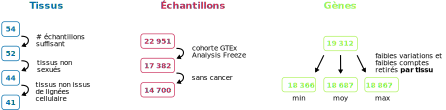
\includegraphics[width=1\textwidth]{img/chap2/chap2_filtre_donnees.pdf}
    % \includesvg[scale=.5]{img/chap2/chap2_filtre_donnees.svg}
    \caption{Ensemble des filtres appliqués sur les différentes données et impact sur les données utilisées pour la construction ultérieure des réseaux de co-expression.}
    \label{figure:data_filters}
    % \caption{Nombre d'échantillons disponibles par tissu et par tranche d'âge de 10 ans dans les données de GTEx.}
\end{figure}



Par ailleurs, tous les donneurs n'ont pas pu être prélevés pour l'ensemble des 54 tissus et ce sont en moyenne 23,4 tissus qui ont été prélevés (v8). Certains tissus ont été priorisés lors des biopsies : tissu adipeux (sous-cutané), artère tibiale, cœur (ventricule gauche), poumon, muscle (squelettique), nerf tibial, peau (exposée au soleil), thyroïde, sang complet. Parmi les différents tissus biopsiés, il est à noter que certains sont issus d'un même organe et on a ainsi 31 organes biopsiés pour 54 tissus biopsiés en tout.

% \todo[inline]{Un Sankey diagramme des tissus avec col 1 = SMTS, col 2 = SMTSD, col 3 = tranche d'age à 10 ans}


\subsection{Sélection des tissus}

Le vieillissement est un phénomène dont les altérations moléculaires sont linéaires avec le temps, dont les dommages cellulaires sont super-linéaires \citeB{Todhunter2018}, et où la mortalité associée augmente de façon exponentielle passée 20 ans \citeB{Finch2016}. Afin de faciliter la détection de ces altérations grâce à l'analyse de co-expression différentielle, on s'est donc dans un premier temps concentré sur une sélection de tranches d'âges très contrastées. Les échantillons sélectionnés sont issus de donneurs entre 20 et 30 ans pour la tranche qu'on nommera "\textbf{jeune}", et entre 60 et 70 ans pour la tranche qu'on nommera "\textbf{âgée}". Les données de GTEx ne comportent toutefois pas un nombre d'échantillons similaire pour chacune de ces tranches du fait de la mortalité plus importante chez les personnes âgées que les personnes jeunes (principalement des décès par traumatisme chez les jeunes plutôt que par maladie chronique ou maladie liée à l'âge chez les âgés). Un premier filtre de notre pré-traitement restreint donc la sélection des tissus à ceux comportant au minimum 50 échantillons dans chacune des tranches d'âge, ce qui n'est pas le cas de la Vessie (20) et le Rein - Médulla (3). Ce nombre d'échantillons permet d'assurer un bon compromis entre des réseaux de co-expression de gènes robustes (donc non sensibles à des valeurs aberrantes) et la perte de plus de tissus à étudier dans cette analyse multidimensionnelle qu'on souhaite effectuer \citeB{Liesecke2019}.

Tous les tissus restant n'étaient pas nécessairement adaptés à l'étude globale du vieillissement chez l'humain. Ainsi on a retiré tous les tissus liés à un seul sexe : Trompes de Fallope, Col de l'utérus, Utérus, Vagin, Sein, Ovaire, Prostate, Testicule. À ce retrait s'ajoute celui des échantillons de lignées cellulaires (dérivées ou non de tissus eux conservés) car non représentatifs du vieillissement biologique : Cellules - Lymphocytes transformés par EBV, Cellules - Fibroblastes cultivés, Cellules - Lignée cellulaire de leucémie (CML). 


\begin{figure*}[h]
    \centering
    \includegraphics[width=1\textwidth]{img/chap2/chap2_sample_count_by_tissu.png}
    \caption{Nombre d'échantillons disponibles par tissu et par tranche d'âge de 10 ans dans les données de GTEx.}
    \label{figure:sample_count_by_tissu}
\end{figure*}


\subsection{Filtre des échantillons}


En plus de ces sélections de tissus, certains échantillons ont directement nécessité une filtration afin de prévenir de potentiels biais. Ainsi, seuls les échantillons répondant au critère d'inclusion dans la cohorte "GTEx Analysis Freeze" ont été retenus en premier lieu (Figure \ref{figure:data_filters}. Cette cohorte atteste que les échantillons n'étaient pas issus de donneurs ayant des liens de parenté ou de donneurs avec des critères d'exclusion, par exemple des donneurs avec des duplications/délétions chromosomiques, affectés d'un syndrome tel que défini par la base de données OMIM \citeB{Hamosh2005} (ce qui n'inclue pas les maladies liées au vieillissement), ou encore ayant effectué une chirurgie de ré-assignation sexuelle. 

\begin{figure}[hb]
    \centering
    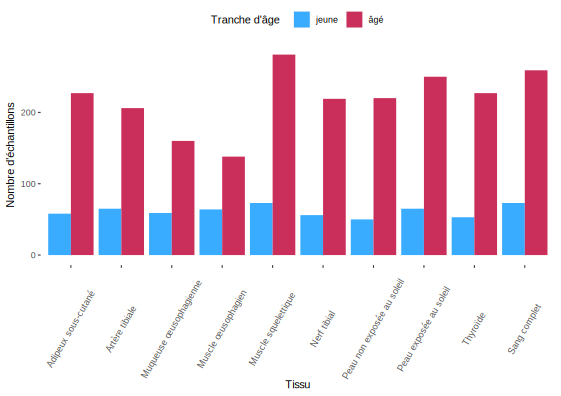
\includegraphics[width=1\textwidth]{img/chap2/chap2_sample_count_by_tissu_after_filter.pdf}
    \caption{Nombre d'échantillons disponibles par tissu dans les tranches d'âge jeune (20-30) et âgé (60-70) après filtration selon la cohorte et le statut cancéreux.}
    \label{figure:sample_count_by_tissu_after_filter}
\end{figure}

Par ailleurs, l'expression des tissus tumoraux a montré, dans des études préalables, des modèles d'expression génétique différents de ceux non tumoraux \citeB{Tang2017}. Par conséquent, les échantillons de ces donneurs ont également été supprimées ici ainsi que les échantillons dont le statut cancéreux était inconnu. La répartition finale des échantillons par tissu et par tranche d'âge est visible en Figure \ref{figure:sample_count_by_tissu_after_filter}.


\subsection{Filtre sur les gènes}

On a considéré comme base dans cette étude uniquement les gènes codants pour une protéine (d'après GENCODE 26) sur les autosomes. Pour continuer à éviter l'influence du sexe, on a également limité les gènes des gonosomes à ceux du chromosome X. Afin de limiter l'ajout de biais d'origine technique, on a également exclu les gènes dont le compte de lecture (en anglais \textit{count}) était inférieur à 6 dans la totalité des échantillons \citeB{Rocke2001}. Les gènes n'ayant aucune variation se sont vu retirés du jeu de données car leur apport à la co-expression aurait était nul et leur conservation aurait entraîné l'utilisation de ressources inutile. Ces filtres ayant été appliqués par tissu, le nombre de gènes restant varie d'un tissu à un autre avec en moyenne 18687 gènes (Figure \ref{figure:data_filters}).



\subsection{Correction des facteurs confondants}

À l'instar de l'analyse d'expression différentielle, l'analyse de co-expression différentielle nécessite des données biaisées au minimum pour une construction de réseau de qualité. Ces biais (ou facteurs confondants) peuvent être tant techniques que biologiques et vont entraîner une augmentation de la variation de façon artificielle. Le risque est alors de détecter une différence artificielle et de l'assumer comme expérimentalement pertinente alors qu'elle est en fait due aux biais. Dans le cas de la co-expression plus spécifiquement, ces bais peuvent entraîner des corrélations erronées mais qui semblent crédibles entre certains gènes. Elles altèrent alors la construction du réseaux de co-expression et par la suite la détection des modules qui se base sur un découpage en modules via les corrélations. Ainsi, il est essentiel de corriger ces facteurs confondants au préalable de l'utilisation du package R GWENA \citeB{Lemoine2021Dec} sur les données comme on va le faire par la suite.

La complexité de la correction des facteurs confondant réside dans leur suppression sans pour autant altérer la distribution des données ou supprimer le signal expérimental d'intérêt, ici les variations dans le transcriptome dûs à l'âge. Il est également important avec l'utilisation de GWENA de veiller à ce que la correction n'altère pas la topologie d'invariance d'échelle qu'on retrouve dans les données de transcriptomique après construction d'un réseau de co-expression. En effet, cela invaliderait la méthode de détection des modules.
% Comme précisé en \ref{subsubsection:microarray_props_and_normalisation} et \ref{subsubsection:rnaseq_props_and_normalisation}, chaque technologie de séquençage a un premier ensemble de normalisations spécifique à elle, limitant ainsi un premier ensemble de biais spécifiques. 

% \todo{Je me demande si ces 2 paragraphes plus haut ne devraient pas finir en intro de thèse}

La base de données GTEx n'échappe pas aux biais et a même été étudiée sur le plan de la contamination \citeB{Nieuwenhuis2020}.
Malgré le progrès de techniques ciblées sur des facteurs confondants connus comme l'effet de lot, l'effet de centre de prélèvement, le sexe, le poids, etc., celles-ci ne sont pas capables de corriger pour des facteurs peu explicites ou diffus comme la classe sociale, l'alimentation, la façon de manipuler des techniciens, etc. La correction par composante principale (CP) vise à répondre à ce type de problématique et a montré de bons résultats selon une évaluation par validation de voies de signalisation au sain de modules détectés. \citeB{Parsana2019}. Elle a également montré de meilleurs résultats que d'autres méthodes telles que que la régression multiple, le taux exonique, ou encore le numéro d'intégrité d'ARN (\textit{RNA integrity number}, ou RIN). Fait important pour la co-expression en particulier, cette méthode conserve la propriété d'invariance d'échelle des données.

Cependant cette correction va également corriger l'âge qui est notre variable d'intérêt. Afin de conserver cette information tout en ayant un effet de correction par CP sur les autres facteurs confondants, on a donc ajusté la méthode estimant le nombre $n$ de CP par lequel corriger les jeux de données. Au lieu d'utiliser une procédure de permutation \citeB{Buja1992Oct}, l'estimation de $n$ s'est faite en deux étapes :
\begin{itemize}
    \item Un test de corrélation de chaque gène avec l'âge associé à chaque échantillon (donc patient) en fonction de différent $n$ PC corrigées donne une liste de gènes significativement associés à l'âge.
    \item Cette liste de gènes par $n$ PC corrigées est ensuite croisée avec deux bases de données de gènes connus comme étant associés au vieillissement : GenAge \citeB{DeMagalhaes2004} et Digital Aging Atlas \citeB{Craig2015}. Y sont alors compté le nombre de gènes significatifs recoupés.
\end{itemize}
Finalement, le $n$ de PC à corriger retenu est celui où le nombre de gènes significatifs est le plus haut dans chaque base de données. En cas de divergence de ce $n$ entre les bases de données, on a sélectionné la valeur la plus basse de $n$ afin de ne pas risquer de corriger l'âge (Table \ref{table:nb_PC_corr_and_samples_by_tissue}).


\begin{table}[h!]
% \resizebox{\textwidth}{!}{
\centering
\begin{tabular}{llll}
\multirow{2}{*}{\textbf{Tissu}} & \multirow{2}{*}{\textbf{\begin{tabular}[c]{@{}l@{}}Nombre de CP \\ corrigées\end{tabular}}} & \multicolumn{2}{l}{\textbf{Nombre d'échantillons}} \\ \cline{3-4} 
                                &                                                                                             & \textbf{Jeune}            & \textbf{Âgé}           \\ \hline
Adipeux sous-cutané             & 1                                                                                           & 58                        & 227                    \\
Artère tibiale                  & 3                                                                                           & 65                        & 206                    \\
Muqueuse œusophagienne          & 1                                                                                           & 59                        & 160                    \\
Muscle œusophagien              & 3                                                                                           & 64                        & 138                    \\
Muscle squelettique             & 5                                                                                           & 73                        & 281                    \\
Nerf tibial                     & 4                                                                                           & 56                        & 219                    \\
Peau non exposée au soleil      & 4                                                                                           & 50                        & 220                    \\
Peau exposée au soleil          & 3                                                                                           & 65                        & 250                    \\
Thyroïde                        & 3                                                                                           & 53                        & 227                    \\
Sang complet                    & 1                                                                                           & 73                        & 259                   
\end{tabular}
% }
\caption{Résumé du nombre de composantes utilisées pour effectuer la correction de l'expression par tissu, ainsi que le nombre d'échantillons inclus dans chacun pour les deux plages d'âge.}
\label{table:nb_PC_corr_and_samples_by_tissue}
\end{table}

% \todo[inline]{Idée de figure : remplacer cette table ou en touts cas la partie nb composantes par un ensemble de mini histogrames avec les deux bdd en un, et en facet pour chaque tissu.}



% \subsection{Détections des modules }
\subsection{Construction du réseau, détection des modules et co-expression différentielle}

Une fois les données pré-traitée, nous avons généré un réseau de co-expression de gènes indépendamment sur chacun des 10 tissus et tranche d'âge à l'aide du package GWENA \citeB{Lemoine2021Dec}. Les paramètres spécifiés étaient ceux par défaut de la fonction \verb+build_net+ à l'exception de la corrélation qui était elle basée sur Spearman et du seuil d'ajustement de la loi de puissance fixé à 0.8. Dans chaque réseau de tissu, on a ensuite détecté le nombre de modules via la fonction \verb+detect_modules+ selon un seuil de coupe de l'arbre hiérarchique identique dans chaque tissu et une taille de module minimale fixée à 20 gènes. Chaque ensemble de modules a ensuite été testé à l'aide de la fonction \verb+compare_conditions+ par tissu entre les deux tranches d'âges pour identifier les modules préservés, modérément préservés et non préservés avec le vieillissement.

% \subsection{Co-expression différentielle et }





% \section{Construction des réseaux par tissu et détection des modules}
% \section{Isolement des modules d'intérêt}
\section{Résultats}

% Suite à ce pré-traitement des données, on a pu s'attacher 
% \subsection{Construction des réseaux par tissu et détection des modules}
% En utilisant les données d'expression qui ont passé les contrôles de qualité décrits ci-dessus, nous avons généré un réseau de co-expression de gènes indépendamment sur chacun des 10 tissus et tranche d'âge à l'aide du package GWENA. 
% La loi de puissance associée à chacun des réseau a retourné des \textalpha{} 
% \begin{table}[h]
% \centering
% \begin{tabular}{lll}
% \textbf{Tissu}             & \textbf{\textalpha{}  Jeune} & \textbf{ \textalpha{}  Âgé} \\ \hline
% Adipeux sous-cutané        & 14             & 14           \\
% Artère tibiale             & 6              & 9            \\
% Muqueuse œusophagienne     & 14             & 16           \\
% Muscle œusophagien         & 12             & 18           \\
% Muscle squelettique        & 6              & 8            \\
% Nerf tibial                & 7              & 12           \\
% Peau non exposée au soleil & 8              & 8            \\
% Peau exposée au soleil     & 10             & 10           \\
% Thyroïde                   & 16             & 12           \\
% Sang complet               & 18             & 14          
% \end{tabular}
% \end{table}
% Dans chaque réseau, on a ensuite détecté le nombre de modules optimaux (à seuil de coupe identique de l'arbre hiérarchique) avec une variation de leur nombre visible en Figure \ref{figure:repartition_genes_modules_tissus} entre couples tissus / tranche d'âge.

\begin{figure}[!hb]
    \centering
    \includegraphics[width=1\textwidth]{img/chap2/chap2_repartition_genes_modules_tissus.png}
    \caption{Répartition des gènes (en échelle log10) pour chaque tissu entre les deux tranches d'âge jeune (bleu) et âgée (rouge)}
    \label{figure:repartition_genes_modules_tissus}
\end{figure}

\subsection{Répartition des gènes en fonction de la tranche d'âge et du tissu}

La répartition des gènes entre les modules est hétérogène, tant entre les tranches d'âge qu'entre les tissus (Figure \ref{figure:repartition_genes_modules_tissus}), avec une moyenne à 26 modules tout confondu (25.2 pour les âgés et 26.8 pour les jeunes). Le module 0 présent sur la figure regroupe les gènes sans association à un module. Celui-ci est quasi systématiquement plus grand dans la tranche âgée que jeune, à l'exception des tissus de la thyroïde et du sang complet. Les tissus où cet écart est le plus creusé sont ceux disposant du plus grand nombre de modules dans la tranche d'âge jeune. Ces résultats sont cohérents avec la tendance à la perte de co-expression constatée dans les tranches d'âge âgées \citeB{Southworth2009} : la perturbation des voies de signalisation au cours du vieillissement entraîne une diminution de la co-expression entre gènes de ces voies.

\subsection{Modules spécifiques du vieillissement et recoupement inter-tissus}

% Le but étant de rechercher les origines des gènes associés au vieillissement 
Le but étant de rechercher des origines communes au vieillissement entre tous les tissus, on a ensuite effectué une étape de co-expression différentielle intra tissu. La tranche d'âge jeune a été prise pour référence, c’est-à-dire que le test indiquera si chaque module détecté dans la tranche d'âge jeune est préservé, modérément préservé, non préservé, ou non concluant. Les résultats ont été résumés en Table \ref{table:modules_status_all_tissues}. 

On y constate que certains tissus tendent à avoir proportionnellement moins de modules préservés lors du vieillissement. Avec moins de 50 \% de préservation on retrouve notamment le muscle œsophagien et squelettique, ainsi que de la peau exposée au soleil et la thyroïde. À cela s'ajoute que la peau exposée au soleil et le muscle squelettique sont les deux tissus ayant le plus de modules non préservés proportionnellement à leur nombre de modules.

\begin{table}[!ht]
\resizebox{\textwidth}{!}{
\begin{tabular}{llllllllll}
\multirow{2}{*}{\textbf{Tissu}} & \multicolumn{2}{l}{\textbf{Préservé}} & \multicolumn{2}{l}{\textbf{Modérement préservé}} & \multicolumn{2}{l}{\textbf{Non préservé}} & \multicolumn{2}{l}{\textbf{Non concluant}} & \textbf{Total} \\ \cline{2-10} 
                                & \textbf{\#}       & \textbf{\%}       & \textbf{\#}             & \textbf{\%}            & \textbf{\#}         & \textbf{\%}         & \textbf{\#}          & \textbf{\%}         & \textbf{\#}    \\ \hline
Adipeux sous-cutané             & 12                & 67              & 4                       & 22                   & 0                   & 0                 & 2                    & 11               & 18             \\
Artère tibiale                  & 13                & 57              & 8                       & 35                   & 1                   & 4                 & 1                    & 4                & 23             \\
Muqueuse œusophagienne          & 3                 & 25              & 8                       & 67                   & 1                   & 8                 & 0                    & 0                & 12             \\
Muscle œusophagien              & 9                 & 43              & 6                       & 29                   & 0                   & 0                 & 6                    & 29               & 21             \\
Muscle squelettique             & 14                & 40              & 13                      & 37                   & 5                   & 14                & 3                    & 9                & 35             \\
Nerf tibial                     & 35                & 71              & 9                       & 18                   & 1                   & 2                 & 4                    & 8                & 49             \\
Peau non exposée au soleil      & 36                & 90              & 4                       & 10                   & 0                   & 0                 & 0                    & 0                & 40             \\
Peau exposée au soleil          & 10                & 48              & 8                       & 38                   & 2                   & 10                & 1                    & 5                & 21             \\
Thyroïde                        & 12                & 48              & 8                       & 32                   & 1                   & 4                 & 4                    & 16               & 25             \\
Sang complet                    & 9                 & 64              & 4                       & 29                   & 0                   & 0                 & 1                    & 7                & 14              
\end{tabular}
}
\caption{Nombre (\#) et ratio (\%) de modules par statut de préservation selon chaque tissu.}
\label{table:modules_status_all_tissues}
\end{table}

%  0.64|                   0.29|            NA|           0.07|

Afin d'observer des similarités de mécanismes du vieillissement entre ces différents tissus, on a dans un premier temps regardé si des gènes communs existaient entre les modules modérément préservés (MP) et non  préservés (NP). Le diagramme UpSet visible en Figure \ref{figure:upset_intersection_genes_tissu_unpres_modpres} permet de constater le faible recouvrement entre les gènes contenus dans les modules MP et NP. Ce diagramme révèle également que le maximum de tissus avec des gènes communs est 5. Ce chiffre est à mettre en contraste avec le fait que les modules créés par GWENA pour un même tissu ne sont pas chevauchant. Un gène classé dans un module ne sera donc pas également classé dans un autre et on aurait pu espérer une intersection au maximum de taille 10 étant donné qu'on dispose de 10 tissus. 

\todo{Peut être retravailler la figure pour la découper selon le nombre de tissus à l'intersection (de 1 à 5)}
\begin{landscape}
\begin{figure}[p]
  \centering
  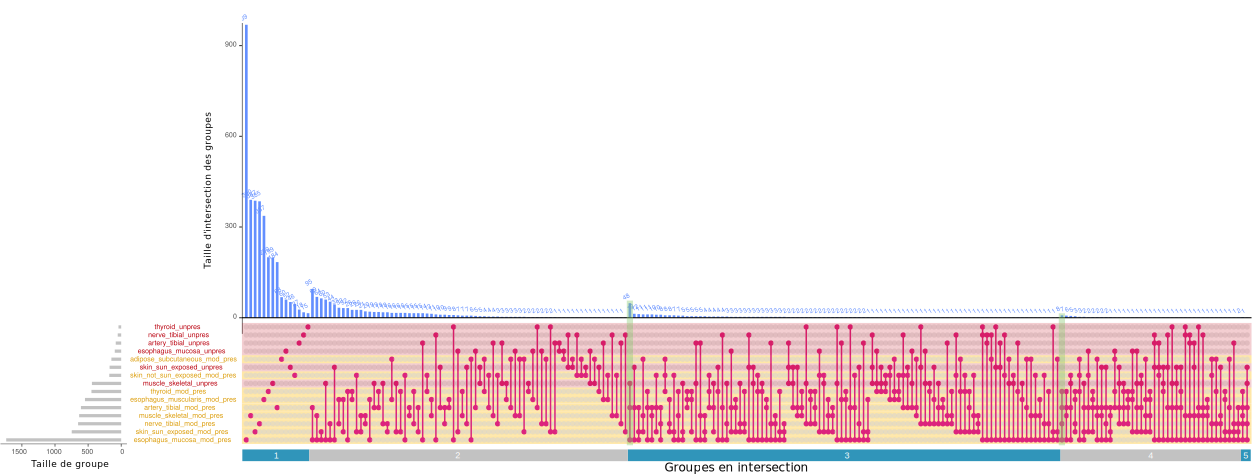
\includegraphics[width=1.5\textheight]{img/chap2/chap2_upset_genes_unpres_modpres_by_tissue.pdf}
%   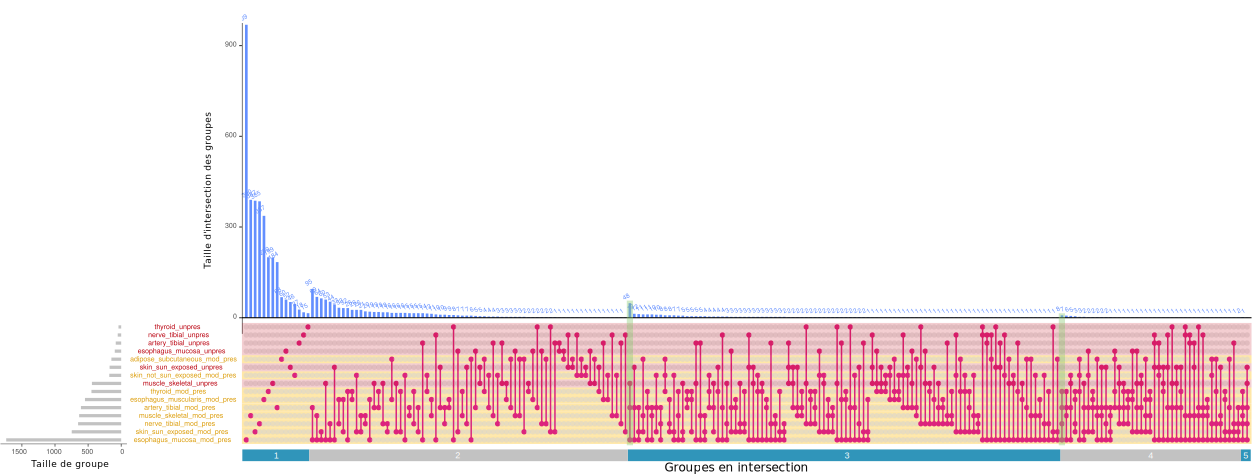
\includegraphics[width=1\textheight]{img/chap2/chap2_upset_genes_unpres_modpres_by_tissue.pdf}
  \caption{Intersections entre tous les jeux de gènes pour chaque couple tissu / statut de préservation. Le diagramme Upset est une représentation qui vise à remplacer une visualisation par diagramme de Venn, ce dernier n'étant pas adaptée à la représentation de plus de 5 catégories \citeB{Lex2014}. La matrice d'intersection (en orange) indique quel couple tissu / statut est considéré dans l'intersection (rose si pris en compte, gris si non) et quels sont les autres tissus dans cette intersection (ligne rose). L'histogramme des tailles de groupe (gris) à gauche de la matrice indique le nombre total de gène contenu dans le couple tissu / statut en ligne. L'histogramme des tailles d'intersection indique le nombre de gènes contenu dans l'intersection indiquée en matrice d'intersection pour cette colonne.}
  \label{figure:upset_intersection_genes_tissu_unpres_modpres}
\end{figure}
\end{landscape}

% \begin{figure}[p]
%     \begin{adjustbox}{addcode={
%         \begin{minipage}{0.98\width}}{
%             \caption{Intersections entre tous les jeux de gènes pour chaque couple tissu / statut de préservation. Le diagramme Upset est une représentation qui vise à remplacer une visualisation par diagramme de Venn, ce dernier n'étant pas adaptée à la représentation de plus de 5 catégories \citeB{Lex2014}. La matrice d'intersection (en orange) indique quel couple tissu / statut est considéré dans l'intersection (rose si pris en compte, gris si non) et quels sont les autres tissus dans cette intersection (ligne rose). L'histogramme des tailles de groupe (gris) à gauche de la matrice indique le nombre total de gène contenu dans le couple tissu / statut en ligne. L'histogramme des tailles d'intersection indique le nombre de gènes contenu dans l'intersection indiquée en matrice d'intersection pour cette colonne.}
%             \label{figure:upset_intersection_genes_tissu_unpres_modpres}
%         \end{minipage}},rotate=90,center}
%         % \includesvg[scale=.5]{img/chap2/chap2_upset_genes_unpres_modpres_by_tissue.svg}
%         % \includesvg[width=1\textheight]{img/chap2/chap2_upset_genes_unpres_modpres_by_tissue.svg}
%         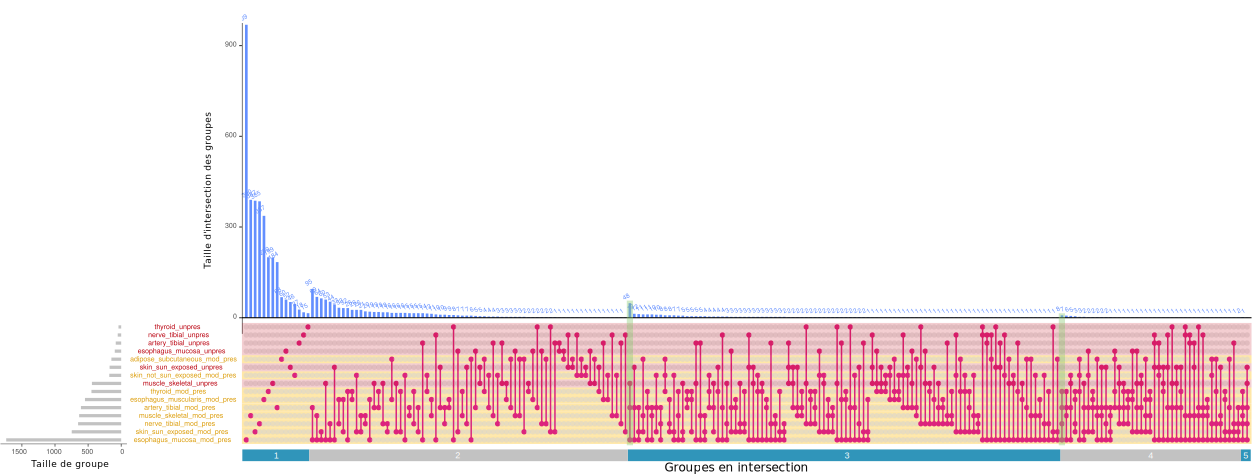
\includegraphics[width=1\textheight]{img/chap2/chap2_upset_genes_unpres_modpres_by_tissue.pdf}
%     \end{adjustbox}
% \end{figure}


% D'un point de vue taille des intersections, les probabilités de présence de cha
En plus de ce nombre maximal de tissus présent dans une intersection, certains tissus vont se retrouver plus fréquemment dans ces intersections en raison de leur nombre de modules MP/NP et/ou de modules contenant plus de gènes (Table \ref{table:modules_status_all_tissues}).
% Pour compléter, les probabilités de recoupement de gènes ne sont pas identique comme en témoignent les ratios de statut de préservation en table \ref{table:modules_status_all_tissues}. Certains tissus tendent à avoir plus de modules MP/NP et/ou des modules de plus grande taille (avec le plus de gènes), favorisant alors leur probabilité de recoupement avec d'autres tissus. 
Ainsi, les modules MP de la muqueuse œsophagienne regroupent 1750 gènes et tendent à se positionner dans plus d'intersection que la moyenne. Une séparation est toutefois visible entre les deux types de statut MP et NP dans les intersections au-delà de 2 tissus et avec un minimum de trois gènes.

\subsection{Répartition des phénomènes communs liés au vieillissement dans plusieurs tissus}

Pour mieux comprendre les fonctions physiologiques communes en jeu et pouvant être impliquées dans le vieillissement, les intersections de plus de 3 tissus et ayant au moins 5 gènes ont été enrichies via GWENA. Comme visible en Annexe \ref{annexe:chap_2_genes_intersect_enrichments} dans les tables des enrichissements obtenus, 5 intersections n'ont pas donné d'enrichissement significatif malgré un nombre de gènes équivalent à d'autres intersections avec enrichissement. Les 18 autres intersections ont quant à elles retourné des fonctions physiologiques (Gene Ontology \citeB{Ashburner2000}, CORUM \citeB{Ruepp2008}) et voies d'activation (KEGG \citeB{Kanehisa2019}, REACTOME \citeB{Fabregat2016}, WikiPathways\citeB{Slenter2018}) connues comme faisant partie du vieillissement global, ou de manifestations spécifiques à plusieurs tissus. Ainsi on retrouve, dans ces intersections de modules peu ou pas préservés dans la tranche âgée, des fonctions associées à l'homéostasie, la régulation de la transcription, la gestion des dérivés réactifs de l'oxygène, l'inflammation, etc. (Table \ref{table:intersection_aging_global_phenomenons} et Figure \ref{figure:revigo_resume_4_enrich}). La muqueuse œsophagienne bien qu'ayant un nombre de gènes plus élevé que les autres tissus ne se retrouve pas sur-représentée dans ces phénomènes observés. Cela indique donc que la majorité de ses gènes se trouvent dans les intersections de faible taille, tant en gènes qu'en nombre de tissus recoupés. Le sang complet, le tissu adipeux sous-cutané et la peau non exposée au soleil sont eux les tissus les moins présents dans ces intersections avec des phénomènes liés au vieillissement. Le sang complet est notablement absent des intersections avec des phénomènes liés à la coagulation. Les tissus ayant un fort renouvellement (voir en Table \ref{table:tissu_telomere_effet}) que sont les épithéliums (peau exposée au soleil, artère tibiale, muqueuse œsophagienne) sont porteurs d'un grand nombre de phénomènes, ainsi que la thyroïde et le muscle squelettique. 


\begin{table}[]
\resizebox{\textwidth}{!}{
\begin{tabular}{@{}lllllllllll@{}}
\rotatebox{90}{\textbf{Muqueuse œusophagienne}}   & \rotatebox{90}{\textbf{Artère tibiale}}                      & \rotatebox{90}{\textbf{Thyroïde}}                 & \rotatebox{90}{\textbf{Muscle squelettique}}      & \rotatebox{90}{\textbf{Peau exposée au soleil}}   & \rotatebox{90}{\textbf{Muscle œusophagien}}       & \rotatebox{90}{\textbf{Nerf tibial}}              & \rotatebox{90}{\textbf{Peau non exposée au soleil}} & \rotatebox{90}{\textbf{Adipeux sous-cutané}}      & \rotatebox{90}{\textbf{Sang complet}}             & \textbf{Phénomène du vieillissement observé}       \\ \midrule
\cellcolor[HTML]{F8A102} & \cellcolor[HTML]{F8A102}            &                          & \cellcolor[HTML]{F8A102} &                          &                          &                          & \cellcolor[HTML]{F8A102}   &                          &                          & Homéostasie                               \\
                         & \cellcolor[HTML]{F8A102}            & \cellcolor[HTML]{F8A102} &                          &                          & \cellcolor[HTML]{F8A102} &                          &                            &                          &                          & Régulation de la transcription            \\
\cellcolor[HTML]{F8A102} &                                     & \cellcolor[HTML]{F8A102} & \cellcolor[HTML]{F8A102} &                          &                          &                          &                            &                          &                          & Dérivés réactifs de l'oxygène - peroxydes \\
                         &                                     & \cellcolor[HTML]{F8A102} &                          & \cellcolor[HTML]{F8A102} & \cellcolor[HTML]{F8A102} & \cellcolor[HTML]{F8A102} &                            &                          &                          & Dérivés réactifs de l'oxygène - dGTP      \\
                         &                                     & \cellcolor[HTML]{F8A102} &                          &                          &                          &                          & \cellcolor[HTML]{F8A102}   & \cellcolor[HTML]{F8A102} &                          & Inflammation                              \\
                         &                                     &                          &                          & \cellcolor[HTML]{F8A102} & \cellcolor[HTML]{F8A102} & \cellcolor[HTML]{F8A102} &                            &                          &                          & Désamination                              \\
\cellcolor[HTML]{F8A102} & \cellcolor[HTML]{F8A102}            &                          &                          &                          &                          & \cellcolor[HTML]{F8A102} &                            &                          &                          & Coagulation - plaquettes                  \\
\cellcolor[HTML]{F8A102} & \cellcolor[HTML]{F8A102}            & \cellcolor[HTML]{F8A102} &                          &                          &                          & \cellcolor[HTML]{F8A102} &                            &                          &                          & Coagulation - global                      \\
\cellcolor[HTML]{F8A102} & \cellcolor[HTML]{F8A102}            &                          & \cellcolor[HTML]{F8A102} &                          &                          &                          &                            &                          &                          & Méthylation - folate, B12, selenium       \\
                         &                                     &                          & \cellcolor[HTML]{F8A102} & \cellcolor[HTML]{F8A102} &                          &                          &                            & \cellcolor[HTML]{F8A102} &                          & Méthylation - déméthylase                 \\
\cellcolor[HTML]{F8A102} & \cellcolor[HTML]{F8A102}            &                          & \cellcolor[HTML]{F8A102} &                          &                          &                          &                            &                          & \cellcolor[HTML]{F8A102} & Altération de la MEC                      \\
                         &                                     & \cellcolor[HTML]{F8A102} &                          & \cellcolor[HTML]{F8A102} & \cellcolor[HTML]{F8A102} &                          &                            &                          &                          & Anomalie du taux de glutamine             \\
\cellcolor[HTML]{F8A102} &                                     &                          &                          & \cellcolor[HTML]{F8A102} &                          &                          & \cellcolor[HTML]{F8A102}   &                          &                          & Synthèse de pigment (dont mélanine)      \\
\cellcolor[HTML]{F8A102} & \cellcolor[HTML]{F8A102}            & \cellcolor[HTML]{F8A102} & \cellcolor[HTML]{F8A102} &                          &                          &                          &                            &                          &                          & Anomalie du taux de fer                   \\
\midrule
8                        & 7                                   & 7                        & 6                        & 5                        & 4                        & 4                        & 3                          & 2                        & 1                        & \textbf{Total}                   
\end{tabular}
}
\caption{Phénomènes connus dans le vieillissement et observés dans les intersections de modules MP et NP pour chaque tissu. Les modules MP et NP ont été joints par tissus et les tissus ont été ordonnés par nombre décroissant de phénomènes du vieillissement présent. MEC : Matrice extra-cellulaire.}
\label{table:intersection_aging_global_phenomenons}
\end{table}

% \begin{table}[]
% \resizebox{\textwidth}{!}{
% \begin{tabular}{@{}lllllllllll@{}}
% % \toprule
% \rotatebox{90}{\textbf{Adipeux sous-cutané }}      & \rotatebox{90}{\textbf{Artère tibiale }}           & \rotatebox{90}{\textbf{Muqueuse œusophagienne }}   & \rotatebox{90}{\textbf{Muscle œusophagien }}       & \rotatebox{90}{\textbf{Muscle squelettique }}      & \rotatebox{90}{\textbf{Nerf tibial }}              & \rotatebox{90}{\textbf{Peau non exposée au soleil }} & \rotatebox{90}{\textbf{Peau exposée au soleil }}   & \rotatebox{90}{\textbf{Thyroïde }}                 & \rotatebox{90}{\textbf{Sang complet }}             & \textbf{Phénomène du vieillissement observé}       \\ \midrule
%                          & \cellcolor[HTML]{F8A102} & \cellcolor[HTML]{F8A102} &                          & \cellcolor[HTML]{F8A102} &                          & \cellcolor[HTML]{F8A102}   &                          &                          &                          & Homéostasie                               \\
%                          & \cellcolor[HTML]{F8A102} &                          & \cellcolor[HTML]{F8A102} &                          &                          &                            &                          & \cellcolor[HTML]{F8A102} &                          & Régulation de la transcription            \\
%                          &                          & \cellcolor[HTML]{F8A102} &                          & \cellcolor[HTML]{F8A102} &                          &                            &                          & \cellcolor[HTML]{F8A102} &                          & Dérivés réactifs de l'oxygène - peroxydes \\
%                          &                          &                          & \cellcolor[HTML]{F8A102} &                          & \cellcolor[HTML]{F8A102} &                            & \cellcolor[HTML]{F8A102} & \cellcolor[HTML]{F8A102} &                          & Dérivés réactifs de l'oxygène - dGTP      \\
% \cellcolor[HTML]{F8A102} &                          &                          &                          &                          &                          & \cellcolor[HTML]{F8A102}   &                          & \cellcolor[HTML]{F8A102} &                          & Inflammation                              \\
%                          &                          &                          & \cellcolor[HTML]{F8A102} &                          & \cellcolor[HTML]{F8A102} &                            & \cellcolor[HTML]{F8A102} &                          &                          & Désamination                              \\
%                          & \cellcolor[HTML]{F8A102} & \cellcolor[HTML]{F8A102} &                          &                          & \cellcolor[HTML]{F8A102} &                            &                          &                          &                          & Coagulation - plaquettes                  \\
%                          & \cellcolor[HTML]{F8A102} & \cellcolor[HTML]{F8A102} &                          &                          & \cellcolor[HTML]{F8A102} &                            &                          & \cellcolor[HTML]{F8A102} &                          & Coagulation - global                      \\
%                          & \cellcolor[HTML]{F8A102} & \cellcolor[HTML]{F8A102} &                          & \cellcolor[HTML]{F8A102} &                          &                            &                          &                          &                          & Méthylation - folate, B12, selenium       \\
% \cellcolor[HTML]{F8A102} &                          &                          &                          & \cellcolor[HTML]{F8A102} &                          &                            & \cellcolor[HTML]{F8A102} &                          &                          & Méthylation - déméthylase                 \\
%                          & \cellcolor[HTML]{F8A102} & \cellcolor[HTML]{F8A102} &                          & \cellcolor[HTML]{F8A102} &                          &                            &                          &                          & \cellcolor[HTML]{F8A102} & Altération de la MEC                      \\
%                          &                          &                          & \cellcolor[HTML]{F8A102} &                          &                          &                            & \cellcolor[HTML]{F8A102} & \cellcolor[HTML]{F8A102} &                          & Anomalie du taux de glutamine             \\
%                          &                          & \cellcolor[HTML]{F8A102} &                          &                          &                          & \cellcolor[HTML]{F8A102}   & \cellcolor[HTML]{F8A102} &                          &                          & Synthèse de pigement (dont mélanine)      \\
%                          & \cellcolor[HTML]{F8A102} & \cellcolor[HTML]{F8A102} &                          & \cellcolor[HTML]{F8A102} &                          &                            &                          & \cellcolor[HTML]{F8A102} &                          & Anomalie du taux de fer                   \\ 
% \end{tabular}
% }
% \caption{Phénomènes connus dans le vieillissement et observés dans les intersections de modules MP et NP pour chaque tissu. Les modules MP et NP ont été joints par tissus pour une meilleure lisibilité.}
% \label{table:intersection_aging_global_phenomenons}
% \end{table}

\begin{figure}[ht]
    \centering
    \includegraphics[width=1\textwidth]{img/chap2/chap2_revigo_resume_4_enrich.png}
    \caption{Exemple de résumé des enrichissements sur GO pour 4 des intersections par carte proportionnelle. Chaque ensemble de GO terme partageant une ontologie parente commune (selon un score de similarité) est groupé sous une même couleur. Chaque carte présente ici un phénomène connu dans le vieillissement : A. Homéostasie (GO \textit{Biological Process}), B. Régulation de la transcription (GO \textit{Biological Process}), C. Dérivés réactifs de l'oxygène (GO \textit{Molecular Function}), D. Inflammation (GO \textit{Biological Process}) }
    \label{figure:revigo_resume_4_enrich}
\end{figure}

Des anomalies phénotypiques ont été relevées (via enrichissement sur HPO \citeB{Kohler2019}) et présentent un lien plus ou moins direct avec les altérations physiologiques précédemment relevées. Aux anomalies du taux de fer détectés dans les fonctions physiologiques coïncident ainsi des phénotypes d'anémie (déficience en taux de globules rouges ou en concentration d'hémoglobine) ou de défaut de coagulation avec hémorragies diverses (épistaxis, saignement gingival, menstruations hors cycle, hémorragie cérébrale). De même, les tissus présentant une altération de la matrice extra-cellulaire (MEC) ont été associés avec des taux élevés de protéine C-réactive et d'anomalies de la fonction exocrine du pancréas ainsi que de malabsorption des lipides et ce qui en découle (stéatorrhée, pancréatite, thrombose veineuse). Ces résultats confirment le lien entre vieillissement et dérèglement progressif de l'homéostasie entrainant en cascade des pathologies de trouble de la coagulation \citeB{Franchini2006,Kario1993} et de la dégradation des lipides circulants \citeB{Yamamoto2014, Hirschfield2003}. Cependant d'autres résultats semblent moins intuitifs comme dans le cas de pathologies liées au sexe (azoospermie, maladie d'hérédité gonosomale) relevées parallèlement à la déméthylation dans le tissu adipeux, le muscle squelettique et la peau non exposée au soleil. Ces informations, en l'absence d'erreur technique, semblent continuer de montrer la complexité des relations entre pathologies et vieillissement.

Enfin, on a exploré le vieillissement et son phénomène de perturbation de la régulation de la transcription en évaluant l'enrichissement d'éléments de régulation (MiRTarBase \citeB{Chou2018}, TRANSFAC \citeB{Matys2006}). L'intersection présentant des phénomènes de coagulation globale est ainsi fortement enrichi en micro ARN (miARN). Ceux-ci contiennent notamment des miARN associés aux 3 gènes de la génération de fibrinogène FGA, FGB, FGG comme détectés lors du chapitre précédent. Quelques autres intersections. Deux facteurs de transcription (FT), HNF1A et HNF1B, sont également significatifs bien que normalement exprimés dans le foie. Cela s'explique par la production de facteurs de la coagulation (dont FGA, FGB, FGG) dans celui-ci et un effet connu de l'altération de production de ces facteurs dans le cadre d'une perturbation de l'expression de HNF1A et HNF1B \citeB{Costa2003}. L'intersection associée à l'inflammation quant à elle ne présente qu'un seul miARN agissant ici sur RSAD2, IFI44, OASL, et EPSTI1 présents dans l'intersection. RSAD2 et OASL sont également connus pour être stimulé par des interférons de type I (\textalpha{} et \textbeta{}) qui ont entre autres IRF1 (pour \textit{interferon related factor 1}) pour FT \citeB{Schoggins2011}. Ce facteur IRF1 fait par ailleurs parti de la liste des FT détectés dans cette intersection. On y trouve un large panel d'autres membres de la famille d'IRF (de 1 à 9 à l'exception d'IRF6) dont l'implication dans l'inflammation s'exerce tant dans la réaction innée qu’acquise \citeB{Frisch2020}. Mais tous les FT détectés via enrichissement n'étaient pas des IRF. Bien que n'étant pas directement liés à la régulation des interférons, STAT2 est présent dans la voie de signalisation des interférons \textalpha{} et \textbeta{} détecté plus tôt (R-HSA-909733). Le dernier FT identifié, FOXP1, n'est quant à lui pas contenu dans cette voie, mais agit sur l'engagement des cellules souches mésenchymateuses et la sénescence au cours du vieillissement \citeB{Infante2018} et sur de la régulation d'autres cytokines, l'interleukine 1 et 12 d'après UniprotKB (Q9H334).

\subsection{Les variation de co-expression dans l'intersection liée à l'inflammation}

L'inflammation systémique chronique de faible intensité est une des marques connues du vieillissement \citeB{Lopez-Otin2013, Franchini2006}. La complexité des mécanismes d'immunité et d'inflammation rend ce phénomène particulièrement difficile à étudier et les publications actuelles tendent donc à cibler peu d'acteurs en même temps (gène, protéine, miARN, etc.) et à se concentrer sur des contextes très précis \citeB{Franceschi2017}. Bien qu'apportant un niveau de preuve inférieur à toute validation expérimentale, les réseaux de co-expression de gènes permettent de comprendre bien plus d'acteurs. À titre d'exemple, on a souhaité ici détailler le cas de l'intersection de gènes associés à l'inflammation lors du vieillissement (Figure \ref{figure:revigo_resume_4_enrich}.D).

\begin{figure}[p]
    \centering
    \includegraphics[width=1\textwidth]{img/chap2/chap2_graphs_intersection_plot_adipo_skinnosun_thyr.png}
    \caption{Réseaux de co-expression des gènes de l'intersection associée au phénomène d'inflammation lors du vieillissement entre les deux tranches d'âge. Le réseau est filtré à 0.95 de dissimilarité (sur une échelle de 0 à 1) pour des questions de lisibilité et 3 tissus sont présentés : tissu adipeux, peau non exposée au soleil et thyroïde.}
    \label{figure:graphs_intersection_plot_adipo_skinnosun_thyr}
\end{figure}

Les variations de motif dans la co-expression sont bien souvent la première cause de non-préservation des modules. Des changements de score de centralité, des modifications de gène pivot (\textit{hub gene}), des suppressions totales de signal sont bien souvent à l'origine de cette différence de topologie détectée entre les modules à l'aide de la co-expression différentielle \citeB{Ritchie2016,Zhang2005a}. Cet effet se manifeste de plusieurs façons dans le cas de l'intersection sur l'inflammation comme visible en figure \ref{figure:graphs_intersection_plot_adipo_skinnosun_thyr}. Bien que la variation de la co-expression ne soit pas identique entre tous les tissus qui forment cette intersection, on observe des acteurs communs. Le gène RSAD2 précédemment mis en avant comme gène simulé par le FT IRF1 et un mARN devient ainsi un gène pivot dans la condition âgée selon le classement de score de centralité. Cependant, les sources de progression dans le classement selon la centralité divergent selon le tissu. Dans le tissu adipeux on constate que c'est dû à un renfort de la co-expression entre RSAD2 et IF44 associé à une perte partielle de co-expression globale par CMPK2, gène pivot dans la condition jeune. Dans la peau non exposée au soleil, on constate un renfort global de la co-expression avec toutefois une centralisation vers RSAD2. Une augmentation localisée entre OAS2 et OASL est également à noter. Enfin, dans la thyroïde, c'est une déconnexion entre HERC6 et OAS2 au profit de RSAD2 qui le rend gène pivot dans la condition âgée. Si cette réorganisation de la co-expression vers RSAD2 aurait pu être issue d'une contribution d'IRF1 ou tout autre IRF étant donné les informations précédentes, des analyses complémentaires ont précisé qu'aucun des IRF détectés comme FT auparavant n'était présent dans le module où se trouve RSAD2 (jeune comme âgé). L'origine de la variation de RSAD2 et OAS2/OASL pourrait donc être d'une autre nature qu'une modification de la transcription d'un ou plusieurs FT.


\subsection{Cas particulier : le vieillissement spécifique à la peau}

Si le vieillissement partage des mécanismes et altérations communes à travers plusieurs tissus, il existe parallèlement des altérations spécifiques à certains tissus. Bien que ne permettant pas l'enrichissement global de la compréhension du vieillissement, ces altérations locales nécessitent de s'y intéresser afin de prévenir et prendre en charge les pathologies qui s'y rattachent. En étudiant les intersections ne présentant pas d'enrichissements liés aux mécanismes communs du vieillissement et en tenant compte des tissus inclus, on peut ainsi étudier l'impact du vieillissement spécifique du tissu.
% La peau est un des organes dont l'intégrité est la plus susceptible d'être mise à mal par le vieillissement en raison de son exposition directe avec l'environnement extérieur. 
% Le premier facteur de vieillissement extrinsèque est le photo-vieillissement dont les effets sont cumulatifs avec le temps \citeB{Farage2008}. Il se caractérise majoritairement pas une exposition aux UVs (UVA et UVB) qui vont induire des détériorations des fibres de collagène et d'élastine dans la peau. À noter également, des altérations de la matrice extra-cellulaire entre l'épiderme et le derme qui sont les deux couches composant la peau \citeB{Rogowski-Tylman2016}. 

\begin{figure}[hb]
    \centering
    \includegraphics[width=1\textwidth]{img/chap2/chap2_revigo_resume_enrich_skin.png}
    \caption{Résumé des enrichissements sur GO par carte proportionnelle de l'intersection peau exposée au soleil, peau non exposée au soleil et muqueuse œsophagienne. Chaque ensemble de GO terme partageant une ontologie parente commune (selon un score de similarité) est groupé sous une même couleur.}
    \label{figure:revigo_resume_melanine}
\end{figure}

% Une intersection faite de la peau exposée au soleil, la peau non exposée au soleil et la muqueuse œsophagienne fait état dans notre cas d'un tel type de photo-vieillissement. 
Une intersection faite de la peau exposée au soleil, la peau non exposée au soleil et la muqueuse œsophagienne fait état dans notre cas d'un tel type de vieillissement. 
Elle est en effet composée principalement d'enrichissements sur des fonctions physiologiques directement liées à la synthèse et régulation de mélanine comme exposé en Figure \ref{figure:revigo_resume_melanine}. 
% Ce pigment synthétisé par les mélanocytes à partir d'une oxydation de la tyrosine joue un rôle majeur de lutte contre les dégâts provoqués par les UV \citeB{Bettley1965}. 
C'est le gène TYR, impliqué dans cette synthèse qu'on trouve dans le réseau de co-expression de notre intersection qui entraîne notamment cet enrichissement. Il est détecté comme gène pivot (score de centralité) dans chacun des tissus et chacune des tranches d'âge (Figure \ref{figure:graphs_intersection_melanine}), attestant ainsi de son rôle majeur dans la régulation de la mélanogénèse. On constate qu'il est lié dans la condition jeune par une relation forte (dissimilarité < 0.8 en moyenne) avec un autre gène, SLC24A5. Ce gène est connu pour coder pour un échangeur de cations (sodium, potassium, calcium) de façon générale et a été plusieurs fois soupçonné d'une contribution à la régulation de la mélanogénèse \citeB{Zhang2019,Ginger2008}. C'est notamment à lui que se rattachent les enrichissements de type \textit{secondary metabolite biosynthetic process}. 
% Aucune confirmation de son rôle de régulateur partiel de la production de mélanine n'a été faite chez l'homme malgré sa mise en évidence chez la souris . 
% Contrairement à la tyrosinase produite par TYR qui se trouve dans les mélanosomes, la protéine NCKX5 produite par SLC24A5 est localisée dans les mitochondries. 
% dans le cas des deux tissus de peau, mais pas dans la muqueuse œsophagienne
À ces deux gènes s'ajoute une relation de chacun avec CLEC12B dans le cas des deux tissus de peau et pas de la muqueuse œsophagienne. Ce gène appartient à la famille des récepteurs de lectine de type C qui jouent un rôle essentiel dans l'immunité et l'homéostasie à laquelle contribue la mélanine localement. La fonction de CLEC12B elle-même reste cependant encore mal caractérisée malgré la présence d'un motif d'inhibition basé sur la tyrosine d'un immunorécepteur dans son domaine intracellulaire. Ceci lui permettrait donc de recruter SHP-1/SHP-2 \citeB{Hoffmann2007Aug, Tone2019}, deux phosphatases suspectées d'avoir un rôle dans la progression des mélanomes \citeB{Zhang2013}. 

La Figure \ref{figure:graphs_intersection_melanine} permet de constater que la relation TYR/SLC24A5 tend à augmenter avec l'âge dans la peau exposée ou non au soleil. Si l'augmentation est très marquée la peau non exposée au soleil, elle est bien moindre dans la peau non exposée. Ces résultats coïncident avec l'augmentation de la production de mélanine constatée chez la personne âgée pour compenser la diminution globale de la densité de mélanocytes \citeB{Gilchrest1979}. À l'inverse, la co-expression de CLEC12B avec SLC24A5 et TYR tend à diminuer avec l'âge, ainsi que l'intégralité de la co-expression de l'intersection.

La muqueuse œsophagienne elle semble interagir plus étroitement avec deux autres gènes, GML et ALX1 avec toutefois une interaction notable de la peau exposée au soleil avec ALX1 également. ALX1 est un gène jouant un rôle dans la migration cellulaire dans les structures craniofaciale lors du stade embryon, tandis que la fonction de GML est peu connu en dehors d'une potentielle contribution dans la voie d'activation de l'apoptose via p53 en cas de dommage à l'ADN. Comme visible en Figure \ref{figure:graphs_intersection_melanine}, la relation entre ces gènes ainsi qu'avec le gène TYR tend à diminuer dans la tranche âgée, qu'il s'agisse de la muqueuse œsophagienne comme de la peau exposée au soleil.


Si la mélanine est connue comme pigment et protectrice contre les UV, il est \citeB{Tolleson2005}



\begin{figure}[p]
    \centering
    \includegraphics[width=1\textwidth]{img/chap2/chap2_graphs_intersection_melanine.png}
    \caption{Réseaux de co-expression des gènes de l'intersection associée à la surproduction de mélanine lors du vieillissement entre les deux tranches d'âge. Le réseau est filtré à 0.99 de dissimilarité (sur une échelle de 0 à 1) pour des questions de lisibilité et 3 tissus sont présentés : muqueuse œsophagienne, peau non exposée au soleil et peau exposée au soleil.}
    \label{figure:graphs_intersection_melanine}
\end{figure}


\section{Discussion}

\subsection{La susceptibilité des tissus aux variations liées au vieillissement}

Le vieillissement peut être vu comme une imbrication de multiples phénomènes qui découlent d'une dérégulation du fonctionnement physiologique ou d'une réponse à cette dérégulation. En prenant en compte le système dans sa quasi-intégralité, les réseaux de co-expression permettent d'acquérir de nouvelles connaissances au-delà d'acteurs transcriptomiques individuels connus. Les variations au cours du temps des relations de co-expression entre gènes sont alors les témoins d'autant de voies d'activations qui s'altèrent. Leur suivi et mise en contraste au travers de la co-expression différentielle sont donc à leur tour un moyen supplémentaire de comprendre le déroulé des altérations \citeB{Sharan2006, Southworth2009}. En comparant ces dernières entre de multiples tissus, il est possible d'en déduire des mécanismes communs au vieillissement, et à l'inverse ceux spécifiques. Dans cette étude, on s'est donc attaché étudier ce vieillissement d'un point de vue multi-dimensionnel en comparant les réseaux issus de multiples tissus, et ce, entre deux tranches d'âge extrêmes. 

Si le vieillissement tend à perturber de nombreuses fonctions physiologiques, il semble cependant que peu de gènes soient impactés ou impactant dans ce processus. Ainsi, comme cela a pu être observé auparavant \citeB{Avelar2019}, une minorité de gènes varie significativement entre les deux conditions (modules NP) et une proportion légèrement plus grande varie modérément (modules MP) (Figure \ref{figure:upset_intersection_genes_tissu_unpres_modpres}). 
Ils suffisent pourtant à représenter une large majorité des phénomènes connus du vieillissement : perte d'homéostasie, instabilité génomique, inflammation, dérivés réactifs de l'oxygène, etc. (Table \ref{table:intersection_aging_global_phenomenons} et Figure \ref{figure:revigo_resume_4_enrich}). 
Si leur répartition est inégale entre les tissus, ceux en portant le plus coïncident avec les tissus ayant un fort taux de renouvellement \citeB{Armanios2012, Barker2010, Leblond1956} (Table \ref{table:intersection_aging_global_phenomenons}) à l'exception dans notre cas de la thyroïde dont le renouvellement cellulaire minimal est de 8 ans \citeB{Coclet1989Dec}. 
% La présence de cette dernière est probablement due à d'autres phén
% Dans le cas de cette dernière, d'autre
% Les fonctions qu'ils encodent sont toutefois les 
% Nombre de phénomènes connus du vieillissement \citeB{Lopez-Otin2013} sont par ailleurs inégalement répartis en leur sein selon les différents tissus.
% Ce faisant, on a pu dans un premier temps observer les marques du vieillissement \citeB{Lopez-Otin2013} dans les diverses intersections détectées associée à l'âge par notre analyse de co-expression différentielle : perte d'homéostatie, instabilité génomique, inflammation, dérivés réactifs de l'oxygène, etc. (Table \ref{table:intersection_aging_global_phenomenons} et Figure \ref{figure:revigo_resume_4_enrich}).
% On a cependant pu constater la disparité de présence de ces marques du vieillissement entre tous les organes. Une majorité de gènes ne varient ainsi pas significativement lors du vieillissement comme cela a pu être observé auparavant \citeB{Avelar2019} (Figure \ref{figure:upset_intersection_genes_tissu_unpres_modpres}). 
% La disparité observée dans leur répartition dans toutes les intersections tient notamment 
% Certains tissus cependant sont plus sujets que d'autres à ces variations et coïncident le plus souvent avec les tissus ayant un fort taux de renouvellement \citeB{Armanios2012, Barker2010, Leblond1956} (Table \ref{table:intersection_aging_global_phenomenons}) avec l'exception dans notre cas de la thyroïde. 
Malgré une évidence des modifications que subit le système endocrinien avec le vieillissement, l'impact de celui-ci sur la thyroïde reste peu documenté hors pathologies graves \citeB{Faggiano2011Sep}. En effet, les altérations endocrines thyroïdiennes (hypo ou hyperthyroïdies) sont souvent associées à un vieillissement "naturel" de la personne \citeB{Cooper2004Dec}. Il est donc présomptueux ici de s'essayer à trouver une cause d'autant de marques du vieillissement sans plus d'information. Pourtant, les indices d'un rôle de la thyroïde sur la longévité s'accumulent ces dernières années \citeB{Garasto2017Jul,Arosio2020Sep}. Renforcer les connaissances sur les altérations de la fonction thyroïdienne chez la personne âgée semble donc une voie intéressante pour l'amélioration de la durée de vie chez l'homme.


\subsection{La variation de la réponse inflammatoire issue du vieillissement}

L'inflammation chronique de faible intensité est une caractéristique majeure du vieillissement qu'on nomme en anglais "\textit{inflammaging}" \citeB{Franceschi2014Jun} et dont la complexité limite encore les connaissances à son sujet \citeB{Franceschi2017}. Si l'inflammation est un mécanisme bénéfique dans la réponse aigüe et temporaire à un pathogène, elle se retrouve délétère dans le cas du vieillissement malgré une faible intensité car elle est persistante. Ce phénomène assumé comme étant un précurseur de plusieurs autres phénomènes du vieillissement \citeB{Lopez-Otin2013} s'est retrouvé ici plutôt exprimé dans le tissu adipeux, la peau non exposée au soleil, ainsi que la thyroïde. Les enrichissements fonctionnels sont venu préciser cette composante de l'inflammation comme une réponse à une réaction virale. En cause, de nombreux régulateurs d'interférons de type I significativement enrichis malgré leur absence de l'intersection. Ceci s'explique à contrario par la présence de nombreux gènes de réponse aux interférons, stimulés en temps normal par la présence d'ARN ou ADN viral.

Les interférons de type I (IFN-I) sont des cytokines regroupant tous les interférons à l'exception des IFN-\textgamma{} et dont les interférons majoritaires sont les IFN-\textalpha{} et IFN-\textbeta{}. Ces IFN-I ont pour rôle, dans la réponse inflammatoire classique, d'entraver à la fois la réplication du virus et les cellules hôtes infectées. Pour cela, un large panel de gènes de réponse aux interférons, dont ceux détectés ici, est induit avec différents objectifs : interférer avec le trafic intracellulaire des vésicules, limiter la stabilité et la traduction des ARNm viraux, et entraîner une apoptose de la cellule au besoin via la voie d'activation de la protéine p53\citeB{Frisch2020}. Cependant l'intervention de ce mécanisme antiviral dans le cadre du vieillissement est encore mal compris. Une hypothèse prometteuse est que des éléments transposables, plus particulièrement les LINE-1 (\textit{long interspersed nuclear elements}) se retrouvent non réprimés avec l'âge en raison d'une dégradation des acteurs de leur répression (ex : des petits ARN ou \textit{small RNA} (smRNA) en anglais) \citeB{Kreiling2017Jan, DeCecco2019Feb, Frisch2020}. Ces LINE-1 codent alors pour diverses transcriptases inverses et autres protéines de rétro-transposition qui vont déclencher la réponse anti-virale associée à une sénescence \citeB{QiujingYu2015May}. S'il est admis que cette réponse varie de la "normale" antivirale, il reste toutefois difficile de comprendre comment les gènes antiviraux se comportent dans ce cadre non-viral \citeB{Frisch2020} et la raison pour laquelle des marqueurs de la sénescence sont produits.

Dans le cadre de notre étude, on a constaté que le gène antiviral RSAD2 induit par les interférons officie comme gène pivot de co-expression. Dans le cas de la peau non exposée au soleil, il collabore également étroitement avec deux autres gènes antiviraux de la famille OAS : OAS2 et OASL. Les gènes OAS ont déjà été auparavant associés à une réponse de type IFN-I induite par la sénescence et plus particulièrement l'accumulation d'ADN dans la cellule \citeB{DeCecco2019Feb} qui est une composante délétère du vieillissement. Concernant RSAD2, aucun lien direct chez l'humain n'a été mis en avant à ce jour, seulement chez la souris \citeB{Ma2020Mar}. La protéine produite par RSAD2 est connue pour limiter la réplication de l'ADN viral ou de l'ARN double brin viral bien que le mécanisme par lequel elle opère n'est pas entièrement clair \citeB{Fitzgerald2011Jan}. En plus d'être un potentiel marqueur de cette accumulation d'ADN liée aux éléments transposables, RSAD2 pourrait donc être un potentiel gène candidat pour le développement de médicaments anti-âge.

% La limite entre réaction inflammatoire mesurée et délétère est mince. Un retour à l'équilibre est donc primordial pour un vieillissement en bonne santé. 

% Les interferons induisent une production de plusieurs gènes impliqués dans la réponse virale
% En temps normal, cela 
% Dans le cadre du vieillissement, la production d'interférons est induite par les LINEs et ne semble pas passer par les IRF classique car ils ne retrouvent pas présents dans ce module associé à l'inflammation
% Parallèlement, RSAD2 est un gène induit en temps normal par les IFN-I au même titre que d'autre gènes, mais semble présenter ici un profil différent dans la condition âgée de ce qu'on pourrait attendre dans une stimulation par IFN-I classique.
% Pas exactement le meme pathway de trigger ?
% Si les gènes OAS ont déjà auparavant été associés à une réponse de type IFN-I induite par la sénescence, ce n'est pas le cas de RSAD2 \citeB{DeCecco2019Feb} qui semble par ailleurs dans notre cas être plus co-exprimé dans la condition âgée que les gènes OAS.

% Le role de base des interferons :  bind to specific receptors on target cells, which leads to expression of proteins that will prevent the virus from producing and replicating its RNA and DNA.

%  Our understanding of how a tailored switch from homeostasis to a strong receptor-dependent response is coordinated remain limited



% Les preuves d'implicatLes preuves d'implication des cytokines et plus précisément des interferons de type I dans le vieillissement sont nombreuses \citeB{Frisch2020}.

% ion des cytokines et plus précisément des interferons de type I dans le vieillissement sont nombreuses \citeB{Frisch2020}.
% Le

% Si leur rôle est effectivement lié à cette fonction dans le fonctionnement "normal" de l'humain,
% Cependant ces enrichissements sont issus

% Si les LINE ne sont pas directement ciblables par des thérapies, le triplet RSAD2/OAS2/OASL 

% Une étude de l'intersection de gènes caractéristiques de l'inflammation chronique de faible intensité a 

\subsection{L'altération de la régulation des mélanocytes et de la mélanogénèse avec l'âge}

Au-delà des manifestations communes du vieillissement, chaque tissu est affecté de façon plus spécifique dans sa physiologie. L'altération avec l'âge de la mélanogénèse est un de ces changements qu'on retrouve en toute logique uniquement dans les tissus disposant de mélanocytes. La peau est l'organe en disposant du plus grand nombre et se retrouve ainsi d'autant plus affecté par cette altération avec l'âge. Dans notre intersection liée à la mélanogénèse, l'hyper-pigmentation connue dans le vieillissement \citeB{Hakozaki2016Sep} s'est retranscrite par l'augmentation de la co-expression entre TYR et SLC24A5, respectivement catalyseur et régulateurs de la production d'eumélanine \citeB{Cullinane2011Oct, Ginger2008}, dans la peau exposée ou non au soleil. L'augmentation nettement plus grande dans la peau non exposée au soleil était toutefois inattendue étant donné que l'hyper-pigmentation a plutôt été relevée dans les peaux exposées au soleil en raison de la stimulation de la mélanogénèse par les UV \citeB{Gilchrest1979}. 
% Dans la muqueuse œsophagienne, autre tissu présent dans cette intersection, cette co-expression de TYR avec SLC24A5 à l'inverse diminue. Peu d'études existent sur le contenu en mélanocytes de ce tissu et leur rôle en son sein reste donc mal compris en dehors des mécanismes déjà connus dans la peau comme la réduction des dérivés réactifs de l'oxygène ou la fixation de certaines molécules organiques et ions métalliques \citeB{Tolleson2005}.

En plus d'une co-expression entre TYR et SLC24A5, une forte co-expression de CLEC12B a été montrée dans les deux tissus de peau. Une investigation de ce gène a révélé que peu d'information est connue sur ses fonctions et son implication dans la mélanogénèse. Des résultats préliminaires conséquents ont toutefois montré sa capacité à recruter les phosphorylases SHP-1/SHP-2 via son domaine ITIM \citeB{Sormani2019}, enzymes notamment connues pour leur implication dans la pigmentation dans le syndrome LEOPARD \citeB{Motegi2015}. Ce nouveau gène impliqué dans la pigmentation de la peau coïncide ainsi avec les estimations d'un plus grand nombre de gènes contribuant au spectre de pigmentation que ceux actuellement connus et majeurs comme MC1R \citeB{Parra2004Nov}. 
Contrairement à la co-expression entre TYR et SLC24A5, CLEC12B tend à perdre sa synergie avec l'âge. Avec l'âge, CLEC12B tend à perdre sa synergie avec TYR et SLC24A5. L'inactivation de CLEC12B ayant démontré une diminution de la pigmentation dans un modèle de peau humaine reconstruite \citeB{Sormani2019}, on peut alors se demander si ce gène ne serait pas impliqué dans le phénomène de dépigmentation global de la peau lors du vieillissement (phénomène parallèle à l'hyper-pigmentation locale). Plus précisément, CLEC12B serait impliqué dans les voies d'inhibition de la prolifération des mélanocytaire par le biais de p53/p21/p27 \citeB{montaudie2019} et on pourrait envisager alors que la diminution de la densité de mélanocytes avec l'âge serait en partie dû à la diminution de co-expression de CLEC12B avec TYR et SLC24A5.


% % Si CLEC12B est co-exprimé dans les deux tissus de peau, ce n'est pas le cas dans la muqueuse œsophagienne. On y retrouve plutôt deux autres gènes, ALX1 et GML, co-exprimés avec le couple SLC24A5 / TYR, et dont la co-expression diminue fortement avec l'âge. 
% % Associé à la diminution de co-expression entre SLC24A5 et TYR
% % La muqueuse œsophagienne n'étant pas exposée aux UV, la production de mélanine n'est pas stimulée par ce biais et les autres acteurs de sa stimulation semblent donc diminuer d'efficacité avec le vieillissement.
% Dans la muqueuse œsophagienne, autre tissu présent dans cette intersection, cette co-expression de TYR et SLC24A5 avec CLEC12B est bien plus faible en comparaison. 
% % Dans la muqueuse œsophagienne, autre tissu présent dans cette intersection, cette co-expression de TYR avec SLC24A5 à l'inverse diminue et CLEC12B se retrouve peu co-exprimé en comparaison. 
% La présence de la muqueuse œsophagienne dans cette intersection contenant des tissus de peau s'explique par ailleurs par la présence dans chacun d'eux d'un épithélium squameux stratifié, dérivé de la crête neurale \citeB{delaPava1963}.
% Peu d'études existent sur le contenu en mélanocytes de ce tissu et leur rôle en son sein reste donc mal compris en dehors des mécanismes déjà connus dans la peau comme la réduction des dérivés réactifs de l'oxygène ou la fixation de certaines molécules organiques et ions métalliques \citeB{Tolleson2005}. 
% % ###########
% La muqueuse œsophagienne, 3ème tissu présent dans l'intersection, 
La muqueuse œsophagienne et la peau étant toutes deux des tissus dotés d'un épithélium squameux stratifié dérivé de la crête neurale \citeB{delaPava1963}, il est cohérent de les retrouver au sein d'une même intersection. Pierson et al. ont d'ailleurs montré la proximité de leur expression dans leur étude du jeu de données GTEx \citeB{Pierson2015}. S'il est commun que la peau soit étudiée pour son contenu en mélanocytes, il est beaucoup moins courant que le contenu en mélanocytes de la muqueuse œsophagienne soit étudié. Le rôle de ce type cellulaire dans ce tissu reste ainsi encore mal compris en dehors des parallèles avec les mécanismes déjà connus dans la peau comme la réduction des dérivés réactifs de l'oxygène ou la fixation de certaines molécules organiques et ions métalliques \citeB{Tolleson2005}. 
% Peu d'études existent sur le contenu en mélanocytes de ce tissu et leur rôle en son sein reste donc mal compris en dehors des mécanismes déjà connus dans la peau comme la réduction des dérivés réactifs de l'oxygène ou la fixation de certaines molécules organiques et ions métalliques \citeB{Tolleson2005}. 

Dans cette intersection côté muqueuse œsophagienne donc, la co-expression de TYR et SLC24A5 avec CLEC12B fait place à une co-expression croisée de TYR et SLC24A45A avec ALX1 et GML. 
GML est un homologue des protéines de membrane ancrées de type glycosyl-phosphatidylinositol(GPI), mais dont la fonction encore inconnue est suspectée d'être liée à l'apoptose et la régulation du cycle cellulaire \citeB{Furuhata1996Nov}. Il a été constaté que son expression tend à ralentir la progression des cellules cancéreuses de l'œsophage et à augmenter la sensibilité des cellules cancéreuses à certaines chimiothérapies \citeB{Catalano2001May}. 
De son côté, ALX1 est un facteur de transcription impliqué dans la régulation de gènes liés au développement embryonnaire et à la migration cellulaire \citeB{Dee2013Jan}. Il a été détecté comme sous exprimé chez des embryons de souris irradié entrainant un retard de pigmentation de l'épithélium rétinien. 
Pris ensemble, ces gènes pourraient donc être soupçonnés d'être à l'origine de la régulation de la prolifération des mélanocytes dans la muqueuse œsophagienne, bien qu'aucune direction de régulation ne puisse être extrapolée de nos réseaux de co-expression en tant que tel. En revanche, on peut avancer que si une telle régulation existe, elle est perturbée avec le vieillissement d'après la diminution notable de la co-expression entre TYR et SLC24A5 (donc contraire à l'évolution de la co-expression dans la peau) coïncidant avec la forte diminution de leur co-expression avec ALX1 et GML ainsi qu'entre eux deux. 
Ces altérations et les fonctions pour lesquelles codent ces gènes évoquent logiquement le développement de mélanomes qui sont parmi les pathologies associées au vieillissement et où les fonctions de régulation de la prolifération des mélanocytes par ALX1 et GML pourraient entrer en jeu. Toutefois, le mélanome œsophagien reste une pathologie rare, même si la fréquence des mélanomes œsophagiens d'origine métastatique est plus élevée que celle des mélanomes œsophagiens d'origine primitive. Il reste donc compliqué d'évaluer l'impact de la diminution de co-expression de ALX1 et GML ainsi que SLC24A5 et TYR dans le vieillissement de la muqueuse œsophagienne. Si des études sont menées ultérieurement sur ces gènes ou sur le contenu en mélanocytes de la muqueuse œsophagienne, elles pourront potentiellement donner de nouvelles perspectives à ces résultats.
% s'il est plus fréquent dans le cas d'un mélanome d'origine métastatique que d'origine primaire œsophagienne. Il reste donc compliqué d'évaluer l'impact de la diminution de co-expression de ALX1 et GML ainsi que SLC24A5 et TYR dans le vieillissement de la muqueuse thyroïdienne.

% ###########




% La muqueuse œsophagienne n'étant pas exposée aux UV, la production de mélanine n'est pas stimulée par ce biais et les autres acteurs de sa stimulation semblent donc diminuer d'efficacité avec le vieillissement comme en témoigne la diminution de co-expression entre TYR et SLC24A5. Ce changement coïncide avec la forte diminution de co-expression de ALX1 et GML avec TYR et SLC24A5 entre la tranche jeune et la tranche âgée.

% GML est un homologue des protéines de membrane ancrées de type glycosyl-phosphatidylinositol(GPI), mais dont la fonction encore inconnue est suspectée d'être liée à l'apoptose et la régulation du cycle cellulaire \citeB{Furuhata1996Nov}. Il a notamment été constaté que son expression tend à ralentir la progression des cellules cancéreuses de l'œsophage et à augmenter la sensibilité des cellules cancéreuses à certaines chimiothérapies \citeB{Catalano2001May}. 
% % On peut également ajouter que ses protéines similaires avec un ancrage via glycosyl-phosphatidylinositol (GPI) ont été associées aux mélanomes \citeB{Food1994Jan} et plus spécifiquement à la mélanogénèse \citeB{Okamura2017Feb}. 

% De son côté, ALX1 est un facteur de transcription impliqué dans la régulation de gènes liés au développement embryonnaire et à la migration cellulaire \citeB{Dee2013Jan}. Il a notamment été détecté comme sous exprimé chez des embryons de souris irradié entrainant un retard de pigmentation de l'épithélium rétinien. 
% % Chose notable chez ces embryons, la quantification de la protéine issue de ALX1 n'avait pas montré de diminution, suggérant un.
% Prises ensemble, ces informations 
% La contribution de ces 
% % Prises ensemble, ces informations tendent à suggérer une voie de stimulation de la mélanogénèse parallèle à celle stimulée par les UV. Elle diffère de cette dernière par l'implication des gènes ALX1 et GML visant semble-t-il à user de la fonction de 





% L'interaction de GML et ALX1 avec TYR et SLC24A5 ainsi que leur variation significative dans des expériences impliquant la mélanogénèse tend à confirmer l'existence d'une voie de régulation de la production de mélanine parallèle à celle stimulée par les UV. 
% La suppression de leur co-expression avec l'âge est quant à elle intéressante vis à vis de l'augment




% % L'évolution avec l'âge de la co-expression de CLEC12B avec TYR et SLC24A5 semble cependant différer de celle entre ces deux derniers 
% % La contribution similaire de CLEC12B n'a cependant pas été publiée à ce jour bien que des résultats préliminaires étendus aient prouvé sa capacité à recruter SHP-1/SHP-2 ainsi qu'une dépigmentation dans un modèle de peau humaine reconstruite dans le cas d'une inactivation de CLEC12B \citeB{Sormani2019}. Une éventuelle relation vis-à-vis de SLC45A2 n'a quant à elle jamais été étudiée. 



% % Dans notre intersection liée à la mélanogénèse, le gène TYR connu pour son rôle de catalyseur majeur de l'eumélanine s'est révélé être un hub gêne, témoignant encore une fois de son 

% % tyrosinaseinhibition, blocking melanosome transfer, inhi-bition of tyrosinase glycosylation, increasingtyrosinase turnover, and blocking inflamma-tion are c



% % la mélanogénèse et plus largement des mélanocytes a donc été l'objet de nombreuses études. On peut distinguer toutefois les études se 
% % la mélanine pourrait protéger les cellules du stress oxydatif au delà de la simple photoprotection
% % Sous le terme de mélanine se regroupent en fait deux molécules pincipa
% % La mélanine est un dérivé de l'oxydation d'une tyrosine couplée à des intermédiaires 
% % Les mélanocytes sont un type cellulaire présent majoritairement dans l'épiderme en raison de leur rôle premier : la protection contre les effets délétères des UV. La mélanine qu'ils produisent


% % D'autres tissus sont é

% % Si les mélanocytes se retrouvent 
% % D'autres tissus accueillent également des mélanocytes. Outre les tissus pigmentés comme l'uvée dans l'œil, des mélanocytes sont présents dans plusieurs tissus dérivés de la crête neurale. La muqueuse œsophagienne est l'un de ces tissus.






% Chaque tissu subit le vieillissement à une vitesse différente. 
% Dans cette étude on s'est intéressés dans un second temps aux tissus les plus exposés avec l'extérieur car ils sont plus susceptibles de porter des marques du vieillissement en raison du stress qu'ils reçoivent. 
% % Ceux les plus exposés avec l'extérieur se retrouvent ainsi plus susceptibles de vieillir prématurément en raison du stress qu'ils reçoivent. 
% Ils sont ainsi les plus susceptibles de développer des pathologies ou de laisser passer des agents pathogènes.
% % Chaque organe subit le vieillissement de différentes manières.
% Dans la peau, ce vieillissement est d'autant plus accentué qu'elle est particulièrement exposée aux facteurs extérieurs et notamment au photo-vieillissement. 
% % Le photo-vieillissement dû aux UV est ainsi une composante majeure de son vieillissement prématuré du fait du stress et des mutations qu'il induit \citeB{Fisher2002}. 
% Pour se protéger du stress induit, elle dispose de mélanocytes, type cellulaire chargé entre autre de produire de la mélanine. 
% L'objectif de cette molécule est de limiter l'impact des UV, des dérivés réactifs de l'oxygène, et des radicaux libres. En complément, elle est également capable de séquestrer les ions métalliques et de lier certains médicaments et molécules organiques \citeB{Tolleson2005}. 
% % La première étape de sa synthèse part d'une tyrosine 
% % Sa production débute par la catalyse d'une tyrosine pa
% % Produite à partir de tyrosine
% % Pour produire la mélanine
% % La production de la mélanine débute à partir d'une tyrosine dont la 
% La production de la mélanine débute par la catalyse d'une tyrosine en L-Dopaquinone par une tyrosinase codée par le gène TYR. Dans notre analyse, le gène SLC45A2 se retrouve fortement co-exprimé avec celui-ci, suggérant un rôle de contributeur dans cette synthèse comme cela a été soupçonné auparavant \citeB{Cullinane2011Oct, Ginger2008}. 
% La contribution similaire de CLEC12B n'a cependant pas été publiée à ce jour bien que des résultats préliminaires étendus aient prouvé sa capacité à recruter SHP-1/SHP-2 ainsi qu'une dépigmentation dans un modèle de peau humaine reconstruite dans le cas d'une inactivation de CLEC12B \citeB{Sormani2019}. Une éventuelle relation vis-à-vis de SLC45A2 n'a quant à elle jamais été étudiée. 

% La muqueuse œsophagienne possède, elle aussi, des mélanocytes même si leur rôle est encore mal compris, d'où la présence de ce tissu dans cette intersection.
% % La muqueuse œsophagienne possède, elle aussi, des mélanocytes même si leur rôle est encore mal compris, d'où la présence de ce tissu dans cette intersection liée à la mélanogénèse. 
% En plus des gènes SLC24A5 et TYR qu'on sait associés à la mélanogénèse, on retrouve dans l'intersection deux autres gènes : ALX1 et GML de fortement co-exprimés aux deux premiers. GML, un homologue des protéines de membrane ancrées de type glycosyl-phosphatidylinositol(GPI), est un gène dont la fonction encore inconnue mais est suspectée d'être liée à l'apoptose et la régulation du cycle cellulaire \citeB{Furuhata1996Nov}. Il a notamment été constaté que son expression tend à ralentir la progression des cellules cancéreuses de l'œsophage et à augmenter la sensibilité des cellules cancéreuses à certaines chimiothérapies \citeB{Catalano2001May}. On peut également ajouter que ses protéines similaires avec un ancrage via glycosyl-phosphatidylinositol (GPI) ont été associées aux mélanomes \citeB{Food1994Jan} et plus spécifiquement à la mélanogénèse \citeB{Okamura2017Feb}. 
% % Par ailleurs, cette dernière étude par Okamura et al. conclue sur leur incapacité à démontrer l'existence d'un lien direct entre TYR et les gènes responsables de la biosynthèse des GPI (GPI-AP) malgré un impact de leur inactivation sur l'expression de TYR. Nous émettons donc ici l'hypothèse d'une relation non pas directe mais indirecte entre TYR et les GPI-AP dans les mélanocytes par le biais de GML. <= pas assez d'info sur PIGK car pas présent dans l'intersection
% De son côté, ALX1 est un facteur de transcription impliqué dans la régulation de gènes liés au développement embryonnaire et à la migration cellulaire \citeB{Dee2013Jan}. Il a notamment été détecté comme sous exprimé chez des embryons de souris irradié entrainant un retard de pigmentation de l'épithélium rétinien. Chose notable, la quantification de la protéine issue de ALX1 n'a, elle, pas montré de diminution.
% Ainsi, l'interaction de GML et ALX1 avec TYR et SLC24A5 ainsi que leur variation significative dans des expériences impliquant la mélanogénèse nous poussent alors à penser qu'une voie d'activation, parallèle à celle induite par les UV, pourrait exister dans la muqueuse œsophagienne. La suppression de leur co-expression avec l'âge est quant à elle intéressante vis à vis de l'augment
% % En l'absence d'exposition aux UV de cette muqueuse, ce sont d'autres rôles de la mélanine qui sont en jeu ici. Parmi ceux cité précédement
% % On leur connait un rôle anti-inflammatoire par le biais de la L-Dopa .
% % Ce sont d'autres fonctions de la mélanine qui sont en jeu dans ce tissu. 
% % La synthèse de mélanine produit des intermédiaires toxiques, des quinones et semi-quinones. La réaction inflammatoire normalement liée à leur présence est pourtant faible, ce qui suppose l'existence d'un mécanisme contrant l'inflammation dans les mélanocytes. La L-dopa, catalysée également par TYR est ainsi connue pour inhiber la production de cytokines pro-inflammatoire des cellules immunitaires et pourrait contribuer à cette réduction de l'inflammation. Une autre piste dans ce contrôle pourrait être le gène GML détecté en relation avec TYR, SLC24A5 et ALX1 dans notre étude et dont la fonction encore inconnue est suspectée d'être liée à l'apoptose et la régulation du cycle cellulaire. Des protéines similaires avec un ancrage via glycosyl-phosphatidylinositol (GPI) ont ainsi été associées aux mélanomes \citeB{Food1994Jan} et plus spécifiquement à la mélanogénèse \citeB{Okamura2017Feb}. Cette dernière étude conclue notamment sur leur incapacité à démontrer l'existence d'un lien direct entre TYR et les gènes responsables de la biosynthèse des GPI (GPI-AP) malgré un impact de leur inactivation sur l'expression de TYR. Nous émettons donc ici l'hypothèse d'une relation non pas directe mais indirecte entre TYR et les GPI-AP dans les mélanocytes par le biais de GML. Par ailleurs, la relation entre GML et ALX1 est cohérente vis à vis de leur rôle respectif d'ancrage cellulaire et de 

% % Les intermédiaires de synthèse de la mélanine étant des quinones ou semi-quinones comme la L-Dopa sont ainsi connus pour entraîner des 
% % Les intermédiaires de synthèse de la mélanine font ainsi appelle aux fonctio


% % La diminution de la coordination entre ces 3 gènes lors du vieillissement pourrait indiquer un rôle de CLEC12B dans le mécanisme de compensation de mélanogénèse avec l'âge.

% % TYR intervient également dans la suite de la cascade de réaction en catalysant la transformation de L-Dopamine en eumélanine (

% %  Catalyse l'étape initiale et limitant la vitesse dans la cascade de réactions conduisant à la production de mélanine à partir de la tyrosine. 


% % Si la peau est un tissu particulièrement riche en mélanocytes, il est à noter qu'il n'est pas le seul tissu à en posséder. Ainsi on en retrouve dans plusieurs épithéliums digestifs dont la muqueuse œsophagienne. 




\section{Conclusion}

Grâce à leur capacité d'étude à plus large échelle, les réseaux de co-expression sont un outil à privilégier pour l'exploration multi-tissus d'un phénomène aussi global et complexe que le vieillissement. Notre mise en évidence de groupes gènes impliqués dans les deux phénomènes du vieillissement sur lesquels on s'est concentrés est encourageant quant à l'utilisation de la co-expression différentielle et l'étude des motifs impliqués. Des tissus portant les mêmes gènes d'altérés peuvent ainsi être étudiées via la co-expression et permettre d'établir un lien direct entre les gènes et les marques du vieillissement. Des phénomènes communs comme spécifiques de différents tissus ont pu être mis en évidence. Des limitations restent toutefois présentes sur la nécessité pour se faire d'un grand nombre d'échantillons dans les tranches d'âge jeunes, ou en tout cas pas sur tout type de tissu. De même, une validation de ces résultats via expérimentalement reste un passage obligatoire et coûteux, bien que moins coûteux qu'un criblage à haut débit sans pré-sélection.





% ##############################################################################

% Idées initiales de chapitre 2 - abandonnées :
% \begin{itemize}
%     \item Rajout d'information protéique pour "consolider" le réseau ?
%     \item Rajout d'une méthode de réseau consensus à GWENA ?
%     \item Differential co-expression avec un autre tissu sur lequel on peut avoir des jeux de données jeune/vieux pour récup les genes communs au vieillissement, ceux specifique à un tissu ou l'autres, et ceu combinant le vieillissement specifique au tissu ?
%     \item Une étude de l'impacte de la filtration sur l'état du réseau final ? Il n'y a rien de systemique dans la littérature, personne qui en fasse une review. Parsana et al. (alexis battle team) a fait ça en 2019 pour tester la PC-correction uniquement. Ils ont simulé des données scale free + des données scale free mimiquant GTEx et essayé de déterminer l'impact en calculant un FDR
% \end{itemize}


\bibliographystyleB{plain-fr}
\bibliographyB{bibliographie}                         % chapitre 2, etc.
\chapter*{Conclusion}         % ne pas numéroter
\phantomsection\addcontentsline{toc}{chapter}{Conclusion} % dans TdM


Après avoir présenté une vue d'ensemble des technologies de transcriptomique et leur intérêt dans la recherche en médecine moléculaire, cette thèse s'est attardée sur une présentation détaillée de l'analyse par réseaux de co-expression de gènes. Les méthodes de préparation des données, de construction du réseau, de détection des modules et leur exploitation avec ou sans connaissance a priori ont été examinées par rapport aux connaissances dans la littérature actuelle. Chaque étape demandant un niveau de maîtrise poussé en biostatistique ou théorie des graphes, il était important d'expliciter chacun des choix fait pour mieux comprendre la démarche poursuivie durant ce doctorat. 
L'adéquation de l'analyse par réseaux de co-expression de gènes pour l'étude du vieillissement a ensuite été mise en avant après une présentation concise du vieillissement, de ses manifestations cellulaire et moléculaire, ainsi que les enjeux qu'il représente.

Face à la difficulté d'emploi des outils existant sans expertise, la pénibilité de leur combinaison et de la faible pérennité d'une analyse avec les outils actuels pour réaliser une analyse par réseaux de co-expression de gènes, on avait formulé une première hypothèse qui s'interrogeait sur la faisabilité d'un outil pipeline sous la forme d'un progiciel R déposé sur Bioconductor pour répondre à ces problèmes. Grâce au développement du progiciel GWENA présenté en \hyperref[chapter:gwena]{Chapitre 1} on a démontré qu'il était possible d'avoir un outil facilitant l'analyse par réseaux de co-expression de gènes de bout en bout et qui, grâce à une architecture modulaire, était voué à s'adapter aux dernières avancées méthodologiques sur ce type d'analyse. Avec une étude de cas dédiée au vieillissement du muscle, il a également été possible de montrer la valeur ajoutée de la co-expression différentielle dans la priorisation de gènes d'une condition donnée. L'analyse de topologie a elle permit de venir préciser un phénomène déjà observé chez la souris mais pas encore chez l'homme à ce jour : une déconnexion modulaire de gènes dans le réseaux avec le vieillissement. Mieux encore, il a été mis en évidence que cette déconnexion modulaire s'accompagnait d'une reconnexion centralisée autour des gènes pivots dans le réseau.

Fort de cette capacité de GWENA à innover dans la recherche sur le vieillissement, la seconde hypothèse supposait qu'il serait à même de trouver de nouveaux gènes candidats par co-expression différentielle non pas simplement entre deux tranches d'âge, mais en plus à travers plusieurs tissus. Le \hyperref[chapter:multidim]{Chapitre 2} présente donc l'utilisation des différents outils intégrés à GWENA pour réaliser une analyse parallélisée de couples tissu et tranche d'âge. L'identification parmi les modules modérément ou non préservés de nombreux phénomènes du vieillissement tels qu'énoncés dans les marques principales du vieillissement établies par López-Otín \textit{et al.} a permit de valider la démarche de co-expression différentielle et d'aller plus en avant dans l'exploitation de ces modules. Par un recoupement des gènes contenus dans chacun des modules, des gènes impliqués dans des phénomènes du vieillissement spécifiques à quelques tissus ou à l'inverse commun à la majorité ont été détectés. Une analyse topologique faite dans un exemple de gènes spécifiques et un exemple de gènes communs a finalement retourné de nouveaux gènes pertinents dans la compréhension du vieillissement au vu des annotations dont ils bénéficiaient déjà.

Chacun de ces chapitres aura donc, en plus de montrer l'intérêt de GWENA, permis de détecter de nouveaux gènes candidats au vieillissement humain. Ceux-ci devront à l'avenir faire l'objet de validation expérimentale.

                            % conclusion
\setcounter{chapter}{5}
\setcounter{section}{0}
\setcounter{figure}{0}   
\chapter*{Discussion}         % ne pas numéroter
\phantomsection\addcontentsline{toc}{chapter}{Discussion} % dans TdM

\section{L'apport de mes travaux sur l'étude du vieillissement}

\begin{itemize}
    \item La création d'un outil de type pipeline avec comparison et analyse intégrée
    \item La démonstration de son application chez le muscle et le ciblage de gènes potentiellements liés au vieillissement
    \item whatever secodn article
    \item Les études de quantification de l'expression c'est bien, mais grâce au RNA-seq on peut aller explorer d'autres pan du transcriptome et potentiellement faire des recoupements avec des phénomènes/mécanismes observés via quantification de l'expression
\end{itemize}

\section{Analyse critique}
% \section{limitations}
\begin{itemize}
    \item De nombreux jeux de données de puces à ADN et RNA-seq sont disponibles sur GEO et ArrayExpress sans jamais avoir été analysés par réseau de co-expression. Encore moins d'entre eux ont étés analysés par co-expression différentielle alors que plusieurs conditions sont souvent disponible vu qu'une analyse classique d'expression différentielle est régulièrement effectuée. Ces jeux de données représentent un potentiel de connaissance non exploitée et peuvent également servir d'étude préalable à l'investigation d'une maladie, d'un phénotype, ou plus généralement d'une hypothèse. % http://journal.frontiersin.org/Article/10.3389/fpls.2016.00444/abstract
    \item Les réseaux de co-experssion se basant sur l'assomption d'un réseau invariant d'échelle ne sont justes mais une autre loi que celle de puissance peut Être fittée souvent (https://www.nature.com/articles/s41467-019-08746-5)
    \item Les réseaux de co-expression comme moyen d'étude mais de nouvelles méthodes moins bruitée se mettent en place %% https://www.nature.com/articles/s42255-020-00304-4 et https://www.nature.com/articles/s42255-020-00295-2 (pas un article mais un News and Views qui resume)
    \item Ne permettent pas directement de connaitre le sens de régulation, il faut d'autres analyses pour inférer le sens de la relation dans un réseau de co-expression. Avec ça vient les soucis d'inférence évoqués par marie laure : co-regulation, manque de puissance stat..
    \item D'autres outils que WGCNA existent, pourquoi lui ? Pourquoi pas ARACNE ? (https://journals.plos.org/plosone/article?id=10.1371/journal.pone.0029348). WGCNA ne permet pas de chevauchement des modules, hors on sait que les gènes sont impliqués dans plusieurs pathways et ça serait d'autant plus intéressant vu les résultats qu'on a obtenus dans le chapitre 1 où on montre un switch de fonctionnalité.
\end{itemize}



\section{Perspectives}

- la potentielle application dans l'étude du cancer ou dans une étude comparative concernant la perte de connectivité observée là bas également 10.1371/journal.pone.0087075
- l'utilisation dans des populations d'ethinies plus minoritaires, malheureusement les données et bdd sont faibles par rapport à la puissance stat requise
- L'analyse en time-course et co-expression différentielle permettrait une analyse plus fine des variations de mécanismes cellulaires en réponse à un stress aigu ou une croissance. % http://journal.frontiersin.org/Article/10.3389/fpls.2016.00444/abstract
- Il existe d'autres types de réseaux complémentaires "A very clear partition of different biological networks is provided by Christensen et al. [1], who separated these networks into five main categories as follows :" cf https://academic.oup.com/bfg/article-lookup/doi/10.1093/bfgp/elt003
- approches multi-omiques avec intégration de réseaux protein-protein % <- ptet plus dans mise en contexte des travaux                            % discussion

\renewcommand{\bibsection}{\chapter*{\bibname}}  % Repasse en chapitre la biblio qui était en section et enlève le numero devant
\phantomsection\addcontentsline{toc}{chapter}{Bibliographie} % rajoute la biblio dans la TdM 
\bibliographystyle{plain-fr}                    % bibliographie
\bibliography{bibliographie}                    % nom du fichier .bib

% \appendix                       % annexes le cas échéant
% \chapter*{Annexes}
% \addcontentsline{toc}{chapter}{Annexes}
% \chapter{Questions en bio-informatique}

Cette annexe a pour vocation de regrouper les nombreuses questions qui ont pu se poser durant cette thèse. Bien que parfois basiques, elles n'en sont pas moins légitimes. Beaucoup de ces questions on vu leur réponse plus longue que prévu à trouver en raison de consensus installés dans la communauté, de reflex de chercheur, etc. sans savoir l'origine de ceux-ci.

\section{Pourquoi normalisation log2 pour le microarray ?}
Le log pour passer à une échelle symétrique autour de 0, le 2 car c'est + facile à interpréter, chaque fois qu'on augmente le ratio Ti de 1, on double la up regulation 
%% (https://www.researchgate.net/post/Why_do_we_usually_use_Log2_when_normalizing_the_expression_of_genes et https://www.nature.com/articles/ng1032z)

      % annexe
% \chapter{NetRep statistics detail}


\todo{TODO : récupérer, résumer (et traduire ?) l'explication et l'interprétation biologique des 7 métriques disponibles dans les Supplemental Experimental Procedures de la publication de netrep (https://doi.org/10.1016/j.cels.2016.06.012)}

Source : Document S1. Supplemental Experimental Procedures, Figures S1–S7, and Tables S1–S4, S6, and S7 from 

% \chapter{Demande d'accès dbGaP aux données protégées de GTEx}
\label{annexe:dbgap}

\section{Query title}
Muscle gene co-expression in multiple age range for sarcopenia condition exploration

\section{Research use statement}
As a multi factorial phenomena, aging is a complex condition to study. Current analysis of transcriptomic data joined with phenotypic ones have unravel few genes and environmental variables impacting it. However, aging remains not fully understood. These may come from current approaches focusing on single factors while aging is more about interaction between many of them. This is why we would like to study it through the spectrum of the co-expression networks. However, because aging is already complex by itself, we will focus on a single tissue in the beginning : muscle. Reasons are myopenia and dynapenia (known together as sarcopenia) are responsible for loss of autonomy, weak metabolic aggression resistance, and increased mortality.
By using our yet to be published pipeline developed in our lab, we aim to build gene co-expression modules and network from transcriptomic data and characterize them with external resources. This pipeline begin with a quality assessment of the data, based on the technique used to get transcriptomic information (either microarray or RNA-Seq). It then compute co-expression levels and detects modules by using the WGCNA package. Additionnal steps are then performed to fully charachterize the modules : biological enrichment, topological study, phenotipic association, differentially expressed and condition-specific gene positionning.The external resources used to it include : enrichment databases (GO, KEGG, etc.), phenotypic information (exact age, condition of death, ethnicity), and age related databases (Digital aging atlas, Aging map, etc.). The use of these complementary information represents no additional risk to participants since only summarized gene information we'll be used in the form of modules. No other raw transcriptomics data will be combined to the GTEx data, but only a comparison of the modules built on each datasets in order to study the reproductibility of our modules, and the comparison with modules built on sarcopenia dedicated datasets.
Phenotipyc information is the main reason for our current demand regarding protected datasets because we think precise age and cause of death will impact the aging expression. 
No collaboration with other institution is planned.
Finnally, this methodological work will advance the understanding of the genetic bases of the aging processes occurring in the muscle.


\section{Non-technical summary}
Aging affect every one of us. It is defined as the progressive degradation of biological functions inside the body. In the muscle, this results in a decreasing in muscle density and strength called sarcopenia. They are responsible for mobility difficulties, therefore autonomy, and a deficit in body protection against aggression, sometimes leading to death. With this risks at stake, it is understandable that a better understanding of aging processes in muscle is important for public health. Few single genes linked to it have already been discovered, however we still don't fully understand the mechanisms occurring and how to limit them. Gene expression is a witness of the changes in the body mechanisms. By studying the expression of the genes and the coordination between this levels of expression, therefore patterns of expression, we aim to detect news genes involved in muscle aging. Do to so, we regroup the most coordinated genes in entities called module and try to unravel the biological interactions which link them. Because some of this genes are already involved into other biological interactions, we can have an insight on the regulations that take place in this case by extrapolating information. These, will lead to the discovery of new genes associated with sarcopenia.

\hfill \break
\textit{Réalisé le 30/09/2019}

\textcolor[RGB]{220,220,220}{\rule{\linewidth}{0.2pt}}

\section{Access update : Research Progress}
Current analysis of the GTEx data focused on the skeletal muscle samples as we are studying sarcopenia and other aging impact on muscle. The RNAseq data was then split in two opposite age range (young and old) to emphase and capture the differences in aging through our newly developped differential gene co-expression network pipeline GWENA (\url{https://www.bioconductor.org/packages/release/bioc/html/GWENA.html}). 
A first analysis solely on the modules (gene groups) detected by GWENA in the young condition. A selection of interesting modules for muscle activity was achieved through a combinaison of moduels phenotypic association and gene sets enrichment. Inside one promissing module, hub genes connected in the network to genes involved in muscle activity allowed the identification of genes with strong evidence of contribution to muscle developpemnt and growth.
A second analysis used the full potential of the differential co-expression analysis offered by GWENA to find specific co-expression modules to aging. Important topological variation lead us to focus on one module. Further investigation is currently underway to characterise the origin of the specificity and this variations. 

\hfill \break
\textit{Réalisé le 01/12/2020}

\renewcommand{\appendixpagename}{Annexes}
\renewcommand{\appendixtocname}{Annexes}
\appendixpage
\begin{appendices}
    \chapter{Questions en bio-informatique}

Cette annexe a pour vocation de regrouper les nombreuses questions qui ont pu se poser durant cette thèse. Bien que parfois basiques, elles n'en sont pas moins légitimes. Beaucoup de ces questions on vu leur réponse plus longue que prévu à trouver en raison de consensus installés dans la communauté, de reflex de chercheur, etc. sans savoir l'origine de ceux-ci.

\section{Pourquoi normalisation log2 pour le microarray ?}
Le log pour passer à une échelle symétrique autour de 0, le 2 car c'est + facile à interpréter, chaque fois qu'on augmente le ratio Ti de 1, on double la up regulation 
%% (https://www.researchgate.net/post/Why_do_we_usually_use_Log2_when_normalizing_the_expression_of_genes et https://www.nature.com/articles/ng1032z)


    \chapter{Fichier additionnel associé au chapitre \ref{chapter:gwena}}
\label{annexe:supp_file_GWENA}

\begin{center}
{\huge Additional file 1}\\
\hfill \break
{\large GWENA: gene co-expression networks analysis and extended modules characterization in a single Bioconductor package} \\ 
\hfill \break
\textit{Gwenaëlle G. Lemoine, Marie-Pier Scott-Boyer, Bathilde Ambroise, Olivier Périn, Arnaud Droit}
\end{center}


%% ++++++++++++++++++++++++++++++++++++++++++++++++++++++++++++++++++++++++++++++++++++
%% +                    Z summary & combination NetRep                                +
%% ++++++++++++++++++++++++++++++++++++++++++++++++++++++++++++++++++++++++++++++++++++
\section{Supplementary Material and Method}
\subsection{Z summary detail and combination with NetRep}
\label{supp:supp_z_summary_detail}

As NetRep uses a permutation test with the null hypothesis of the module being not preserved, it can only return if the module is preserved or not significant. To determine if a module is not preserved or moderately preserved, a Z summary statistic is computed using the topological metrics defined by Langfelder et al. \cite{Langfelder2011} and renamed by NetRep \cite{Ritchie2016} such as : \\

\[Z_{summary} = \frac{Z_{density} + Z_{connectivity}}{2}\] \\

\begin{figure}[ht]
    \includegraphics[width=\textwidth, center]{img/annexe_add_file_GWENA/additional_file_figure_1.pdf}
    \caption{Combination of the permutation test result ans the $Z_{summary}$ result in GWENA to return a final result on the module comparison.}
    \label{fig:supp_fig_comparison_schema_conclusion}
\end{figure}


With the NetRep notation :
\begin{align*}
    Z_{density} & = median(Z_{cor.density},Z_{avg.edge.wei},Z_{mod.coh},Z_{avg.node.contrib}) \\
    Z_{connectivity} & = median(Z_{concor.wei.deg},Z_{concor.nod.contrib},Z_{concor.cor})
\end{align*} 

Where : 
\begin{small}
    \begin{align*}
        cor.density & = \text{mean}(vect.Matrix(\text{sign}(r_{ij}^{[ref](q)}r{ij}^{[test](q)})))    & vect.Matrix(A) & = (a_{2,1},a_{3,1},...,a_{n,1},a_{n,n-1}) \\
        avg.edge.wei & = density^{[test](q)} = \text{mean}(vect.Mat(A^{[test](q)}))        & r_{ij}^{[ref]} & = \text{cor}(x_i^{[ref]}, x_j^{[ref]})\\
        mod.coh & = \text{mean}_{i\in Mq}((kME_i^{[test](q)})^2)        & r_{ij}^{[test]} & = \text{cor}(x_i^{[test]}, x_j^{[test]})\\
        avg.node.contrib & = \text{mean}_{i\in Mq}(\text{sign}(kME_i^{[ref](q)})kME_i^{[test](q)})  \\
        concor.wei.deg & = \text{cor}(kIM)^{[ref](q)}, kIM^{[test](q)}  \\
        concor.nod.contrib & = \text{cor}_{i\in Mq}(kME_i^{[ref](q)},kME_i^{[test](q)})  \\
        concor.cor & = \text{cor}(vect.Matrix(r^{[ref](q)}), vect.Matrix(r^{[test](q)}))  
    \end{align*}
\end{small}

This score returns :
\begin{itemize}
    \item \textbf{Preserved} if the $Z_{summary}$ is above 10
    \item \textbf{Moderately preserved} if the $Z_{summary}$ is between 2 and 10
    \item \textbf{Unpreserved} if the $Z_{summary}$ is below 2
\end{itemize} 

\hfill\break

The results from both NetRep permutation test and the $Z_{summary}$ are then combined in GWENA as shown in Figure \ref{fig:supp_fig_comparison_schema_conclusion} and return a final result on the module comparison.


%% ++++++++++++++++++++++++++++++++++++++++++++++++++++++++++++++++++++++++++++++++++++
%% +                                    Details data                                  +
%% ++++++++++++++++++++++++++++++++++++++++++++++++++++++++++++++++++++++++++++++++++++



\subsection{Details on case study data}
\label{supp:supp_detail_data_software}

Public data were obtained from GTEx v8 version on the GTEx Portal on 09/20/2020. 
Access to private data was subject to a request to dbGaP on accession number phs000424.v8.p2. Data were obtained on 10/21/2020.

\begin{table}[h!]
\begin{tabular}{ll}
\textbf{Data}      & \textbf{File}                                                     \\ \hline
Gene expression    & GTEx\_Analysis\_2017-06-05\_v8\_RNASeQCv1.1.9\_gene\_reads.gct.gz \\
Public annotation  & GTEx\_Analysis\_v8\_Annotations\_SampleAttributesDS.txt           \\
Private annotation & phs000424.v8.pht002742.v8.p2.c1.GTEx\_Subject\_Phenotypes.GRU.txt \\
Phenotype          & GTEx\_Analysis\_v8\_Annotations\_SubjectPhenotypesDS.txt         
\end{tabular}
\caption{Correspondence between file names and their contents}
\label{tab:correspondance_files}
\end{table}



%% ++++++++++++++++++++++++++++++++++++++++++++++++++++++++++++++++++++++++++++++++++++
%% +                                  PC-correction                                   +
%% ++++++++++++++++++++++++++++++++++++++++++++++++++++++++++++++++++++++++++++++++++++


\subsection{GTEx data normalization with PC-correction method}
\label{supp:supp_pc_correction}

In order to limit batch effect and handle the maximum of other co-founding effects, we chose to use a method based on PC-correction as recommended by Parsana et al. \cite{Parsana2019} for GTEx data. However age is usually included in this confounding factors, therefore is corrected. Since we're interested in gene changes we adapted the method to remove only the top $n$ PC correlated to age and which removed the least of genes correlating with age. The $n$ number of PC to remove was estimated by calculating the loss of correlation between phenotype and genes expression (Figure \ref{fig:supp_fig_ageing_correlation_density}) and confirmed by looking for the number of significantly correlated genes with two ageing gene databases (Figure \ref{fig:supp_fig_ageing_genes_overlapping}): GenAge \cite{Tacutu2018} and Digital Aging Atlas \cite{Craig2015}.

\begin{figure}[ht]
    % \centering
    \includegraphics[width=\textwidth, center]{img/annexe_add_file_GWENA/additional_file_figure_2.pdf}
    \caption[Ageing genes correlation density with phenotype depending on the number of PC corrected.]{Ageing genes correlation density with phenotype depending on the number of PC corrected. Left figure contains all PC correction tested. For clarity we filtered on the first 10 PC corrected on the right figure.}
    \label{fig:supp_fig_ageing_correlation_density}
\end{figure}

\begin{figure}[ht]
    % \centering
    \includegraphics[width=\textwidth, center]{img/annexe_add_file_GWENA/additional_file_figure_3.pdf}
    \caption{Number of genes known to be associated with ageing.}
    \label{fig:supp_fig_ageing_genes_overlapping}
\end{figure}

Correlation density in Figure \ref{fig:supp_fig_ageing_correlation_density} suggest a similarity between the corrections from 2 to 5 PC removal. Combined with the proportion of overlapping known ageing genes in Figure \ref{fig:supp_fig_ageing_genes_overlapping} we determined the optimal number of PC $n$ to remove to be 4.

\clearpage
\section{Supplementary Results}
\subsection{Connectivity drop on all modules}
\label{supp:supp_connectivity_drop}

\begin{figure}[hb]
    \begin{adjustbox}{addcode=
        {\begin{minipage}{\width}}
        {
                \caption{Distribution of the connectivity for each gene by module between the two age range. Genes connectivity is ordered by increasing connectivity in the young condition (red).}
            \end{minipage}
        },rotate=90,center}
        \includegraphics[scale=.476]{img/annexe_add_file_GWENA/additional_file_figure_4.pdf}%
    \end{adjustbox}
\end{figure}

\clearpage
\subsection{New enrichment terms in sub module 6 from module 7 old age range}
\label{supp:supp_sub_cluster_6_enrich_table}

% \resizebox{\textwidth}{!}{ % gneu gneu gneu marche pas
\LTcapwidth=\textwidth
% \setlength\LTright{3pt}
% \setlength\LTleft{0pt}
\begin{longtable}{@{}lp{5cm}lllp{5cm}l@{}}
\caption[Enrichment table from module 7 sub module 6 in old condition]{Enrichment table from module 7 sub module 6 in old condition. Terms are sorted along their novelty (is the enrichment new compared to the enrichments from sub modules in the young age range) and then the source. Source is the enrichment database used on the gene set (GO:BP = Gene Ontology : Biological Process, GO:CC = Gene Ontology Cellular Compartment, GO:MF = Gene Ontology : Molecular Function, HP : Human Phenotype Ontology, WP = WikiPathway, KEGG = Kyoto Encyclopedia of Genes and Genomes, REAC = Reactome, TF = Transfac).}
\\ \hline
\textbf{source} & \textbf{term name}                                                                                                                & \textbf{is new} & \textbf{} & \textbf{source} & \textbf{term name}                                                                                                                                                    & \textbf{is new} \\ \hline
CORUM           & Fibrinogen complex                                                                                                                 & no               &           & GO:BP           & regulation of vasoconstriction                                                                                                                                         & yes              \\
GO:BP           & fibrinolysis                                                                                                                       & no               &           & GO:BP           & heterotypic cell-cell adhesion                                                                                                                                         & yes              \\
GO:BP           & negative regulation of blood coagulation                                                                                           & no               &           & GO:BP           & platelet aggregation                                                                                                                                                   & yes              \\
GO:BP           & negative regulation of hemostasis                                                                                                  & no               &           & GO:BP           & regulation of endothelial cell apoptotic process                                                                                                                       & yes              \\
GO:BP           & negative regulation of coagulation                                                                                                 & no               &           & GO:BP           & endothelial cell apoptotic process                                                                                                                                     & yes              \\
GO:BP           & negative regulation of wound healing                                                                                               & no               &           & GO:BP           & protein processing                                                                                                                                                     & yes              \\
GO:BP           & negative regulation of response to wounding                                                                                        & no               &           & GO:BP           & cell-matrix adhesion                                                                                                                                                   & yes              \\
GO:BP           & regulation of body fluid levels                                                                                                    & no               &           & GO:BP           & positive regulation of response to wounding                                                                                                                            & yes              \\
GO:CC           & blood microparticle                                                                                                                & no               &           & GO:BP           & positive regulation of blood circulation                                                                                                                               & yes              \\
GO:CC           & platelet alpha granule lumen                                                                                                       & no               &           & GO:BP           & vasoconstriction                                                                                                                                                       & yes              \\
GO:CC           & platelet alpha granule                                                                                                             & no               &           & GO:BP           & regulation of vesicle-mediated transport                                                                                                                               & yes              \\
GO:CC           & collagen-containing extracellular matrix                                                                                           & no               &           & GO:BP           & cell adhesion                                                                                                                                                          & yes              \\
GO:CC           & fibrinogen complex                                                                                                                 & no               &           & GO:BP           & biological adhesion                                                                                                                                                    & yes              \\
GO:CC           & extracellular space                                                                                                                & no               &           & GO:BP           & homotypic cell-cell adhesion                                                                                                                                           & yes              \\
GO:CC           & extracellular exosome                                                                                                              & no               &           & GO:BP           & vascular process in circulatory system                                                                                                                                 & yes              \\
GO:CC           & extracellular vesicle                                                                                                              & no               &           & GO:BP           & extrinsic apoptotic signaling pathway via death domain receptors                                                                                                       & yes              \\
GO:CC           & extracellular organelle                                                                                                            & no               &           & GO:CC           & secretory granule lumen                                                                                                                                                & yes              \\
GO:CC           & extracellular region                                                                                                               & no               &           & GO:CC           & cytoplasmic vesicle lumen                                                                                                                                              & yes              \\
GO:CC           & secretory granule                                                                                                                  & no               &           & GO:CC           & vesicle lumen                                                                                                                                                          & yes              \\
GO:CC           & secretory vesicle                                                                                                                  & no               &           & GO:CC           & extracellular matrix                                                                                                                                                   & yes              \\
GO:CC           & vesicle                                                                                                                            & no               &           & GO:CC           & cell surface                                                                                                                                                           & yes              \\
GO:MF           & enzyme inhibitor activity                                                                                                          & no               &           & GO:CC           & endoplasmic reticulum lumen                                                                                                                                            & yes              \\
HP              & Splenic rupture                                                                                                                    & no               &           & GO:CC           & cytoplasmic vesicle                                                                                                                                                    & yes              \\
WP              & COVID-19, thrombosis and anticoagulation                                                                                           & no               &           & GO:CC           & intracellular vesicle                                                                                                                                                  & yes              \\
GO:BP           & platelet degranulation                                                                                                             & yes              &           & GO:CC           & chylomicron                                                                                                                                                            & yes              \\
GO:BP           & regulation of blood coagulation                                                                                                    & yes              &           & GO:CC           & very-low-density lipoprotein particle                                                                                                                                  & yes              \\
GO:BP           & regulation of hemostasis                                                                                                           & yes              &           & GO:CC           & triglyceride-rich plasma lipoprotein particle                                                                                                                          & yes              \\
GO:BP           & regulation of coagulation                                                                                                          & yes              &           & GO:CC           & external side of plasma membrane                                                                                                                                       & yes              \\
GO:BP           & regulation of wound healing                                                                                                        & yes              &           & GO:CC           & high-density lipoprotein particle                                                                                                                                      & yes              \\
GO:BP           & plasminogen activation                                                                                                             & yes              &           & GO:CC           & plasma lipoprotein particle                                                                                                                                            & yes              \\
GO:BP           & regulation of response to wounding                                                                                                 & yes              &           & GO:CC           & lipoprotein particle                                                                                                                                                   & yes              \\
GO:BP           & protein activation cascade                                                                                                         & yes              &           & GO:CC           & protein-lipid complex                                                                                                                                                  & yes              \\
GO:BP           & blood coagulation, fibrin clot formation                                                                                           & yes              &           & GO:MF           & signaling receptor binding                                                                                                                                             & yes              \\
GO:BP           & vesicle-mediated transport                                                                                                         & yes              &           & GO:MF           & chaperone binding                                                                                                                                                      & yes              \\
GO:BP           & regulated exocytosis                                                                                                               & yes              &           & GO:MF           & immunoglobulin binding                                                                                                                                                 & yes              \\
GO:BP           & negative regulation of fibrinolysis                                                                                                & yes              &           & GO:MF           & lipoprotein particle receptor binding                                                                                                                                  & yes              \\
GO:BP           & exocytosis                                                                                                                         & yes              &           & GO:MF           & extracellular matrix structural constituent                                                                                                                            & yes              \\
GO:BP           & zymogen activation                                                                                                                 & yes              &           & HP              & Menometrorrhagia                                                                                                                                                       & yes              \\
GO:BP           & blood coagulation                                                                                                                  & yes              &           & HP              & Abnormality of the common coagulation pathway                                                                                                                          & yes              \\
GO:BP           & hemostasis                                                                                                                         & yes              &           & HP              & Spontaneous abortion                                                                                                                                                   & yes              \\
GO:BP           & coagulation                                                                                                                        & yes              &           & HP              & Abnormality of coagulation                                                                                                                                             & yes              \\
GO:BP           & regulation of fibrinolysis                                                                                                         & yes              &           & HP              & Hypofibrinogenemia                                                                                                                                                     & yes              \\
GO:BP           & positive regulation of heterotypic cell-cell adhesion                                                                              & yes              &           & HP              & Abnormality of circulating fibrinogen                                                                                                                                  & yes              \\
GO:BP           & regulation of cell-substrate adhesion                                                                                              & yes              &           & HP              & Joint swelling                                                                                                                                                         & yes              \\
GO:BP           & negative regulation of response to external stimulus                                                                               & yes              &           & HP              & Abnormality of the coagulation cascade                                                                                                                                 & yes              \\
GO:BP           & negative regulation of blood vessel diameter                                                                                       & yes              &           & HP              & Abnormal delivery                                                                                                                                                      & yes              \\
GO:BP           & negative regulation of response to stimulus                                                                                        & yes              &           & HP              & Abnormal thrombosis                                                                                                                                                    & yes              \\
GO:BP           & regulation of heterotypic cell-cell adhesion                                                                                       & yes              &           & KEGG            & Complement and coagulation cascades                                                                                                                                    & yes              \\
GO:BP           & positive regulation of blood coagulation                                                                                           & yes              &           & KEGG            & Platelet activation                                                                                                                                                    & yes              \\
GO:BP           & positive regulation of hemostasis                                                                                                  & yes              &           & KEGG            & Cholesterol metabolism                                                                                                                                                 & yes              \\
GO:BP           & positive regulation of coagulation                                                                                                 & yes              &           & MIRNA           & hsa-miR-409-3p                                                                                                                                                         & yes              \\
GO:BP           & wound healing                                                                                                                      & yes              &           & MIRNA           & hsa-miR-144-3p                                                                                                                                                         & yes              \\
GO:BP           & negative regulation of multicellular organismal process                                                                            & yes              &           & REAC            & Platelet degranulation                                                                                                                                                 & yes              \\
GO:BP           & positive regulation of cell-substrate adhesion                                                                                     & yes              &           & REAC            & Response to elevated platelet cytosolic Ca2+                                                                                                                           & yes              \\
GO:BP           & secretion by cell                                                                                                                  & yes              &           & REAC            & Platelet activation, signaling and aggregation                                                                                                                         & yes              \\
GO:BP           & negative regulation of endothelial cell apoptotic process                                                                          & yes              &           & REAC            & Regulation of Insulin-like Growth Factor (IGF) transport and uptake by Insulin-like Growth Factor Binding Proteins (IGFBPs) & yes              \\
GO:BP           & positive regulation of vasoconstriction                                                                                            & yes              &           & REAC            & Post-translational protein phosphorylation                                                                                                                             & yes              \\
GO:BP           & export from cell                                                                                                                   & yes              &           & REAC            & Hemostasis                                                                                                                                                             & yes              \\
GO:BP           & negative regulation of cellular process                                                                                            & yes              &           & REAC            & GRB2:SOS provides linkage to MAPK signaling for Integrins                                                                                                              & yes              \\
GO:BP           & regulation of response to stress                                                                                                   & yes              &           & REAC            & p130Cas linkage to MAPK signaling for integrins                                                                                                                        & yes              \\
GO:BP           & positive regulation of substrate adhesion-dependent cell spreading                      & yes              &           & REAC            & Regulation of TLR by endogenous ligand                                                                                                                                 & yes              \\
GO:BP           & regulation of blood vessel diameter                                                                                                & yes              &           & REAC            & Common Pathway of Fibrin Clot Formation                                                                                                                                & yes              \\
GO:BP           & regulation of tube diameter                                                                                                        & yes              &           & REAC            & Integrin signaling                                                                                                                                                     & yes              \\
GO:BP           & negative regulation of extrinsic apoptotic signaling pathway via death domain receptors & yes              &           & REAC            & Signaling by high-kinase activity BRAF mutants                                                                                                                         & yes              \\
GO:BP           & regulation of tube size                                                                                                            & yes              &           & REAC            & Platelet Aggregation (Plug Formation)                                                                                                                                  & yes              \\
GO:BP           & cell-substrate adhesion                                                                                                            & yes              &           & REAC            & Formation of Fibrin Clot (Clotting Cascade)                                                                                                                            & yes              \\
GO:BP           & post-translational protein modification                                                                                            & yes              &           & REAC            & MAP2K and MAPK activation                                                                                                                                              & yes              \\
GO:BP           & response to wounding                                                                                                               & yes              &           & REAC            & Signaling by moderate kinase activity BRAF mutants                                                                                                                     & yes              \\
GO:BP           & secretion                                                                                                                          & yes              &           & REAC            & Signaling downstream of RAS mutants                                                                                                                                    & yes              \\
GO:BP           & regulation of response to external stimulus                                                                                        & yes              &           & REAC            & Paradoxical activation of RAF signaling by kinase inactive BRAF                                                                                                        & yes              \\
GO:BP           & platelet activation                                                                                                                & yes              &           & REAC            & Signaling by RAS mutants                                                                                                                                               & yes              \\
GO:BP           & transport                                                                                                                          & yes              &           & REAC            & Signaling by BRAF and RAF fusions                                                                                                                                      & yes              \\
GO:BP           & response to stress                                                                                                                 & yes              &           & REAC            & Oncogenic MAPK signaling                                                                                                                                               & yes              \\
GO:BP           & establishment of localization                                                                                                      & yes              &           & REAC            & Dissolution of Fibrin Clot                                                                                                                                             & yes              \\
GO:BP           & negative regulation of epithelial cell apoptotic process                                                                           & yes              &           & REAC            & Integrin cell surface interactions                                                                                                                                     & yes              \\
GO:BP           & regulation of cell adhesion                                                                                                        & yes              &           & TF              & Factor: HNF1A; motif: GGTTAATNATTAMC                                                                                                                                   & yes              \\
GO:BP           & regulation of substrate adhesion-dependent cell spreading                                                                          & yes              &           & TF              & Factor: HNF-1alpha; motif: GGTTAATNWTTAMCN                                                                                                                             & yes              \\
GO:BP           & induction of bacterial agglutination                                                                                               & yes              &           & TF              & Factor: Sox-2; motif: NNNNNAACAAWGN; match class: 1                                                                                                                    & yes              \\
GO:BP           & regulation of response to stimulus                                                                                                 & yes              &           & WP              & Folate Metabolism                                                                                                                                                      & yes              \\
GO:BP           & proteolysis                                                                                                                        & yes              &           & WP              & Selenium Micronutrient Network                                                                                                                                         & yes              \\
GO:BP           & negative regulation of biological process                                                                                          & yes              &           & WP              & Human Complement System                                                                                                                                                & yes              \\
GO:BP           & regulation of cell-cell adhesion                                                                                                   & yes              &           & WP              & Blood Clotting Cascade                                                                                                                                                 & yes              \\
GO:BP           & regulation of extrinsic apoptotic signaling pathway via death domain receptors          & yes              &           & WP              & Fibrin Complement Receptor 3 Signaling Pathway                                                                                                                         & yes              \\
GO:BP           & positive regulation of wound healing                                                                                               & yes              &           & WP              & Vitamin B12 Metabolism                                                                                                                                                 & yes             

\label{supp:table_c6_enrich}
\end{longtable}


The distribution of the newly and previously found terms in the enrichment analysis across the the sub-modules from young and old age range (Figure \ref{fig:supp_fig_upset_subclusters_enrichments}).

\begin{figure}[ht]
    % \centering
    \includegraphics[width=\textwidth, center]{img/annexe_add_file_GWENA/additional_file_figure_5.pdf}
    \caption{Overlap between the enrichments found in sub-cluster 1 young, sub-cluster 1 old, and sub-cluster 6 old.(Upset diagram)}
    \label{fig:supp_fig_upset_subclusters_enrichments}
\end{figure} 


% \hfill \break
% \clearpage
% \bibliographystyle{unsrt}
% \bibliography{additional_file_1}
    \chapter{NetRep statistics detail}


\todo{TODO : récupérer, résumer (et traduire ?) l'explication et l'interprétation biologique des 7 métriques disponibles dans les Supplemental Experimental Procedures de la publication de netrep (https://doi.org/10.1016/j.cels.2016.06.012)}

Source : Document S1. Supplemental Experimental Procedures, Figures S1–S7, and Tables S1–S4, S6, and S7 from 

    \chapter{Demande d'accès dbGaP aux données protégées de GTEx}
\label{annexe:dbgap}

\section{Query title}
Muscle gene co-expression in multiple age range for sarcopenia condition exploration

\section{Research use statement}
As a multi factorial phenomena, aging is a complex condition to study. Current analysis of transcriptomic data joined with phenotypic ones have unravel few genes and environmental variables impacting it. However, aging remains not fully understood. These may come from current approaches focusing on single factors while aging is more about interaction between many of them. This is why we would like to study it through the spectrum of the co-expression networks. However, because aging is already complex by itself, we will focus on a single tissue in the beginning : muscle. Reasons are myopenia and dynapenia (known together as sarcopenia) are responsible for loss of autonomy, weak metabolic aggression resistance, and increased mortality.
By using our yet to be published pipeline developed in our lab, we aim to build gene co-expression modules and network from transcriptomic data and characterize them with external resources. This pipeline begin with a quality assessment of the data, based on the technique used to get transcriptomic information (either microarray or RNA-Seq). It then compute co-expression levels and detects modules by using the WGCNA package. Additionnal steps are then performed to fully charachterize the modules : biological enrichment, topological study, phenotipic association, differentially expressed and condition-specific gene positionning.The external resources used to it include : enrichment databases (GO, KEGG, etc.), phenotypic information (exact age, condition of death, ethnicity), and age related databases (Digital aging atlas, Aging map, etc.). The use of these complementary information represents no additional risk to participants since only summarized gene information we'll be used in the form of modules. No other raw transcriptomics data will be combined to the GTEx data, but only a comparison of the modules built on each datasets in order to study the reproductibility of our modules, and the comparison with modules built on sarcopenia dedicated datasets.
Phenotipyc information is the main reason for our current demand regarding protected datasets because we think precise age and cause of death will impact the aging expression. 
No collaboration with other institution is planned.
Finnally, this methodological work will advance the understanding of the genetic bases of the aging processes occurring in the muscle.


\section{Non-technical summary}
Aging affect every one of us. It is defined as the progressive degradation of biological functions inside the body. In the muscle, this results in a decreasing in muscle density and strength called sarcopenia. They are responsible for mobility difficulties, therefore autonomy, and a deficit in body protection against aggression, sometimes leading to death. With this risks at stake, it is understandable that a better understanding of aging processes in muscle is important for public health. Few single genes linked to it have already been discovered, however we still don't fully understand the mechanisms occurring and how to limit them. Gene expression is a witness of the changes in the body mechanisms. By studying the expression of the genes and the coordination between this levels of expression, therefore patterns of expression, we aim to detect news genes involved in muscle aging. Do to so, we regroup the most coordinated genes in entities called module and try to unravel the biological interactions which link them. Because some of this genes are already involved into other biological interactions, we can have an insight on the regulations that take place in this case by extrapolating information. These, will lead to the discovery of new genes associated with sarcopenia.

\hfill \break
\textit{Réalisé le 30/09/2019}

\textcolor[RGB]{220,220,220}{\rule{\linewidth}{0.2pt}}

\section{Access update : Research Progress}
Current analysis of the GTEx data focused on the skeletal muscle samples as we are studying sarcopenia and other aging impact on muscle. The RNAseq data was then split in two opposite age range (young and old) to emphase and capture the differences in aging through our newly developped differential gene co-expression network pipeline GWENA (\url{https://www.bioconductor.org/packages/release/bioc/html/GWENA.html}). 
A first analysis solely on the modules (gene groups) detected by GWENA in the young condition. A selection of interesting modules for muscle activity was achieved through a combinaison of moduels phenotypic association and gene sets enrichment. Inside one promissing module, hub genes connected in the network to genes involved in muscle activity allowed the identification of genes with strong evidence of contribution to muscle developpemnt and growth.
A second analysis used the full potential of the differential co-expression analysis offered by GWENA to find specific co-expression modules to aging. Important topological variation lead us to focus on one module. Further investigation is currently underway to characterise the origin of the specificity and this variations. 

\hfill \break
\textit{Réalisé le 01/12/2020}
    \chapter{Enrichissements des intersections de gènes en chapitre 2}
\label{annexe:chap_2_genes_intersect_enrichments}

Résultats des tests d'enrichissement effectués grâce à GWENA sur les intersections ayant au moins 3 tissus et 5 gènes lors du chapitre \ref{chapter:multidim}. Pour rappel :
\begin{itemize}
    \item{\textbf{GO} : Gene Ontology}
    \item{\textbf{GO:MF} : GO Molecular Function}
    \item{\textbf{GO:BP} : GO Biological Process}
    \item{\textbf{GO:CC} : GO Cellular Compartment}
    \item{\textbf{KEGG} : Kyoto Encyclopedia of Genes and Genomes}
    \item{\textbf{REAC} : Reactome}
    \item{\textbf{WP} : WikiPathway}
    \item{\textbf{TF} : TRANSFAC}
    \item{\textbf{MIRNA} : mirTarBase}
    \item{\textbf{HPA} : Human Protein Atlas}
    \item{\textbf{CORUM} : Comprehensive Resource of Mammalian protein complexes}
    \item{\textbf{HP} : Human Phenotype Ontology}
\end{itemize}


\section*{esophagus\_muscularis\_mod\_pres \newline skin\_sun\_exposed\_mod\_pres \newline thyroid\_mod\_pres}

\begin{longtable}{ll}
\toprule
Source & Nom du terme enrichit\\
\midrule
CORUM & Cell-cell junction complex (ARHGAP10-CTNNA1)\\
GO:BP & dicarboxylic acid catabolic process\\
HP & Hypoglutaminemia\\
HP & Abnormal CSF glutamine family amino acid concentration\\
HP & Abnormal CSF glutamine concentration\\
HP & Decreased CSF glutamine concentration\\
\bottomrule
\end{longtable}

\section*{esophagus\_muscularis\_mod\_pres \newline nerve\_tibial\_mod\_pres \newline skin\_sun\_exposed\_mod\_pres}

\begin{longtable}{ll}
\toprule
Source & Nom du terme enrichit\\
\midrule
CORUM & Seipin-lipin1 complex\\
GO:BP & adenosine to inosine editing\\
GO:BP & base conversion or substitution editing\\
GO:MF & phenylethanolamine N-methyltransferase activity\\
GO:MF & creatine:sodium symporter activity\\
GO:MF & XTP binding\\
GO:MF & ITP binding\\
\bottomrule
\end{longtable}

\section*{esophagus\_muscularis\_mod\_pres \newline nerve\_tibial\_mod\_pres \newline skin\_sun\_exposed\_mod\_pres \newline thyroid\_mod\_pres}

\begin{longtable}{ll}
\toprule
Source & Nom du terme enrichit\\
\midrule
GO:MF & dGTPase activity\\
GO:MF & triphosphoric monoester hydrolase activity\\
GO:MF & guanyl deoxyribonucleotide binding\\
GO:MF & dGTP binding\\
HPA & skin 1; melanocytes[High]\\
HPA & testis; peritubular cells[High]\\
\bottomrule
\end{longtable}

\section*{esophagus\_mucosa\_mod\_pres \newline skin\_not\_sun\_exposed\_mod\_pres \newline skin\_sun\_exposed\_mod\_pres}

\begin{longtable}{ll}
\toprule
Source & Nom du terme enrichit\\
\midrule
GO:BP & melanin biosynthetic process\\
GO:BP & melanin metabolic process\\
GO:BP & secondary metabolite biosynthetic process\\
GO:BP & phenol-containing compound biosynthetic process\\
GO:BP & secondary metabolic process\\
GO:BP & pigment biosynthetic process\\
GO:BP & pigment metabolic process\\
GO:BP & pigmentation\\
GO:BP & phenol-containing compound metabolic process\\
GO:BP & regulation of secondary metabolic process\\
GO:BP & regulation of melanin biosynthetic process\\
GO:BP & regulation of secondary metabolite biosynthetic process\\
GO:MF & melanin-concentrating hormone receptor activity\\
HPA & retina; pigment epithelial cells[High]\\
\bottomrule
\end{longtable}

\section*{esophagus\_mucosa\_mod\_pres \newline muscle\_skeletal\_mod\_pres \newline thyroid\_mod\_pres}

\begin{longtable}{ll}
\toprule
Source & Nom du terme enrichit\\
\midrule
GO:BP & oxygen transport\\
GO:BP & gas transport\\
GO:BP & hydrogen peroxide catabolic process\\
GO:CC & hemoglobin complex\\
GO:CC & haptoglobin-hemoglobin complex\\
GO:MF & hemoglobin binding\\
GO:MF & haptoglobin binding\\
GO:MF & oxygen carrier activity\\
GO:MF & oxygen binding\\
GO:MF & peroxidase activity\\
GO:MF & oxidoreductase activity, acting on peroxide as acceptor\\
GO:MF & molecular carrier activity\\
\bottomrule
\end{longtable}

\section*{esophagus\_mucosa\_mod\_pres \newline muscle\_skeletal\_mod\_pres \newline skin\_sun\_exposed\_mod\_pres}

\begin{longtable}{ll}
\toprule
Source & Nom du terme enrichit\\
\midrule
GO:BP & response to nicotine\\
GO:MF & V1B vasopressin receptor binding\\
REAC & ADORA2B mediated anti-inflammatory cytokines production\\
\bottomrule
\end{longtable}

\section*{esophagus\_mucosa\_mod\_pres \newline muscle\_skeletal\_unpres \newline skin\_sun\_exposed\_mod\_pres}

\begin{longtable}{ll}
\toprule
Source & Nom du terme enrichit\\
\midrule
HP & Gonadal tissue inappropriate for external genitalia or chromosomal sex\\
\bottomrule
\end{longtable}

\section*{artery\_tibial\_mod\_pres \newline skin\_not\_sun\_exposed\_mod\_pres \newline skin\_sun\_exposed\_mod\_pres}

\begin{longtable}{ll}
\toprule
Source & Nom du terme enrichit\\
\midrule
GO:MF & neuropeptide receptor activity\\
\bottomrule
\end{longtable}

\section*{artery\_tibial\_mod\_pres \newline esophagus\_muscularis\_mod\_pres \newline thyroid\_mod\_pres}

\begin{longtable}{ll}
\toprule
Source & Nom du terme enrichit\\
\midrule
GO:BP & response to corticotropin-releasing hormone\\
GO:BP & cellular response to corticotropin-releasing hormone stimulus\\
GO:BP & regulation of type B pancreatic cell proliferation\\
GO:BP & type B pancreatic cell proliferation\\
GO:CC & transcription regulator complex\\
GO:CC & chromatin\\
GO:MF & DNA-binding transcription activator activity, RNA polymerase II-specific\\
GO:MF & DNA-binding transcription activator activity\\
GO:MF & glucocorticoid receptor binding\\
GO:MF & nuclear receptor activity\\
GO:MF & ligand-activated transcription factor activity\\
GO:MF & DNA-binding transcription factor activity, RNA polymerase II-specific\\
GO:MF & DNA-binding transcription factor activity\\
GO:MF & steroid hormone receptor binding\\
TF & Factor: ATF; motif: CNSTGACGTNNNYC; match class: 1\\
\bottomrule
\end{longtable}

\section*{artery\_tibial\_mod\_pres \newline esophagus\_mucosa\_mod\_pres \newline thyroid\_mod\_pres}
No enrichment found

\section*{artery\_tibial\_mod\_pres \newline esophagus\_mucosa\_mod\_pres \newline skin\_sun\_exposed\_mod\_pres}

\begin{longtable}{ll}
\toprule
Source & Nom du terme enrichit\\
\midrule
GO:BP & positive regulation of gastrulation\\
GO:BP & primitive streak formation\\
GO:BP & regulation of gastrulation\\
KEGG & Viral protein interaction with cytokine and cytokine receptor\\
\bottomrule
\end{longtable}

\section*{artery\_tibial\_mod\_pres \newline esophagus\_mucosa\_mod\_pres \newline skin\_sun\_exposed\_unpres}
No enrichment found

\section*{artery\_tibial\_mod\_pres \newline esophagus\_mucosa\_mod\_pres \newline nerve\_tibial\_mod\_pres}

\begin{longtable}{ll}
\toprule
Source & Nom du terme enrichit\\
\midrule
GO:CC & blood microparticle\\
GO:CC & platelet alpha granule lumen\\
GO:CC & platelet alpha granule\\
GO:CC & collagen-containing extracellular matrix\\
GO:CC & extracellular matrix\\
GO:CC & external encapsulating structure\\
KEGG & Complement and coagulation cascades\\
REAC & Platelet degranulation\\
REAC & Response to elevated platelet cytosolic Ca2+\\
TF & Factor: C/EBP; motif: NTTRCNNAANNN\\
WP & Complement and Coagulation Cascades\\
\bottomrule
\end{longtable}

\section*{artery\_tibial\_mod\_pres \newline esophagus\_mucosa\_mod\_pres \newline nerve\_tibial\_mod\_pres \newline thyroid\_mod\_pres}

\begin{longtable}{ll}
\toprule
Source & Nom du terme enrichit\\
\midrule
CORUM & Fibrinogen complex\\
GO:BP & negative regulation of wound healing\\
GO:BP & plasminogen activation\\
GO:BP & negative regulation of response to wounding\\
GO:BP & fibrinolysis\\
GO:BP & blood coagulation, fibrin clot formation\\
GO:BP & protein activation cascade\\
GO:BP & platelet degranulation\\
GO:BP & regulation of wound healing\\
GO:BP & negative regulation of blood coagulation\\
GO:BP & regulation of response to wounding\\
GO:BP & negative regulation of hemostasis\\
GO:BP & negative regulation of coagulation\\
GO:BP & zymogen activation\\
GO:BP & regulation of blood coagulation\\
GO:BP & regulation of hemostasis\\
GO:BP & regulation of coagulation\\
GO:BP & positive regulation of heterotypic cell-cell adhesion\\
GO:BP & regulation of heterotypic cell-cell adhesion\\
GO:BP & negative regulation of response to external stimulus\\
GO:BP & positive regulation of vasoconstriction\\
GO:BP & negative regulation of endothelial cell apoptotic process\\
GO:BP & negative regulation of extrinsic apoptotic signaling pathway via death domain receptors\\
GO:BP & positive regulation of substrate adhesion-dependent cell spreading\\
GO:BP & wound healing\\
GO:BP & negative regulation of epithelial cell apoptotic process\\
GO:BP & negative regulation of multicellular organismal process\\
GO:BP & induction of bacterial agglutination\\
GO:BP & regulation of substrate adhesion-dependent cell spreading\\
GO:BP & regulation of extrinsic apoptotic signaling pathway via death domain receptors\\
GO:BP & protein processing\\
GO:BP & heterotypic cell-cell adhesion\\
GO:BP & regulation of endothelial cell apoptotic process\\
GO:BP & platelet aggregation\\
GO:BP & regulation of vasoconstriction\\
GO:BP & endothelial cell apoptotic process\\
GO:BP & response to wounding\\
GO:BP & positive regulation of cell morphogenesis involved in differentiation\\
GO:BP & extrinsic apoptotic signaling pathway via death domain receptors\\
GO:BP & vasoconstriction\\
GO:BP & protein maturation\\
GO:BP & homotypic cell-cell adhesion\\
GO:BP & positive regulation of exocytosis\\
GO:BP & regulated exocytosis\\
GO:BP & regulation of cell morphogenesis involved in differentiation\\
GO:BP & blood coagulation\\
GO:BP & hemostasis\\
GO:BP & coagulation\\
GO:BP & positive regulation of peptide hormone secretion\\
GO:BP & regulation of epithelial cell apoptotic process\\
GO:BP & negative regulation of extrinsic apoptotic signaling pathway\\
GO:BP & substrate adhesion-dependent cell spreading\\
GO:BP & exocytosis\\
GO:BP & positive regulation of cell-substrate adhesion\\
GO:BP & epithelial cell apoptotic process\\
GO:BP & positive regulation of hormone secretion\\
GO:BP & blood vessel diameter maintenance\\
GO:BP & regulation of tube diameter\\
GO:BP & regulation of tube size\\
GO:BP & positive regulation of protein secretion\\
GO:BP & response to calcium ion\\
GO:BP & regulation of response to external stimulus\\
GO:BP & positive regulation of peptide secretion\\
GO:BP & regulation of extrinsic apoptotic signaling pathway\\
GO:BP & platelet activation\\
GO:BP & toll-like receptor signaling pathway\\
GO:BP & regulation of body fluid levels\\
GO:CC & blood microparticle\\
GO:CC & fibrinogen complex\\
GO:CC & collagen-containing extracellular matrix\\
GO:CC & platelet alpha granule lumen\\
GO:CC & extracellular matrix\\
GO:CC & external encapsulating structure\\
GO:CC & platelet alpha granule\\
GO:CC & secretory granule lumen\\
GO:CC & cytoplasmic vesicle lumen\\
GO:CC & vesicle lumen\\
GO:CC & extracellular exosome\\
GO:CC & extracellular vesicle\\
GO:CC & extracellular organelle\\
GO:CC & secretory granule\\
GO:CC & secretory vesicle\\
GO:CC & extracellular space\\
GO:CC & vesicle\\
GO:CC & extracellular region\\
GO:CC & cell surface\\
GO:MF & extracellular matrix structural constituent\\
HP & Splenic rupture\\
HP & Menometrorrhagia\\
HP & Spontaneous abortion\\
HP & Abnormality of circulating fibrinogen\\
HP & Hypofibrinogenemia\\
HP & Joint swelling\\
HP & Abnormality of the common coagulation pathway\\
HP & Gingival bleeding\\
HP & Cerebral hemorrhage\\
HP & Abnormality of the cerebral vasculature\\
HP & Abnormal delivery\\
HP & Venous thrombosis\\
HP & Epistaxis\\
HP & Abnormality of the coagulation cascade\\
KEGG & Complement and coagulation cascades\\
KEGG & Platelet activation\\
KEGG & Neutrophil extracellular trap formation\\
KEGG & Coronavirus disease - COVID-19\\
MIRNA & hsa-miR-409-3p\\
MIRNA & hsa-miR-144-3p\\
MIRNA & hsa-miR-29c-3p\\
MIRNA & hsa-miR-29b-3p\\
MIRNA & hsa-miR-29a-3p\\
REAC & Platelet degranulation\\
REAC & Response to elevated platelet cytosolic Ca2+\\
REAC & GRB2:SOS provides linkage to MAPK signaling for Integrins\\
REAC & p130Cas linkage to MAPK signaling for integrins\\
REAC & Regulation of TLR by endogenous ligand\\
REAC & Common Pathway of Fibrin Clot Formation\\
REAC & Platelet activation, signaling and aggregation\\
REAC & Integrin signaling\\
REAC & Signaling by high-kinase activity BRAF mutants\\
REAC & Platelet Aggregation (Plug Formation)\\
REAC & Formation of Fibrin Clot (Clotting Cascade)\\
REAC & MAP2K and MAPK activation\\
REAC & Signaling by RAF1 mutants\\
REAC & Signaling by RAS mutants\\
REAC & Paradoxical activation of RAF signaling by kinase inactive BRAF\\
REAC & Signaling by moderate kinase activity BRAF mutants\\
REAC & Signaling downstream of RAS mutants\\
REAC & Signaling by BRAF and RAF fusions\\
REAC & Oncogenic MAPK signaling\\
REAC & Integrin cell surface interactions\\
REAC & Hemostasis\\
REAC & Toll-like Receptor Cascades\\
TF & Factor: HNF1B; motif: NRTTAATNATTAACN\\
TF & Factor: HNF1A; motif: GGTTAATNATTAMC\\
WP & COVID-19, thrombosis and anticoagulation\\
WP & Blood Clotting Cascade\\
WP & Human Complement System\\
WP & Fibrin Complement Receptor 3 Signaling Pathway\\
WP & Folate Metabolism\\
WP & Selenium Micronutrient Network\\
\bottomrule
\end{longtable}

\section*{artery\_tibial\_mod\_pres \newline esophagus\_mucosa\_mod\_pres \newline muscle\_skeletal\_mod\_pres}
No enrichment found

\section*{artery\_tibial\_mod\_pres \newline esophagus\_mucosa\_mod\_pres \newline muscle\_skeletal\_mod\_pres \newline thyroid\_mod\_pres}

\begin{longtable}{ll}
\toprule
Source & Nom du terme enrichit\\
\midrule
GO:MF & IgA receptor activity\\
HP & Hypochromic microcytic anemia\\
HP & Abnormality of iron homeostasis\\
HP & Iron deficiency anemia\\
HP & Abnormal blood transition element cation concentration\\
HP & Microcytic anemia\\
HP & Hypochromic anemia\\
\bottomrule
\end{longtable}

\section*{artery\_tibial\_mod\_pres \newline esophagus\_mucosa\_mod\_pres \newline muscle\_skeletal\_unpres}

\begin{longtable}{ll}
\toprule
Source & Nom du terme enrichit\\
\midrule
CORUM & TCL1 homotrimer complex\\
GO:BP & cell wall disruption in other organism\\
GO:CC & high-density lipoprotein particle\\
GO:CC & plasma lipoprotein particle\\
GO:CC & lipoprotein particle\\
GO:CC & protein-lipid complex\\
GO:CC & zymogen granule\\
GO:MF & oligosaccharide binding\\
GO:MF & peptidoglycan binding\\
GO:MF & glycosaminoglycan binding\\
GO:MF & carbohydrate binding\\
HP & Malabsorption\\
HP & Cholestasis\\
HP & Pancreatic pseudocyst\\
KEGG & Vitamin digestion and absorption\\
REAC & Scavenging by Class B Receptors\\
TF & Factor: GATA-1; motif: NTGNNNNNNNSAGATAAGR\\
TF & Factor: GATA-1; motif: NTGNNNNNNNNAGATAAGN\\
TF & Factor: GATA-X; motif: NGATAAGNMNN\\
TF & Factor: GATA-2; motif: NTGNNNNNNNNAGATAAGN\\
TF & Factor: SRY; motif: AACAATNR; match class: 1\\
TF & Factor: GATA-1; motif: MNAGATAANR\\
TF & Factor: JunD; motif: NATGASTCATS\\
TF & Factor: GATA-3; motif: AGATAA\\
WP & Vitamin B12 Metabolism\\
WP & Folate Metabolism\\
WP & Selenium Micronutrient Network\\
\bottomrule
\end{longtable}

\section*{artery\_tibial\_mod\_pres \newline esophagus\_mucosa\_mod\_pres \newline muscle\_skeletal\_unpres \newline whole\_blood\_mod\_pres}

\begin{longtable}{ll}
\toprule
Source & Nom du terme enrichit\\
\midrule
GO:BP & digestion\\
GO:BP & proteolysis\\
GO:BP & lipid catabolic process\\
GO:BP & lipid digestion\\
GO:BP & cobalamin metabolic process\\
GO:BP & extracellular matrix disassembly\\
GO:CC & extracellular region\\
GO:CC & extracellular space\\
GO:MF & peptidase activity\\
GO:MF & serine-type endopeptidase activity\\
GO:MF & hydrolase activity\\
GO:MF & serine-type peptidase activity\\
GO:MF & serine hydrolase activity\\
GO:MF & endopeptidase activity\\
GO:MF & triglyceride lipase activity\\
GO:MF & metallocarboxypeptidase activity\\
GO:MF & lipase activity\\
GO:MF & carboxypeptidase activity\\
GO:MF & carboxylic ester hydrolase activity\\
GO:MF & catalytic activity, acting on a protein\\
GO:MF & catalytic activity\\
GO:MF & metalloexopeptidase activity\\
GO:MF & exopeptidase activity\\
HP & Pancreatic calcification\\
HP & Recurrent pancreatitis\\
HP & Splanchnic vein thrombosis\\
HP & Abnormal pancreas morphology\\
HP & Steatorrhea\\
HP & Abnormality of pancreas physiology\\
HP & Fat malabsorption\\
HP & Pancreatic pseudocyst\\
HP & Abnormality of exocrine pancreas physiology\\
HP & Exocrine pancreatic insufficiency\\
HP & Elevated C-reactive protein level\\
HP & Abnormal C-reactive protein level\\
HP & Acute phase response\\
HP & Pancreatitis\\
HP & Abnormality of the pancreas\\
HP & Venous thrombosis\\
HPA & pancreas; exocrine glandular cells[High]\\
KEGG & Pancreatic secretion\\
KEGG & Protein digestion and absorption\\
KEGG & Fat digestion and absorption\\
KEGG & Glycerolipid metabolism\\
REAC & Digestion\\
REAC & Digestion of dietary lipid\\
REAC & Digestion and absorption\\
REAC & Activation of Matrix Metalloproteinases\\
REAC & Cobalamin (Cbl, vitamin B12) transport and metabolism\\
REAC & Metabolism of vitamins and cofactors\\
REAC & Degradation of the extracellular matrix\\
TF & Factor: GATA-X; motif: NGATAAGNMNN; match class: 1\\
TF & Factor: FIGLA; motif: NMCACCTGKN; match class: 1\\
TF & Factor: FIGLA; motif: NMCACCTGN; match class: 1\\
TF & Factor: FIGLA; motif: NMCACCTGK; match class: 1\\
TF & Factor: GATA-3; motif: WGATAASN\\
TF & Factor: GATA3; motif: NGATAANN\\
TF & Factor: GATA-X; motif: NGATAAGNMNN\\
WP & Glucose Homeostasis\\
\bottomrule
\end{longtable}

\section*{artery\_tibial\_mod\_pres \newline esophagus\_mucosa\_mod\_pres \newline muscle\_skeletal\_unpres \newline skin\_not\_sun\_exposed\_mod\_pres}

\begin{longtable}{ll}
\toprule
Source & Nom du terme enrichit\\
\midrule
CORUM & ATP4A-ATP4B complex\\
GO:BP & establishment or maintenance of transmembrane electrochemical gradient\\
GO:BP & cellular potassium ion homeostasis\\
GO:BP & digestion\\
GO:BP & sodium ion export across plasma membrane\\
GO:BP & cellular sodium ion homeostasis\\
GO:BP & potassium ion homeostasis\\
GO:CC & multivesicular body lumen\\
GO:CC & late endosome lumen\\
GO:CC & endosome lumen\\
GO:CC & multivesicular body\\
GO:MF & aspartic-type endopeptidase activity\\
GO:MF & aspartic-type peptidase activity\\
GO:MF & potassium:proton exchanging ATPase activity\\
GO:MF & potassium transmembrane transporter activity, phosphorylative mechanism\\
GO:MF & P-type sodium:potassium-exchanging ATPase activity\\
GO:MF & proton-exporting ATPase activity, phosphorylative mechanism\\
GO:MF & P-type transmembrane transporter activity\\
GO:MF & hydrolase activity\\
GO:MF & ion transmembrane transporter activity, phosphorylative mechanism\\
GO:MF & ATPase-coupled cation transmembrane transporter activity\\
GO:MF & ATPase-coupled ion transmembrane transporter activity\\
GO:MF & ATPase-coupled transmembrane transporter activity\\
GO:MF & primary active transmembrane transporter activity\\
GO:MF & endopeptidase activity\\
HPA & stomach 2; glandular cells[High]\\
HPA & stomach 1; glandular cells[High]\\
KEGG & Collecting duct acid secretion\\
KEGG & Gastric acid secretion\\
REAC & Surfactant metabolism\\
REAC & Ion transport by P-type ATPases\\
TF & Factor: ZNF626; motif: CCTGCTGAWGSA\\
TF & Factor: MafA; motif: NAWWNTGCTGACN\\
WP & Secretion of Hydrochloric Acid in Parietal Cells\\
\bottomrule
\end{longtable}

\section*{artery\_tibial\_unpres \newline esophagus\_mucosa\_mod\_pres \newline muscle\_skeletal\_mod\_pres}
No enrichment found

\section*{artery\_tibial\_unpres \newline esophagus\_mucosa\_mod\_pres \newline muscle\_skeletal\_unpres}
No enrichment found

\section*{adipose\_subcutaneous\_mod\_pres \newline skin\_not\_sun\_exposed\_mod\_pres \newline thyroid\_mod\_pres}

\begin{longtable}{ll}
\toprule
Source & Nom du terme enrichit\\
\midrule
GO:BP & negative regulation of viral genome replication\\
GO:BP & regulation of viral genome replication\\
GO:BP & negative regulation of viral process\\
GO:BP & type I interferon signaling pathway\\
GO:BP & cellular response to type I interferon\\
GO:BP & response to type I interferon\\
GO:BP & response to virus\\
GO:BP & viral genome replication\\
GO:BP & regulation of viral life cycle\\
GO:BP & regulation of viral process\\
GO:BP & regulation of biological process involved in symbiotic interaction\\
GO:BP & defense response to symbiont\\
GO:BP & defense response to virus\\
GO:BP & response to other organism\\
GO:BP & response to external biotic stimulus\\
GO:BP & response to biotic stimulus\\
GO:BP & regulation of ribonuclease activity\\
GO:BP & viral life cycle\\
GO:BP & biological process involved in interspecies interaction between organisms\\
GO:BP & regulation of nuclease activity\\
GO:MF & 2'-5'-oligoadenylate synthetase activity\\
GO:MF & adenylyltransferase activity\\
KEGG & Hepatitis C\\
KEGG & Influenza A\\
MIRNA & hsa-miR-146a-5p\\
REAC & Interferon alpha/beta signaling\\
REAC & Interferon Signaling\\
REAC & Antiviral mechanism by IFN-stimulated genes\\
REAC & OAS antiviral response\\
REAC & Cytokine Signaling in Immune system\\
TF & Factor: IRF-9; motif: NCGAAACYGAAACYN\\
TF & Factor: IRF-5; motif: NCGAAACCGAAACY\\
TF & Factor: IRF-9; motif: NYGAAACYGAAACYN\\
TF & Factor: IRF5; motif: CCGAAACCGAAACY\\
TF & Factor: STAT2; motif: RRGRAANNGAAACTGAAAN\\
TF & Factor: ISGF-3; motif: CAGTTTCWCTTTYCC\\
TF & Factor: IRF-5; motif: NCGAAACCGAAACY\\
TF & Factor: IRF-5; motif: NYGAAACCGAAACY\\
TF & Factor: IRF-4; motif: NCGAAACCGAAACYA; match class: 1\\
TF & Factor: IRF-3; motif: NGGAAACNGAAACCGAAACN\\
TF & Factor: IRF8; motif: NCGAAACCGAAACT\\
TF & Factor: ICSBP; motif: RAARTGAAACTG; match class: 1\\
TF & Factor: IRF-4; motif: NCGAAACCGAAACYA\\
TF & Factor: ICSBP; motif: RAARTGAAACTG\\
TF & Factor: IRF-5; motif: NCGAAACCGAAACY\\
TF & Factor: IRF; motif: NNGAAANTGAAANN\\
TF & Factor: FOXP1; motif: TNTGTTTMY; match class: 1\\
TF & Factor: IRF3; motif: NNRRAANGGAAACCGAAACYR\\
TF & Factor: IRF-8; motif: NCGAAACYGAAACYN\\
TF & Factor: STAT2; motif: RRGRAANNGAAACTGAAAN; match class: 1\\
TF & Factor: IRF-2; motif: NGAAASYGAAAS\\
TF & Factor: IRF-4; motif: KRAAMNGAAANYN\\
TF & Factor: IRF-7; motif: TNSGAAWNCGAAANTNNN\\
TF & Factor: IRF1; motif: NNNYASTTTCACTTTCNNTTT\\
TF & Factor: IRF; motif: RRAANTGAAASYGNV\\
TF & Factor: IRF-1; motif: STTTCACTTTCNNT\\
\bottomrule
\end{longtable}

\section*{adipose\_subcutaneous\_mod\_pres \newline muscle\_skeletal\_mod\_pres \newline skin\_sun\_exposed\_mod\_pres}

\begin{longtable}{ll}
\toprule
Source & Nom du terme enrichit\\
\midrule
GO:MF & histone demethylase activity\\
GO:MF & protein demethylase activity\\
GO:MF & demethylase activity\\
HP & Y-linked inheritance\\
HP & Gonosomal inheritance\\
HP & Azoospermia\\
REAC & HDMs demethylate histones\\
TF & Factor: A-Myb:HOXA13; motif: CTCGTAAAWNNNNRMCGTTR\\
\bottomrule
\end{longtable}
\end{appendices}


% \chapter*{Glossaire}                                        % enlève la numérotation
\phantomsection\addcontentsline{toc}{chapter}{Glossaire}    % inclus le glossaire dans la table des matières

\printglossary[nonumberlist]
% \glsaddall

\footnotetext{Les définitions précédées d'un [W] sont issues de Wikipédia}

%% MODELE

%\newglossaryentry{}
%{
%	name={},
%	description={}, 
%	plural={}
%}



\newglossaryentry{}
{
	name={},
	description={}, 
	plural={}
}

\newglossaryentry{transcrit}
{
	name={transcrit},
	description={version d'ARN messager issue d'un gène}, 
	plural={transcrits}
}

\newglossaryentry{aging_hallmarks}
{
	name={marque principale},
	description={représentation des causes et conséquence du vieillissement en neuf marques réalisée par López-Otín \cite{Lopez-Otin2013}}, 
	plural={marques principales}
}

\newglossaryentry{plus_court_chemin}
{
	name={plus court chemin},
	description={suite de liens d'un nœud à un autre de longueur la plus petite possible}, 
	plural={plus courts chemins}
}

\newglossaryentry{connectivite}
{
	name={connectivité},
	description={somme des valeurs des liens d'un nœud. Différente définitions existent dépendant du contexte, mais c'est celle-ci qui sera entendue dans cette thèse}, 
	plural={connectivités}
}

\newglossaryentry{graphe}
{
	name={graphe},
	description={modèle abstrait mathématique fait de sommets reliés par des arrêtes pour conceptualiser des intéractions}, 
	plural={graphe}
}

\newglossaryentry{reseau}
{
	name={réseau},
	description={ensemble interconnecté de nœud par des liens ou graphe qui représentent l'organisation d'un phénomène.}, 
	plural={réseaux}
}

\newglossaryentry{gene_propre}
{
	name={gène propre},
	description={première composante d'une analyse par composantes principales sur un module de gènes}, 
	plural={gènes propres}
}

\newglossaryentry{voisin}
{
	name={voisin},
	description={nœuds reliés à un nœud considéré. On peut parler à voisins à une distance x où x représente la distance en terme de liens qu'on prendra en plus en considération}, 
	plural={voisins}
}

\newglossaryentry{degre}
{
	name={degré},
	description={nombre de liens (ou arêtes) reliant un nœud (ou sommet), avec les boucles comptées deux fois}, 
	plural={degrés}
}

\newglossaryentry{organe}
{
	name={organe},
	description={[W] groupe de tissus collaborant à une même fonction physiologique}, 
	plural={organes}
}

\newglossaryentry{type_cellulaire}
{
	name={type cellulaire},
	description={spécialisation d'une cellule au cours de sa différenciation pour la réalisation d'une fonction biologique spécifique}, 
	plural={types cellulaires}
}

\newglossaryentry{tissu}
{
	name={tissu},
	description={[W] ensemble fonctionnel de cellules au type cellulaire différent regroupées en amas, réseau ou faisceau}, 
	plural={tissus}
}

\newglossaryentry{condition}
{
	name={condition},
	description={contexte pratique dont l'existence est nécessaire pour l'observation dans un échantillon d'un phénomène. Ce terme vise dans cette thèse à englober "maladie" et "phénotype" sous un même mot}, 
	plural={conditions}
}

\newglossaryentry{phenotype}
{
	name={phénotype},
	description={ensemble des traits observables de l'échelle moléculaire à macroscopique d'un organisme}, 
	plural={phénotypes}
}

\newglossaryentry{transcriptomique}
{
	name={transcriptomique},
	description={[W] étude de l'ensemble des ARN messagers produits lors du processus de transcription d'un génome}, 
	plural={transcriptomiques}
}

\newglossaryentry{genexpr}
{
	name={expression de gènes},
	description={[W] ensemble des processus biochimiques par lesquels l'information stockée dans un gène est lue pour aboutir à la fabrication d'ARN ou transcrit}, 
	plural={expression des gènes}
}

\newglossaryentry{organisme}
{
	name={organisme},
	description={[W] ensemble des organes d’un être vivant et, par métonymie, l'être vivant lui-même}, 
	plural={organismes}
}

\newglossaryentry{transcriptome}
{
	name={transcriptome},
	description={ensemble des ARN transcrits depuis l'ADN chez un organisme donné}, 
	plural={transcriptome}
}

\newglossaryentry{longevite}
{
	name={longévité},
	description={durée de vie potentielle d'un organisme}
}

\newglossaryentry{module}
{
	name={module},
	description={groupe de gènes co-exprimés au sein d'un réseau}, 
	plural={modules}
}

\newglossaryentry{mecanisme}
{
	name={m\'{e}canisme},
	description={ensemble des acteurs cellulaires et moléculaires intervenant dans la réalisation d'une manifestation d'un phénomène \cite{Bechtel2013}}, 
	plural={m\'{e}canismes}
}

\newglossaryentry{fonction_biologique}
{
	name={fonction biologique},
	description={terme ambigu pouvant désigner de nombreux concepts en biologie. Aussi dans cette thèse on s'appliquera à préciser au maximum son sens à l'aide du modèle de Pittsburg \cite{Keeling2019Nov}:
	\begin{description}
	    \item \textit{Implications évolutives} : l'influence de l'objet sur la dynamique de la population au cours de générations successives, telle qu'elle est rendue possible par ses implications physiologiques et leur interaction avec les pressions environnementales.
	    \item \textit{Implications physiologiques} : l'implication de l'objet dans les processus biologiques, telle qu'elle est rendue possible par un ensemble de capacités, d'interactions et de modèles d'expression, indépendamment des considérations transgénérationnelles.
	    \item \textit{Interactions} : les contacts physiques, directs ou indirects, entre l'objet étudié et les autres composants d'un système, y compris les contacts qui servent de médiateurs aux transformations chimiques.
	    \item \textit{Capacités} : les propriétés physiques intrinsèques de l'objet étudié ; la nécessité du comportement de l'objet compte tenu de son environnement (par exemple, les contraintes structurelles)
	    \item \textit{Expression} : la présence ou la quantité de l'objet étudié (objet ARN ou protéine), ou la présence ou la quantité de ses produits de transcription ou de traduction (objet ADN).
	    \item \textit{Vague} : on n'a pas trouvé de preuves suffisantes pour déduire une ou plusieurs significations de la fonction dans ce modèle, ni pour dériver une nouvelle signification.
	\end{description}
	}, 
	plural={fonctions biologiques}
}

\newglossaryentry{scalefree}
{
	name={invariance d'échelle},
	description={[\textit{scale free network}] (mathématiques) réseau dont les degrés suivent une loi de puissance. C'est à dire un réseau où la proportion de nœuds de degré $k$ est proportionnelle à $k^{-\gamma}$ pour $k$ grand, où $\gamma$ est un paramètre}
}


             % glossaire


\end{document}




